% Report on Problem 137. One self-contained file: nothing is read from other
% files (the bibliography is in this file; the pictures are drawn in this file; no image files).
% Assembled by Claude Fable 5.2 (AI; worker W046 of the project), 2026-11-15, from material already in the
% project's repository: four proof write-ups, the ledger of claims, the Lean README, the AI-usage statement,
% the notes on prior work and the reference list. Which AI system wrote which part is stated in the comment
% lines at the start of each part and in the section on AI use. Not yet read by a human on the team.
% Revised by Claude Fable 5.2 (AI; a fresh-context referee, brief W052), 2026-11-15: the findings of its own
% review (report/reviews/REFEREE.md) applied (findings 20 and 23 only in part, outside the approved proofs).
% In the reproduced proof texts (Section 3, Section 4.4, Appendices A and B) only six notes were added (five on
% notation, one on the range of a computer check); each is preceded by a comment line "Clarification added
% 2026-11-15 after the referee report" and is printed in brackets (macro \refnote). Not human-reviewed.
% Revised by Claude Fable 5.2 (AI; a fresh-context reviewer, brief W053), 2026-11-15: changes of its own review
% (report/reviews/PANEL.md) applied to the report text: the section "The result on one page" and the shorter
% table of contents; the wording of who drafted, reviewed and read what; Sections 1.2 to 1.4 (what is classical
% about the residue, Remark 3 of Konvalinka's paper, what is claimed); one new row of the status table; two
% bibliography entries and two reading notes; small rewordings in Sections 4.2, 4.5, 5, 8 and 9 (each place is
% named in a comment line near it). In the reproduced proof texts only marked additions were made (macro \revnote, each preceded by a
% comment line): the pictured words in four captions of Appendix A, one note in Appendix A.9 and one in
% Appendix B.8. No statement and no step of a proof was changed. Not human-reviewed.
%
% Compile:  latexmk -pdf -interaction=nonstopmode -halt-on-error -outdir=build report.tex
\documentclass[11pt]{article}
\usepackage[margin=1in]{geometry}
\usepackage{amsmath,amssymb,amsthm}
\usepackage{enumitem}
\usepackage{xcolor}
\usepackage{array}
\usepackage{longtable}
\usepackage{booktabs}
\usepackage{tikz}
\usetikzlibrary{calc,arrows.meta}
\usepackage[font=small,labelfont=bf]{caption}
\usepackage[colorlinks=true,linkcolor=blue,citecolor=blue,urlcolor=blue]{hyperref}

% ---- theorem environments: one counter, numbered within sections (3.1, A.1, ...)
\newtheorem{theorem}{Theorem}[section]
\newtheorem{lemma}[theorem]{Lemma}
\newtheorem{proposition}[theorem]{Proposition}
\newtheorem{corollary}[theorem]{Corollary}
\theoremstyle{definition}
\newtheorem{definition}[theorem]{Definition}
\newtheorem{example}[theorem]{Example}
\theoremstyle{remark}
\newtheorem{remark}[theorem]{Remark}
\numberwithin{equation}{section}
\numberwithin{figure}{section}

% ---- macros of the main proof (paper/main.tex)
\newcommand{\Z}{\mathbb Z}
\newcommand{\rot}{\operatorname{rot}}
\newcommand{\Atom}[1]{K_{#1}}
\newcommand{\fc}{C_n^{(q)}}
\DeclareMathOperator{\Fix}{Fix}
\tikzset{
  skeleton/.style={level distance=9mm,sibling distance=10mm,
    every node/.style={font=\small},
    internal/.style={circle,draw,fill=black,inner sep=1.3pt},
    atom/.style={draw,rounded corners=1pt,inner sep=2.2pt,fill=gray!8},
    every edge from parent/.style={draw}}
}
% ---- macros of the Frobenius proof (paper/frobenius_proof.tex) and of the accounting proof
\newcommand{\Q}{\mathbb Q}
\newcommand{\N}{\mathbb N}
\newcommand{\Hur}{\mathcal H}
\newcommand{\A}{\mathcal A}
\newcommand{\cf}{\circledast}
\newcommand{\C}{C_n^{(q)}}
\newcommand{\br}[1]{[\,#1\,]}
\newcommand{\F}{\mathfrak F}
% ---- macros, colours and picture styles of the lattice-path proof
\newcommand{\E}{\textsf{E}}
\newcommand{\Ss}{\textsf{S}}
\newcommand{\W}{\mathcal{W}}
\definecolor{coralfill}{RGB}{250,226,216}\definecolor{coralline}{RGB}{216,90,48}
\definecolor{grayfill}{RGB}{241,239,232}\definecolor{grayline}{RGB}{136,135,128}
\definecolor{purpfill}{RGB}{206,203,246}\definecolor{purpline}{RGB}{83,74,183}
\definecolor{tealfill}{RGB}{159,225,203}\definecolor{tealline}{RGB}{15,110,86}
\tikzset{
  edge/.style={line width=0.5pt, black!70},
  act/.style={-{Stealth[length=2.2mm]}, line width=0.6pt},
  brace/.style={line width=0.5pt, black!55},
  ebox/.style={draw=coralline, fill=coralfill, line width=0.4pt, minimum width=0.42cm, minimum height=0.42cm, inner sep=0pt, font=\scriptsize},
  sbox/.style={draw=grayline, fill=grayfill, line width=0.4pt, minimum width=0.42cm, minimum height=0.42cm, inner sep=0pt, font=\scriptsize},
  eatom/.style={draw=coralline, line width=1.1pt, rounded corners=2.5pt},
  satom/.style={draw=black!60, line width=1.1pt, rounded corners=2.5pt},
  asymn/.style={circle, draw=purpline, fill=purpline!75, minimum size=7pt, inner sep=0pt},
  symn/.style={circle, draw=black!65, fill=white, line width=0.7pt, minimum size=7pt, inner sep=0pt},
  grid/.style={line width=0.3pt, black!18},
  diag/.style={line width=0.6pt, dashed, tealline},
  estep/.style={line width=1.7pt, coralline, line cap=round},
  sstep/.style={line width=1.7pt, black!62, line cap=round},
  fstep/.style={line width=1.7pt, tealline, line cap=round}
}
% ---- macros of this report
% names of Lean declarations and of files: typewriter, line breaks allowed after dots and underscores
\DeclareUrlCommand\lean{\urlstyle{tt}}
\DeclareUrlCommand\file{\urlstyle{tt}}
\newcommand{\assembler}[1]{[\emph{Added in assembling the report:} #1]}
% a note added to a reproduced proof text after the referee report of 15 November (report/reviews/REFEREE.md);
% such notes were not part of the texts that were approved or reviewed earlier
\newcommand{\refnote}[1]{[\emph{Note added on 15 November after an AI referee's report:} #1]}
% a note, or words added to a caption, in a reproduced proof text after a second AI review of the report on
% 15 November (report/reviews/PANEL.md, brief W053); such additions were not part of the texts that were
% approved or reviewed earlier
\newcommand{\revnote}[1]{[\emph{Added on 15 November after an AI review of the report:} #1]}

% =====================================================================================================
% Sentences that change tonight. Each is used in several places; change it here only.
% =====================================================================================================
% Updated by the orchestrator (Claude Fable 5.2), 2026-11-15, after the move. Original note: the project is being moved to Lean v4.35.0 and Mathlib v4.35.0, as the rules
% require. When lean/ has been switched and the full build passes there, replace the two macros below
% (for example: \LeanVersions = "Lean \texttt{v4.35.0} with Mathlib \texttt{v4.35.0}", and \LeanVersionStatus =
% "The project builds on the required versions, Lean v4.35.0 and Mathlib v4.35.0 (full build, date, number of
% jobs); in the sense of the rules the declarations listed as checked below are Lean-verified.").
\newcommand{\LeanVersions}{Lean \texttt{v4.35.0} with Mathlib \texttt{v4.35.0}}
\newcommand{\LeanVersionStatus}{\textbf{The project builds on the versions that the rules require,
\LeanVersions{}} (a full build from scratch on 15 November 2026: 3272 jobs, no error; a fresh clone of the
repository was built from scratch in the same way, to imitate the automated check). The build prints the
axioms behind every final theorem named in this report: each depends only on \texttt{propext},
\texttt{Classical.choice} and \texttt{Quot.sound}; there is no \texttt{sorry} and no
\texttt{native\_decide} in the project. In this report ``machine-checked'' and ``Lean'' therefore mean
Lean-verified in the sense of the rules, for the formal statement as it is written in the Lean file; whether
that statement says what the text claims is the subject of the table of differences below. The competition's
own automated check is what counts: if its result differs from this paragraph, its result stands. (The
project was developed during the event on Lean \texttt{v4.36.0-rc2}; moving it to the required versions
needed two kinds of change in five files: the name of one lemma of Mathlib about \texttt{multiplicity}, and
the name of a case in four inductions. The number of jobs is that of the build of the state of 01:30; the
later additions of the night were built on top of it, and the final state is built once more from a fresh
clone before submission.)}
% Updated by the orchestrator (Claude Fable 5.2), 2026-11-15: the path proof is in the build. Original note: when the count, the residue and exactness of the lattice-path proof
% are in the build, replace this macro (for example by: "The lattice-path proof is machine-checked in full:
% ... declarations ...") and update the row of C24 in the status table (Section 2.3), the row of the
% lattice-path proof in the table of Section 7.3 and the fourth item of Section 7.4 ("Not checked by Lean").
\newcommand{\PathLeanStatus}{The lattice-path proof is machine-checked in full (since 15 November 2026,
00:59): Kummer's theorem with the exact power of $p$ (\lean{MMM.Path.kummer_exact}), the residue of a binomial
coefficient (\lean{MMM.Path.choose_residue}), and from them the valuation and the residue of the
Fuss--Catalan number a third time (\lean{MMM.Path.problem137_fussCatalan_path},
\lean{MMM.Path.residue_fussCatalan_path}; file \file{Path/Final.lean}). The formal proof differs from the
text in three respects: the number of minimal words is computed for every list of top blocks, by an induction
that removes one block, where the text describes the choices level by level for the digits of $N$; Lean
counts minimal words and never forms classes of them; and the identity $(qn+1)\,C_n^{(q)}=\binom{qn+1}{n}$,
with the exactness of the division, is taken from the file that counts trees and not from the lemma on
cyclic shifts of paths (Section~\ref{sec:lean}).}
% =====================================================================================================

\title{The exact $p$-adic valuation of Fuss--Catalan numbers\\ from rotations of $p$-ary trees\\[4pt]
\large Report on Problem 137 (Tree symmetries and the $p$-adic valuations of Fuss--Catalan numbers)}
\date{15 November 2026}
% ===== TITLE BLOCK (removed before the AI review) =====
\author{TEAM MEMBERS: to be filled by the team\\[2pt]
REPOSITORY: \url{https://github.com/syomazh/mighty-math-magicians}\\[2pt]
COMMIT: to be filled at submission}
% ===== END TITLE BLOCK =====

\begin{document}
\maketitle

% ---- Abstract and Sections 1 and 2 (in the numbering of the PDF): written by Claude Fable 5.2 (worker W046),
% ---- 2026-11-15, from CLAIMS.md, FINDINGS.md, references/README.md, the notes on prior work and the two slide
% ---- decks. Not human-reviewed.
% ---- Revised 2026-11-15 by Claude Fable 5.2 (reviewer, brief W053): two sentences of the abstract; the section
% ---- "The result on one page"; in Section 1.2 the sentence on Remark 3 and the remark after it; the table at
% ---- the end of Section 1.3; the first and fourth items "Claimed" and three items "Not claimed" of Section 1.4;
% ---- the rows C7, "C1--C8 as a whole", C24 and C18 of the status table, and a new row on the converse
% ---- statement of Section 2.2. Not human-reviewed.
\begin{abstract}
Let $p$ be a prime and $q=p^k$. The number $C_n^{(q)}$ of plane $q$-ary trees with $n$ internal nodes is
divisible by $p^t$ and not by $p^{t+1}$, where $t=(s_p((q-1)n+1)-1)/(p-1)$ and $s_p$ is the sum of the base-$p$
digits. This is known: Konvalinka proved it with the formula for the power of $p$ in a factorial, and gave an
argument with a group acting on trees that yields the divisibility but not the exactness. Problem~137 asks for
a proof of the exact formula from symmetries of trees, without valuations of factorials. This report gives
one. Read a $q$-ary node as $k$ levels of $p$-ary nodes and allow only cyclic rotations of the $p$ children of
a node. Then every class of trees has $p^d$ members, where $d$ is the number of nodes whose $p$ subtrees are
not all equivalent; digit sums give $d\ge t$; the classes with $d=t$ are skeletons carrying complete trees,
one for each unit of each base-$p$ digit of the number of leaves; and their number is computed modulo $p$ by a
fixed-point argument in which a carry in base $p$ is the collapse of $p$ sibling leaves. The result is a
proof, from the symmetries of the trees, of the valuation and of the residue
$C_n^{(q)}/p^t\equiv(-1)^t/\prod_jm_j!\pmod p$ for every prime power; as statements about numbers both follow
from classical theorems on binomial coefficients (Section~\ref{sec:attribution}). The report
contains this proof in full; three further proofs found during the event (one on lattice paths, which proves
Kummer's theorem with its residue by a known kind of group action; one by algebra alone; one by counting
labelled trees); the computations; a formalization in Lean~4 of the main proof, of the lattice-path proof and of
the algebraic proof; and, for every claim, how it is supported and whether a human has read it. A faculty
member of the team looked through the main proof and said it is good, and read and verified the lattice-path
proof (both as reported; Section~\ref{sec:status} says what is on record); the algebraic proof has been checked
only by AI systems and by Lean. For $p=2$ the statements are in the literature (Etherington, Deutsch and Sagan, Kersting
and Fischer). The proofs were found and written by AI systems under the direction of the team; Section~\ref{sec:ai} says which.
\end{abstract}

% ---- "The result on one page": added by Claude Fable 5.2 (AI; a fresh-context reviewer, brief W053),
% ---- 2026-11-15, from Sections 1.3, 1.4, 2.1, 2.3, 4.5 and 7.1 of this report as they stand after the
% ---- referee's revision. It is meant to contain no statement that is not in those sections. Not
% ---- human-reviewed. The \clearpage before and after keep it on a page of its own (page 2 of the PDF).
\clearpage
\section*{The result on one page}\label{sec:onepage}
\addcontentsline{toc}{section}{The result on one page}

\noindent\textbf{Statement.} Let $p$ be a prime, $k\ge1$, $q=p^k$, $n\ge1$, and let $C_n^{(q)}$ be the number
of plane $q$-ary trees with $n$ internal nodes; such a tree has $m=(q-1)n+1$ leaves. Write $m=\sum_jm_jp^j$
in base $p$, $s=\sum_jm_j$ and $t=(s-1)/(p-1)$. Then (Theorem~\ref{main:thm:main})
\[
 v_p\bigl(C_n^{(q)}\bigr)=t\qquad\text{and}\qquad\frac{C_n^{(q)}}{p^t}\equiv\frac{(-1)^t}{\prod_jm_j!}\pmod p .
\]
Both are known as statements (Section~\ref{sec:attribution}); Problem~137 asks for a proof from tree symmetries.

\noindent\textbf{What was missing} (Section~\ref{sec:unsatisfying}). The known group-action argument
\cite{Konvalinka} allows all permutations of the $q$ branches of a node. That is not a $p$-group: orbit sizes
are products of multinomial coefficients, whose power of $p$ again needs factorials, and the smallest orbits
are not counted modulo $p$. It gives ``$p^t$ divides'', not ``exactly''.

\noindent\textbf{The idea.} Shrink the group until it is a $p$-group. Read a $q$-ary node as $k$ levels of
$p$-ary nodes: $q$-ary trees with $n$ internal nodes become $p$-ary trees with $m$ leaves, all at depths
divisible by $k$ (Lemma~\ref{main:lem:blocked}). Allow only cyclic rotations of the $p$ children of a node; a
node is \emph{asymmetric} if its $p$ subtrees are not all equivalent, and $d(T)$ counts the asymmetric nodes
of $T$.
\begin{description}[leftmargin=1.2em,itemsep=0pt,topsep=2pt,parsep=0pt]
\item[Step 1] (Lemma~\ref{main:lem:class-size}). \emph{A class has $p^{d}$ members:} the trees obtained from
 $T$ by rotations are exactly $p^{d(T)}$ in number. Hence $C_n^{(q)}=\sum_{\text{classes}}p^{d}$.
\item[Step 2] (Proposition~\ref{main:prop:lower-bound}). \emph{$d\ge t$}, because $s_p(pa)=s_p(a)$ and
 $s_p(a+b)\le s_p(a)+s_p(b)$, with equality exactly when no carry occurs. Hence $p^t$ divides $C_n^{(q)}$, and
 $C_n^{(q)}/p^t$ is congruent modulo $p$ to the number $N_{\min}$ of classes with $d=t$.
\item[Step 3] (Propositions~\ref{main:prop:minimal-local}, \ref{main:prop:skeleton}). \emph{The smallest
 classes are built from the digits of $m$:} they come from the skeletons, $p$-ary trees with $t$ nodes, up to
 rotation, whose leaves carry complete trees (``atoms''), $m_j$ of height $j$, each at a depth
 $\equiv-j\pmod k$.
\item[Step 4] (Propositions~\ref{main:prop:free}, \ref{main:prop:carry}, \ref{main:prop:carry-termination}).
 \emph{A carry is a cherry.} Give the atoms distinct labels; this multiplies the number of skeletons by
 $\prod_jm_j!$, which is prime to $p$. Let a cyclic permutation of $p$ labels of one depth class act: modulo
 $p$ only the fixed trees count, and in a fixed tree the $p$ labels are the children of one node (a
 \emph{cherry}), in one of $p-1$ cyclic orders. Collapsing the cherry to one leaf of the next class is a carry
 in base $p$ and multiplies the count by $p-1\equiv-1$. The $t$ carries end at a single leaf, so
 $N_{\min}\equiv(-1)^t/\prod_jm_j!\pmod p$, which is not zero.
\end{description}

{\small % the last three paragraphs are set one size smaller, so that the section fits its page
\noindent\textbf{What Steps~1 and~2 give besides} (Section~\ref{sec:extensions}). $p^t$ divides $|F|$ for every
set $F$ of $p$-ary trees with $m$ leaves that is closed under rotation; for instance $p^t$ divides
$\prod_{i<L}\binom{q\,n_i}{n_{i+1}}$, the number of $q$-ary trees with $n_i$ internal nodes at depth $i$
($n_0=1$, $n_L=0$, $\sum_{i<L}n_i=n$).

\noindent\textbf{What is new, and what is not} (Section~\ref{sec:attribution}; no certificate of novelty). New,
as far as we know: the use of cyclic rotations, a $p$-group, for this theorem, for every prime power; the
smallest classes in base $p$ with the depth condition; their count modulo $p$ by collapsing cherries, and
with it the exactness and the residue from tree symmetries. Not new: the two formulas as statements; the
divisibility by a group action and the shape of the smallest orbits \cite{Konvalinka}; everything for $p=2$
\cite{Etherington,DeutschSagan,KerstingFischer}; the classes under rotation as objects; the fixed-point
principle \cite{Gessel}.

\noindent\textbf{What supports it} (Section~\ref{sec:status}). The written proof (Section~\ref{sec:mainproof})
went through three rounds of review by AI systems; a faculty member of the team looked through it and said it
is good (as reported; no more is on record about that reading). Three proofs are formalized in Lean (the main
proof, the lattice-path proof, the algebraic proof), with the theorem stated in Mathlib's terms; the project
builds on \LeanVersions{} with no \texttt{sorry} (Section~\ref{sec:lean}, with the differences from the
written proofs). No failure in $1067$ values of $m$. The lattice-path proof (Appendix~\ref{app:path})
was read and verified by the faculty member (as reported); the accounting proof (Appendix~\ref{app:acc}) was
read, not signed; the algebraic proof (Appendix~\ref{app:frob}) and Section~\ref{sec:extensions} have been
checked only by AI systems and by Lean. The proofs were found and written by AI systems under the direction
of the team (Section~\ref{sec:ai}).\par}

\clearpage
\setcounter{tocdepth}{1}
\tableofcontents

\section{The problem, what was known, and what is unsatisfying about it}\label{sec:problem}

\subsection{The statement}
A \emph{plane $q$-ary tree} is either a single leaf or a root with an ordered $q$-tuple of plane $q$-ary trees
attached to it. Let $C_n^{(q)}$ be the number of such trees with $n$ internal nodes (vertices that are not
leaves). Such a tree has $m=(q-1)n+1$ leaves, and
\[
 C_n^{(q)}=\frac{1}{(q-1)n+1}\binom{qn}{n},
\]
the Fuss--Catalan number; for $q=2$ these are the Catalan numbers $1,2,5,14,42,132,429,1430,\dots$ ($n=1,\dots,8$).
For a prime $p$ and an integer $a\ge1$, $v_p(a)$ is the exponent of $p$ in $a$, and $s_p(a)$ is the sum of the
digits of $a$ in base $p$; we also put $s_p(0)=0$.

The pattern is visible in the first Catalan numbers. Write $n+1$ in binary:
\begin{center}\small
\begin{tabular}{@{}lrrrrrrrr@{}}
\toprule
$n$ & 1 & 2 & 3 & 4 & 5 & 6 & 7 & 8\\
$C_n$ & 1 & 2 & 5 & 14 & 42 & 132 & 429 & 1430\\
$n+1$ in binary & 10 & 11 & 100 & 101 & 110 & 111 & 1000 & 1001\\
$v_2(C_n)$ & 0 & 1 & 0 & 1 & 1 & 2 & 0 & 1\\
\bottomrule
\end{tabular}
\end{center}
The power of $2$ in $C_n$ is the number of ones of $n+1$, minus one; in particular $C_n$ is odd exactly when
$n+1$ is a power of $2$. The general statement is:

\medskip\noindent\textbf{Theorem (known; Konvalinka \cite[Proposition~2]{Konvalinka}).}
\emph{If $p$ is prime, $k\ge1$, $q=p^k$, $n\ge1$ and $m=(q-1)n+1$, then $v_p(C_n^{(q)})=(s_p(m)-1)/(p-1)$.}

\subsection{What was known}\label{sec:known}
The statements in this subsection about the contents of papers are those of the project's reading notes
(the file \file{references/README.md} of the repository), made after opening the papers; who opened what is said
in Section~\ref{sec:ai}.

\emph{Konvalinka} \cite{Konvalinka}. Proposition~2 of that paper is the formula above, proved with the
formula for the power of $p$ in a factorial (Legendre's formula). Remark~3 gives, for $q=p$, the residue of
$C_n^{(q)}/p^{t}$ in terms of the base-$p$ digits, and says that the formula for general $q$ is much
more complicated. (According to an AI reading of the text of the paper on 15 November, to be confirmed by a
person, Remark~3 speaks of the residue modulo $q$. For $q=p$ that is the residue modulo $p$. For $q=p^k$ with
$k\ge2$ it is a finer residue than the residue modulo $p$ that this report computes, so the sentence of
Remark~3 about general $q$ and the residue formula of this report are about different residues. The remark
at the end of this subsection compares the two for $q=p$.) Proposition~7 states that every orbit of the full symmetry group of the complete $q$-ary tree,
acting on $q$-ary trees, has size divisible by $p^t$; the paper notes that this is a combinatorial proof of the
divisibility only, not of the exactness. In its proof the vertices are ``black'' (all branches equivalent) or
``white'', the size of an orbit is a product of multinomial coefficients over the white vertices, Lemmas~8
to~10 describe the minimal orbits (a $q$-ary tree of white vertices with complete $q$-ary trees attached,
their numbers given by the base-$q$ digits of $(q-1)n+1$), and the last step uses Proposition~2 to get
exactness. Theorem~5 of the paper is a congruence for weighted Fuss--Catalan numbers (it is quoted from the
reading notes in Section~\ref{sec:extensions}).

\emph{The case $p=q=2$.} Etherington \cite{Etherington} (1939) considers binary trees up to exchanging the two
branches at any node. He calls the number of nodes whose two branches have different shapes the
\emph{mutability} $\mu$ of a shape, observes that a shape of mutability $\mu$ has exactly $2^\mu$ ordered
versions, shows that the number of leaves is a sum of $\mu+1$ powers of $2$ (from which
$\mu\ge s_2(m)-1$ follows in one line, though he does not state it), and writes the generating function with a
second variable marking $\mu$; he does not consider divisibility. Deutsch and Sagan \cite{DeutschSagan} prove
$v_2(C_n)=s_2(n+1)-1$ combinatorially, by the automorphism group of the complete binary tree acting on binary
trees: every orbit has $2$-adic order at least $s_2(n+1)-1$ (the number called $t$ in this report), and the
number of orbits that attain it is odd, $(2t-1)(2t-3)\cdots1$. Postnikov and Sagan \cite{PostnikovSagan} treat weighted Catalan numbers. Gao and Gu
\cite{GaoGu} restate the description of the minimal orbits for $p=2$ and say that the $q$-ary case was done by
Konvalinka. Independently, in mathematical phylogenetics, Kersting and Fischer \cite{KerstingFischer} show that
a binary tree with $m$ leaves has at least $s_2(m)-1$ nodes with two inequivalent subtrees, that the trees
attaining this are those obtained from a tree with $s_2(m)$ leaves by attaching fully balanced trees according
to the binary digits of $m$, and that there are $(2s_2(m)-3)!!$ of them; they do not mention Catalan numbers.
So for $p=2$ the whole statement proved here, including the count of the smallest classes, is prior work.

\emph{Classical theorems that are used or reproved.} Kummer's theorem (1852): the exponent of $p$ in
$\binom Nn$ is the number $c$ of carries when $n$ and $N-n$ are added in base $p$. The congruence
$\binom Nn/p^c\equiv(-1)^c\prod_iN_i!/(n_i!\,r_i!)\pmod p$ for the quotient, where $N_i$, $n_i$ and $r_i$ are
the base-$p$ digits of $N$, $n$ and $r=N-n$, which according to the introduction
of Granville's survey \cite{Granville} was discovered by Anton (1869), Stickelberger (1890) and Hensel (1902);
the original papers were not opened by anyone in the project. Applied to
$\binom{qn+1}{n}=(qn+1)\,C_n^{(q)}$, these two theorems give the valuation of $C_n^{(q)}$ and its residue
$(-1)^t/\prod_jm_j!$ for every prime power $q$: the computation, which uses only the digits of $qn+1$ and
$qn+1\equiv1\pmod p$, is the one of Section~\ref{path:sec:proof} in Appendix~\ref{app:path}. So the residue
formula of this report is, as a statement, a consequence of a classical congruence; what the report adds is
its derivation from the symmetries of the trees. Wilson's theorem, $(p-1)!\equiv-1\pmod p$, and
Fermat's congruence $c^p\equiv c\pmod p$. Legendre's formula $v_p(m!)=(m-s_p(m))/(p-1)$, which the main proof
avoids and the accounting proof (Appendix~\ref{app:acc}) reproves.

% ---- Remark added by Claude Fable 5.2 (reviewer, brief W053), 2026-11-15. The description of Remark 3 as a
% ---- signed product is that of notes/2026-11-14_path_proof_literature.md (item 2(c)); the sign is from an AI
% ---- reading of the local text of the paper (lines 103 to 110 of the extraction), which no person has checked.
% ---- The numerical comparison was made with a program of the reviewing session that is not in the repository.
\medskip\noindent\textbf{Remark} (added on 15 November after an AI review of this report; read by no human).
\emph{The residue of this report and Remark~3 of \cite{Konvalinka}, for $q=p$.} The project's notes on the
literature record the residue of Remark~3 as ``a signed product of $(p-a_i-1)!$, where $a_i$ are the base-$p$
digits of $(p-1)n+1$''; they do not record the sign. The residue of this report has that shape. For
$0\le a\le p-1$,
\[
 (p-1)!=(p-1)(p-2)\cdots(p-a)\cdot(p-1-a)!\equiv(-1)^a\,a!\,(p-1-a)!\pmod p ,
\]
so by Wilson's theorem $a!\,(p-1-a)!\equiv(-1)^{a+1}$, that is, $1/a!\equiv(-1)^{a+1}(p-1-a)!\pmod p$. Taking
the product over the digits $m_j$ of $m=(p-1)n+1$,
\[
 \frac{(-1)^t}{\prod_jm_j!}\equiv(-1)^{\,t+\sum_j(m_j+1)}\prod_j(p-1-m_j)!\pmod p .
\]
According to the AI reading of the text of the paper mentioned above (to be confirmed by a person), the sign
printed in Remark~3 is $(-1)^{(\sum_ia_i-1)/(p-1)+\sum_i(a_i-1)}$, which is the sign of the last display, since
$t=(\sum_jm_j-1)/(p-1)$ and $m_j+1$ and $m_j-1$ have the same parity. The reviewing AI session compared, for $p\in\{2,3,5,7,11,13\}$ and $1\le n<80$ ($474$
cases), the residue of $C_n^{(p)}/p^t$ computed from the binomial formula, the formula of this report, and the
signed product with the sign as read: the three agree in every case. The program is not kept in the
repository.

\subsection{What is unsatisfying about the known proofs}\label{sec:unsatisfying}
The formula says that the power of $p$ in a number of trees is governed by the digits of the number of leaves.
The arithmetic proof verifies this by computing with $v_p(a!)$; it gives no reason, in terms of the trees, why
the digits of $m$ should appear, and no object whose number is the unit part $C_n^{(q)}/p^t$ modulo $p$.
The group-action argument of \cite{Konvalinka} does bring in the trees, and it explains one half: every orbit
is large. But it stops there, for two reasons that can be read off its structure as described above.
First, the group that acts is not a $p$-group (at each node all $q!$ permutations of the branches are
allowed), so the size of an orbit is a product of multinomial coefficients, and to know what power of $p$
divides it one must again evaluate factorials. Second, the orbits of the smallest size are described but not
counted modulo $p$, so the argument cannot show that the smallest power of $p$ survives in the sum; the
exactness is taken from the arithmetic formula. So, as far as the project's search of the literature found,
the half of the theorem that says ``exactly'', and the residue for prime powers, had no proof in terms of
trees except for $p=2$, where a rotation and a reflection of two branches are the same thing and the smallest
orbits can be counted directly.

% ---- Table added by Claude Fable 5.2 (reviewer, brief W053), 2026-11-15. Its entries repeat statements of
% ---- Sections 1.2, 1.3 and 2.1; the entry "a power of 2" is from the reading notes on Deutsch and Sagan
% ---- (references/README.md, change to entry 2; references/overlap_fulltext.md, section 3).
In a table (the first two columns are what the reading notes record about \cite{Konvalinka} and
\cite{DeutschSagan}):
\begin{center}\small
\begin{tabular}{@{}>{\raggedright\arraybackslash}p{0.17\textwidth}>{\raggedright\arraybackslash}p{0.24\textwidth}>{\raggedright\arraybackslash}p{0.24\textwidth}>{\raggedright\arraybackslash}p{0.26\textwidth}@{}}
\toprule
 & \cite{Konvalinka}, every $q=p^k$ & \cite{DeutschSagan}, $p=q=2$ & this report, every $q=p^k$\\
\midrule
group at a node & all permutations of the $q$ branches & exchange of the two branches
 & cyclic rotations at $k$ levels of $p$-ary nodes: a $p$-group\\
size of an orbit & a product of multinomial coefficients & a power of $2$
 & $p^{d}$, $d$ the number of asymmetric nodes\\
smallest orbits & described, by the base-$q$ digits of $m$ & described and counted: $(2t-1)(2t-3)\cdots1$
 & described, by the base-$p$ digits of $m$ with a depth condition; counted modulo $p$\\
``exactly'' comes from & the arithmetic formula & the count being odd
 & the count being $\equiv(-1)^t/\prod_jm_j!\not\equiv0$ modulo $p$: a carry is a cherry\\
\bottomrule
\end{tabular}
\end{center}
For $p=2$ the number of smallest orbits is an explicit odd number. For general $p$ and $k$ the main proof
does not use a closed formula for it; it computes it modulo $p$ by the fixed-point count of Step~4
(Section~\ref{sec:results}).

Problem~137 asks whether tree symmetries can give a fully combinatorial proof of the exact formula: ideally a
proof that explains how the structure and symmetries of $q$-ary trees give rise to the base-$p$ digit sum,
without relying on factorial valuations; possible intermediate outcomes are a characterization of the relevant
orbits, special cases, and extensions to weighted numbers and other statistics.

\subsection{What is claimed as the team's contribution, and what is not}\label{sec:attribution}
\textbf{Claimed}, with the caveat of the project's ledger (``as far as we know''; this is
the outcome of searches by AI systems and of the reading of a handful of papers, and is \emph{not} a
certificate of novelty):
\begin{itemize}[itemsep=1pt]
\item the \emph{use}, for this theorem, of the action by cyclic rotations (a $p$-group), for every prime $p$,
 and for prime powers $q=p^k$ through the reading of a $q$-ary node as $k$ levels of $p$-ary nodes, with the
 depth condition this brings. The action and its classes are not new as objects: trees up to rotation at each
 node are called mobiles in the OEIS \cite{OEISmobiles}, for $p=3$ they are the alkyl groups with mirror
 images counted separately \cite{OEISA000625}, and the group at a carbon is cyclic of order $3$ \cite{RHB}
 (Section~\ref{sec:connections}, items~3 and~4; sources opened by AI systems only);
\item the description of the smallest classes by the base-$p$ digits of the number of leaves, with the depth
 condition modulo $k$ (the \emph{shape} of this description is not new: it is the analogue, for cyclic
 rotations and in base $p$, of Konvalinka's Lemmas~8 to~10 for the full symmetry group in base $q$, and for
 $p=2$ it is in \cite{DeutschSagan,KerstingFischer});
\item the count of the smallest classes modulo $p$ by collapsing cherries (``a carry is a cherry''), and with
 it a proof of exactness and of the residue for every prime power from the symmetries of the trees;
\item in the algebraic proof (Appendix~\ref{app:frob}): the weight, the carry-free product and the carry
 operator, and with them the use of the extra variable to isolate the lowest power of $p$ for all $m$ at once.
 The two-variable equation itself is not claimed (see below). The same caveat applies; the appendix says of
 itself that it does not claim the argument to be new.
\end{itemize}
\textbf{Not claimed:}
\begin{itemize}[itemsep=1pt]
\item The valuation formula itself \cite[Proposition~2]{Konvalinka}; the divisibility by a group action and
 the description of minimal orbits of the full symmetry group \cite[Proposition~7, Lemmas~8--10]{Konvalinka};
 and the residue formula as a statement. For every prime power it follows from the classical congruence of
 Anton, Stickelberger and Hensel applied to $\binom{qn+1}{n}$, by the computation that
 Appendix~\ref{app:path} contains (Section~\ref{path:sec:proof}; see Section~\ref{sec:known}); for $q=p$ a
 residue is given in \cite[Remark~3]{Konvalinka} (it is compared with ours in the remark at the end of
 Section~\ref{sec:known}). What this report adds is the derivation of the valuation and of the residue from
 the symmetries of the trees.
\item Anything for $p=2$: class sizes $2^\mu$, the ingredient of the lower bound, and the two-variable
 generating function with its equation are Etherington's \cite{Etherington}; the exact valuation by orbits
 with the odd count of minimal orbits is Deutsch and Sagan's \cite{DeutschSagan}; the minimal trees and their
 number were found again by Kersting and Fischer \cite{KerstingFischer}.
\item The method of the lattice-path proof (Appendix~\ref{app:path}). The group (rotations of nested blocks
 of $p$-power length, the blocks taken from the base-$p$ digits, which generate a Sylow $p$-subgroup of the
 symmetric group), its action on subsets and the recursion for the sizes of the orbits are in a paper of
 J.~H.~Smith \cite{Smith}, who uses them for congruences of Lucas' type; the count of the smallest orbits
 with Wilson's theorem is sketched, for one carry pattern, in an answer by M.~Wildon on MathOverflow
 \cite{Wildon}. The theorem that the proof establishes is classical (Kummer; Anton, Stickelberger, Hensel).
 Congruences for binomial coefficients had been derived from group actions before: the reference list records,
 from the reading of an AI system, Rota and Sagan \cite{RotaSagan} (a cyclic group of order $p^m$; the
 divisibility half for $N=p^m$ only) and Sagan \cite{SaganAbelian} (congruences for binomial coefficients
 modulo $p$, $p^2$ and $p^r$ from groups generated by disjoint $p$-cycles, not nested; Kummer's theorem is
 cited there, not proved).
 What was not found in the paper of Smith and in the answer of Wildon is the general statement: the bound by the number of carries for
 every $N$, the structure and the exact count of the smallest orbits, and with them Kummer's theorem and its
 residue obtained in this way. As far as one search and these two readings show, it is a new proof of a
 classical theorem by a known method; that is a statement about what was found, not a proof that nothing else
 exists.
\item The starting point of the algebraic proof modulo $p$: the series $\Phi=\sum_nz^{p^n}$, the relation
 $\Phi^p-\Phi+z\equiv0\pmod p$ and its use for Fuss--Catalan generating functions are in Kauers,
 Krattenthaler and M\"uller \cite{KKM} (for $p=2$) and in Krattenthaler and M\"uller \cite{KM}; for $p=2$,
 $k=1$ the deformed equation itself is Etherington's equation~(33) \cite{Etherington}. The reference list
 records two further two-variable equations of this kind, both from readings by AI systems that no person
 has checked. Lemma~1 of B\'ona and Flajolet \cite{BonaFlajolet}, a paper on the symmetries of phylogenetic
 trees, is recorded as a functional equation for a bivariate generating function,
 $F(z,u)=z+\tfrac12F(z,u)^2+(u-\tfrac12)F(z^2,u^2)$; it has the shape of Etherington's equation. Equation~(24)
 of P\'olya \cite{Polya} is recorded as a two-variable equation of the same shape as the deformed equation of
 Appendix~\ref{app:frob}, for the full symmetric group and another statistic; it was read by an AI system
 from a scan, and the reference list asks that a person read page~436 of that paper before the equation is
 relied on. For $p=3$, $k=1$ the deformed equation, indexed by the number of nodes, becomes at $y=1$ the
 equation that the OEIS entry \cite{OEISA000625} refers to P\'olya (his equation~(25)); this was checked by
 computer for $n\le14$ (Section~\ref{sec:connections}, item~3). The remark that names
 the structure of a $\delta$-ring uses the definition of Bhatt and Scholze \cite{BhattScholze}.
\item The statement of Legendre's formula with a residue (the corollary of Lemmas~\ref{acc:L3}
 and~\ref{acc:L4} in Appendix~\ref{app:acc}): the appendix offers a proof of it by a symmetry argument, not
 the statement.
\item The fixed-point principle of the last step of the main proof: when a group of order $p$ acts on a
 finite set, the number of points is congruent modulo $p$ to the number of fixed points. As recorded in the
 reference list from slides of Gessel \cite{Gessel}, J.~Petersen proved Fermat's and Wilson's theorems in
 this way in 1872, and Touchard's congruence for the Bell numbers is proved there by letting a $p$-cycle
 act on set partitions, the fixed partitions being those in which the $p$ points form one block (which is
 then collapsed) or $p$ singletons: the same kind of argument as our last step, on set partitions instead of
 trees. Petersen's paper itself was not located.
\item The case $t=0$ for $p=q=3$ with its residue is in the OEIS without proof \cite{OEISA201823}: the ternary
 tree numbers not divisible by $3$ are those with $(3^n-1)/2$ nodes, and they are $\equiv1\pmod 3$.
\end{itemize}
A keyword search by AI systems found no proof of the valuation formula by a Frobenius lift, $\delta$-rings or
Witt vectors, and nothing in the opened texts that contains the $p$-group action for $q=p^k$, the digit
skeleton with its depth condition, or the carry--cherry count. A search of this kind cannot establish novelty,
and no specialist has been asked.

\section{Results at a glance}\label{sec:results}

\subsection{The theorem}
Throughout, $p$ is a prime, $k\ge1$, $q=p^k$, $n\ge1$, $m=(q-1)n+1$ is the number of leaves,
$m=\sum_jm_jp^j$ with $0\le m_j<p$ are its base-$p$ digits, $s=s_p(m)=\sum_jm_j$ and $t=(s-1)/(p-1)$.

\medskip\noindent\textbf{Main theorem} (Theorem~\ref{main:thm:main}, proved in Section~\ref{sec:mainproof}).
\emph{$v_p(C_n^{(q)})=t$, and $C_n^{(q)}/p^t\equiv(-1)^t/\prod_jm_j!\pmod p$. Equivalently
$C_n^{(q)}\cdot\prod_jm_j!\equiv(-p)^t\pmod{p^{t+1}}$.}

\medskip
The proof uses no valuation of a factorial, of a binomial coefficient or of a multinomial coefficient, apart
from the trivial fact that $a!$ is prime to $p$ when $a<p$. Its steps:
\begin{description}[leftmargin=2.2em,itemsep=1pt]
\item[Step 0] (Lemma~\ref{main:lem:blocked}). Replace every $q$-ary node by a complete $p$-ary tree of height
 $k$. The $q$-ary trees with $n$ internal nodes become the $p$-ary trees with $m$ leaves whose leaves all lie
 at depths divisible by $k$.
\item[Step 1] (Lemma~\ref{main:lem:class-size}). Call two $p$-ary trees equivalent if one is obtained from the
 other by cyclic rotations of the $p$ children of nodes. A node is \emph{symmetric} if its $p$ subtrees are
 equivalent to one another and \emph{asymmetric} otherwise; $d(T)$ is the number of asymmetric nodes. The class
 of $T$ has exactly $p^{d(T)}$ trees. Hence $C_n^{(q)}=\sum_{\text{classes}}p^{d}$.
\item[Step 2] (Proposition~\ref{main:prop:lower-bound}). $d(T)\ge t$ for every tree with $m$ leaves, from two
 facts about digit sums: $s_p(pa)=s_p(a)$ and $s_p(a+b)\le s_p(a)+s_p(b)$, with equality exactly when no carry
 occurs. Hence $p^t$ divides $C_n^{(q)}$, and $C_n^{(q)}/p^t$ is congruent modulo $p$ to the number
 $N_{\min}$ of classes with $d=t$.
\item[Step 3] (Propositions~\ref{main:prop:minimal-local} and~\ref{main:prop:skeleton}). The classes with $d=t$
 come from \emph{skeletons}: a skeleton is a $p$-ary tree with $t$ nodes, taken up to rotation, whose leaves
 carry complete trees (``atoms''), exactly $m_j$ of them of height $j$, an atom of height $j$ hanging at a
 depth $\equiv-j\pmod k$. Replacing every leaf by its atom gives a blocked tree with $m$ leaves and $d=t$, and
 every class with $d=t$ arises from exactly one skeleton.
\item[Step 4] (Propositions~\ref{main:prop:free}, \ref{main:prop:carry} and~\ref{main:prop:carry-termination}).
 Give the atoms distinct labels; this multiplies the number of skeletons by $\prod_jm_j!$, which is prime to
 $p$. Let a cyclic permutation of $p$ labels of the same depth class act. Modulo $p$ only the fixed trees
 count; in a fixed tree the $p$ labels are the $p$ children of one node (a \emph{cherry}), in one of $p-1$
 cyclic orders; collapsing the cherry to one leaf of the next class is a carry in base $p$. Carries end at a
 single leaf, so the number of labelled skeletons is $\equiv(-1)^t\pmod p$.
\end{description}
In one sentence: shrink the symmetry group until it is a $p$-group; then orbit sizes are powers of $p$, the
smallest orbits are built from the digits of $m$, and a carry in base $p$ is a cherry collapsing.

\subsection{Small examples, in words}\label{sec:smallexamples}
We write a tree in bracket notation: $\bullet$ is a leaf and $(A,B)$ or $(A,B,C)$ is a node with the listed
subtrees, from left to right. The numbers in this subsection are direct enumerations from the definitions, or
are recorded as computed in the project's ledger (claims C22 and C23).

\emph{A rotation class as a list.} The five binary trees with $4$ leaves ($p=q=2$, $n=3$, $C_3=5$) form two
classes. The complete tree $((\bullet,\bullet),(\bullet,\bullet))$ is alone: all its nodes are symmetric,
$d=0$. The other four,
\[
 (((\bullet,\bullet),\bullet),\bullet),\quad((\bullet,(\bullet,\bullet)),\bullet),\quad
 (\bullet,((\bullet,\bullet),\bullet)),\quad(\bullet,(\bullet,(\bullet,\bullet))),
\]
form one class: the root and its non-leaf child are asymmetric and can each be swapped, $d=2$. So
$5=2^0+2^2$. Here $m=4=100_2$, $t=0$, and the class of size $2^0$ is the single atom of height $2$.

\emph{A symmetric node with different-looking subtrees.} In $T=((\bullet,(\bullet,\bullet)),((\bullet,\bullet),\bullet))$
the two subtrees of the root are not equal, but each is a rotation of the other, so the root is symmetric;
the two nodes below it are asymmetric, $d(T)=2$, and the class of $T$ has the $4$ trees obtained by choosing
each of the two subtrees to be $(\bullet,(\bullet,\bullet))$ or $((\bullet,\bullet),\bullet)$. This tree has
$m=6=110_2$ leaves, $t=1$, so it is not minimal; the minimal class for $6$ leaves is that of
$((\bullet,\bullet),((\bullet,\bullet),(\bullet,\bullet)))$, with one asymmetric node and atoms of $2$ and $4$
leaves.

\emph{Five leaves.} $C_4=14=2+4+8$: the classes of $(((\bullet,\bullet),(\bullet,\bullet)),\bullet)$ ($d=1$),
of $(((\bullet,\bullet),\bullet),(\bullet,\bullet))$ ($d=2$) and of $((((\bullet,\bullet),\bullet),\bullet),\bullet)$
($d=3$). Here $m=5=101_2$, $t=1$, and the one minimal class consists of atoms with $4$ and $1$ leaves:
$1+4=001_2+100_2$ adds without a carry, whereas $2+3=10_2+11_2$ carries and gives $d=2$.

\emph{Seven leaves.} $C_6=132$, $m=7=111_2$, $t=2$: there are $11$ classes, with $132=3\cdot4+3\cdot8+4\cdot16+1\cdot32$;
the three classes of size $4$ are the three ways to hang atoms with $1$, $2$ and $4$ leaves on a skeleton with
two nodes (Example~\ref{main:ex:binary}), and $132/4=33$ is odd. For eight leaves,
$C_7=429=1+4+56+112+192+64$ (trees sorted by $d=0,2,3,4,5,6$).

\emph{An odd prime.} The $55$ ternary trees with $4$ internal nodes ($p=q=3$, $m=9=100_3$, $t=0$) form $5$
classes of sizes $1,9,9,9,27$; the class of size $1$ is the complete tree of height $2$, and $55$ is not
divisible by $3$ because that class is alone. (In chemical language, Section~\ref{sec:connections}: the five
butyl groups; the complete tree is \emph{tert}-butyl.)

\emph{A prime power.} For $q=4$, $p=2$, $k=2$, $n=3$: the $4$-ary trees with $3$ nodes become binary trees with
$m=10$ leaves, all at even depths (depths $2$ and $4$ for six of them, depths $2$, $4$ and $6$ for the other
sixteen). There are $22$ of them, in classes of sizes $2$, $4$ and $16$
($22=2+4+16$); $m=10=1010_2$, $t=1$, and there is one class of size $2$.

\emph{Values of the theorem} (direct arithmetic, recomputed while assembling this report):
\begin{center}\small
\begin{tabular}{@{}rrllrcc@{}}
\toprule
$q$ & $n$ & $C_n^{(q)}$ & $m$ in base $p$ & $t$ & $C_n^{(q)}/p^t \bmod p$ & $(-1)^t/\prod_jm_j! \bmod p$\\
\midrule
2 & 6 & $132=2^2\cdot33$ & $111_2$ & 2 & 1 & 1\\
3 & 8 & $43263=3^2\cdot4807$ & $122_3$ & 2 & 1 & 1\\
4 & 4 & $140=2^2\cdot35$ & $1101_2$ & 2 & 1 & 1\\
9 & 3 & $117=3^2\cdot13$ & $221_3$ & 2 & 1 & 1\\
9 & 5 & $29799=3^2\cdot3311$ & $1112_3$ & 2 & 2 & 2\\
\bottomrule
\end{tabular}
\end{center}

\emph{Labelled skeletons and carries.} With the notation $T(\mathbf a)$ of Section~\ref{sec:mainproof} for the
number of cyclic trees with distinctly labelled leaves, $a_c$ of them of depth class $c$: for $p=3$, $k=1$,
$T(5)=40=2!\cdot2!\cdot1!\cdot10$; a $3$-cycle of labels moves $36$ of these $40$ trees, in $12$ orbits of
size $3$, and fixes $4=(p-1)\cdot T(3)$, in each of which the three labels form a cherry
(Example~\ref{main:ex:ternary}). For $p=3$, $k=2$: $T(3,2)=4$, $T(0,3)=2$, $T(1,0)=1$, and
$4\equiv-2\equiv1\pmod3$, two carries (the four trees: a root carrying the two labels of class $1$ and a
cherry of the three labels of class $0$, in $2\cdot2$ cyclic orders). In general, if $\mathbf a\ne0$ and
$\sum_ca_cp^c\equiv1\pmod{q-1}$ then $T(\mathbf a)\equiv\pm1\pmod p$, in particular $T(\mathbf a)\ne0$
(Proposition~\ref{main:prop:carry-termination} for the vectors that come from digits, Lemma~\ref{acc:L0} in
general). The converse, that no such tree exists unless the congruence holds, is on the team's slides; it is
not needed for any proof and is not written out as a proof in this report (it is the remark that the depths
$\ell$ of the leaves of a $p$-ary tree satisfy $\sum p^{-\ell}=1$, read modulo $q-1$; in the algebraic proof
the corresponding statement is Remark~\ref{frob:rem:support}).

\subsection{Status of every claim}\label{sec:status}
The identifiers C1, C2, \dots{} are those of the project's ledger of claims (\file{CLAIMS.md} in the
repository), whose latest entries are followed here. The second column uses the categories of the
% (orchestrator, 2026-11-15: the parenthesis about "Lean" in the next sentence was adjusted after the move to v4.35.0.)
competition: \emph{proved in this report} (with the place); \emph{Lean} (with the declaration: verified in
Lean in the sense of the rules, on the required versions, as explained in Section~\ref{sec:lean}, where the
differences between each formal statement and the claim of the text are listed);
\emph{computation} (what, over what range; details in Section~\ref{sec:computations}); \emph{cited};
\emph{conjecture}. The third column says whether a human on the team has read and approved the written proof.
Where a proof has been checked only by AI systems, this is said.

{\small
\setlength{\tabcolsep}{4pt}
\begin{longtable}{@{}>{\raggedright\arraybackslash}p{0.25\textwidth}>{\raggedright\arraybackslash}p{0.47\textwidth}>{\raggedright\arraybackslash}p{0.23\textwidth}@{}}
\toprule
Claim & How it is supported & Read and approved by a human?\\
\midrule
\endfirsthead
\toprule
Claim & How it is supported & Read and approved by a human?\\
\midrule
\endhead
\bottomrule
\endfoot
\textbf{C6. Main theorem, valuation:} $v_p(C_n^{(q)})=t$ for every $q=p^k$.
 & The formula is \emph{cited} (known: \cite[Prop.~2]{Konvalinka}). \emph{Proved in this report} from tree
 symmetries, without factorial valuations: Theorem~\ref{main:thm:main}. Further proofs in this report:
 Theorem~\ref{path:thm:main} (lattice paths), Theorem~\ref{frob:thm} (algebra), Theorem~\ref{acc:thm}
 (accounting). \emph{Lean:} \lean{MMM.problem137_fussCatalan}, \lean{MMM.problem137_fussCatalan_exact} (main
 proof); \lean{MMM.Frob.problem137_fussCatalan_frobenius} (algebraic proof);
 \lean{MMM.Path.problem137_fussCatalan_path} (lattice-path proof). \emph{Computation:} no failure
 for $1067$ values of $m$ up to about $400$ leaves, $p\le13$, $k\le4$ (E003).
 & Yes for the main proof: approved by a faculty member of the team, 14 November 2026 (see C1--C8 below).\\
\midrule
\textbf{C7, C12. Residue:} $C_n^{(q)}/p^t\equiv(-1)^t/\prod_jm_j!$ mod $p$; compact form
 $C_n^{(q)}\prod_jm_j!\equiv(-p)^t$ mod $p^{t+1}$.
 & \emph{Proved in this report:} Theorem~\ref{main:thm:main}; also Theorems~\ref{path:thm:main},
 \ref{frob:thm}, \ref{acc:thm}. As a statement it follows, for every prime power, from the classical
 congruence of Anton, Stickelberger and Hensel (\emph{cited} through \cite{Granville}) applied to
 $\binom{qn+1}{n}$, by the computation of Section~\ref{path:sec:proof}; for $q=p$ a residue is in
 \cite[Remark~3]{Konvalinka} (\emph{cited}; compared with ours in the remark at the end of
 Section~\ref{sec:known}). \emph{Lean:} \lean{MMM.residue_fussCatalan},
 \lean{MMM.PTree.residue_primePower}, \lean{MMM.PTree.residue_paper_form};
 \lean{MMM.Frob.residue_fussCatalan_frobenius}; \lean{MMM.Path.residue_fussCatalan_path}.
 \emph{Computation:} $885$ cases, $p\le11$, $k\le3$, $n<60$;
 and E003.
 & Yes, as part of the main proof.\\
\midrule
\textbf{C1. Class size:} the rotation class of $T$ has $p^{d(T)}$ trees.
 & \emph{Proved in this report:} Lemmas~\ref{main:lem:normal-form}, \ref{main:lem:class-size}. For $p=2$
 \emph{cited}: \cite{Etherington}. \emph{Lean:} \lean{PTree.card_class}, \lean{PTree.rot_iff_eqvGen}.
 \emph{Computation:} E000, E003.
 & Yes (main proof).\\
\midrule
\textbf{C2. Lower bound:} $d(T)\ge t$; so $p^t$ divides $C_n^{(q)}$.
 & \emph{Proved in this report:} Proposition~\ref{main:prop:lower-bound}; a second proof in
 Section~\ref{sec:carrybudget}. The divisibility is \emph{cited} \cite[Prop.~7]{Konvalinka} (by a different
 group); for $p=2$ the bound is in \cite{KerstingFischer} and follows from \cite{Etherington}. \emph{Lean:}
 \lean{PTree.lower_bound}, \lean{PTree.pow_dvd_card_trees}, \lean{PTree.pow_dvd_card_blocked_trees}; by the
 algebraic route \lean{MMM.Frob.pow_dvd_card_blocked_frobenius}. \emph{Computation:} E000, E003.
 & Yes (main proof).\\
\midrule
\textbf{C3. Minimal classes} are the skeletons on the base-$p$ digits of $m$, an atom of height $j$ at depth
 $\equiv-j$ mod $k$.
 & \emph{Proved in this report:} Propositions~\ref{main:prop:minimal-local}, \ref{main:prop:skeleton}.
 For $p=2$ \emph{cited}: \cite{DeutschSagan,KerstingFischer}; the analogous shape for the full group in base
 $q$: \cite[Lemmas~8--10]{Konvalinka}. \emph{Lean}, in a different form (a bijection of trees, not of
 classes): \lean{LTree.minimalEquiv}, \lean{LTree.cnt_eq_dig}, \lean{LTree.blockedAt_realize},
 \lean{LTree.card_minimal_blocked}. \emph{Computation:} E000.
 & Yes (main proof).\\
\midrule
\textbf{C4. Equal atoms:} permuting equal atoms is a free action; $N_{\min}=T(\mathbf a)/\prod_jm_j!$.
 & \emph{Proved in this report:} Proposition~\ref{main:prop:free}. \emph{Lean}, as a count only, by renaming one
 atom at a time; the free action is not formalized: \lean{LTree.exists_distinct_fact},
 \lean{LTree.exists_distinct_fact_blocked}. \emph{Computation:} E000.
 & Yes (main proof).\\
\midrule
\textbf{C5. A carry is a cherry:} $T(\mathbf a)\equiv-T(\mathbf a-pe_c+e_{c+1})$ mod $p$; hence
 $T(\mathbf a)\equiv(-1)^t$.
 & \emph{Proved in this report:} Propositions~\ref{main:prop:carry}, \ref{main:prop:carry-termination}.
 \emph{Lean}, in a different form (the number of labelled trees is $\equiv(-p)^t$ mod $p^{t+1}$, the sign
 from Wilson's theorem): \lean{LTree.cherry_of_fixed}, \lean{LTree.labelled_congruence},
 \lean{LTree.labelled_congruence_blocked}. \emph{Computation:} E000 ($307$ cases).
 & Yes (main proof).\\
\midrule
\textbf{C8. Exact number of minimal classes for $k=1$:} $(pt)!/(t!\,p^t\prod_jm_j!)$.
 & \emph{Proved in this report:} Corollary~\ref{main:cor:exact-count} (it uses the closed formula for
 Fuss--Catalan numbers; it is not used for the main theorem). For $p=2$ \emph{cited}:
 \cite{DeutschSagan,KerstingFischer}. \emph{Lean:} \lean{MMM.card_minimal_classes_mul}, in the form
 $N_{\min}\cdot t!\cdot p^t\cdot\prod_jm_j!=(pt)!$. \emph{Computation:} E000, E003.
 & It is part of the approved text; whether the approval was meant to include every remark is not recorded.\\
\midrule
\textbf{C1--C8 as a whole} (the main proof, Section~\ref{sec:mainproof}).
 & Three rounds of review by AI systems (first three models, Mistral Large 4.0, Muse Spark Open and Kimi
 K3.1 Pro, of which the last had drafted the write-up, in a separate run, from a sketch by the AI system that
 had the idea; then two further readers with no access to the project's notes, sessions of the same model as
 that system): no counterexample and no step needing a new idea; every defect found was
 repaired; the last repairs were not re-reviewed by a machine.
 & \textbf{Yes.} A faculty member of the team looked through the proof and said it is good (reported
 14 November 2026). What is known about the extent of that reading is this sentence. The approval predates one
 sentence of credit to \cite{Etherington} in the introduction and one bracketed note on notation in
 Section~\ref{main:sec:count}, added on 15 November; no statement or proof changed.\\
\midrule
\textbf{C24. Lattice-path proof:} for all integers $n,m\ge0$ (in this row $m$ is not the number of leaves, and
 $N=n+m$), $p^c$ divides $\binom{n+m}{n}$ exactly, $c$ the number of carries when $n$ and $m$ are added in
 base $p$, with the residue; hence C6 and C7.
 & The theorem is classical: \emph{cited} (Kummer; Anton, Stickelberger, Hensel, through \cite{Granville}).
 The method is known \cite{Smith,Wildon}. The proof by this action, in general, is \emph{proved in this
 report}: Appendix~\ref{app:path}, Theorems~\ref{path:thm:binom} and~\ref{path:thm:main}. \emph{Lean}, the whole chain:
 \lean{MMM.Path.kummer_exact}, \lean{MMM.Path.choose_residue}, \lean{MMM.Path.problem137_fussCatalan_path},
 \lean{MMM.Path.residue_fussCatalan_path}; the count of the minimal words is proved there in a more general
 form than in the text (C27, Section~\ref{sec:lean}). \emph{Computation:} $456$ triples $(N,n,p)$ with
 $1\le N\le16$, $0\le n\le N$, $p\in\{2,3,5\}$, and $34$ pairs $(q,n)$; a second program of different design, $328+26$ cases.
 & \textbf{Yes.} Read and verified by a faculty member of the team, 14 November 2026 (as reported by a team
 member). This covers the written proof, not the Lean files, not the statement about novelty, and not the
 bracketed notes and the words added to four captions in Appendix~\ref{app:path} on 15 November.\\
\midrule
\textbf{C18. Algebraic (``Frobenius'') proof:} C6 and C7 from $G=x+G^q$ alone.
 & \emph{Proved in this report:} Appendix~\ref{app:frob}, Theorem~\ref{frob:thm}. \emph{Lean}, the whole chain:
 \lean{MMM.Frob.residue_frobenius}, \lean{MMM.Frob.exact_valuation_blocked_frobenius},
 \lean{MMM.Frob.problem137_fussCatalan_frobenius}, \lean{MMM.Frob.residue_fussCatalan_frobenius}.
 \emph{Computation:} every lemma separately, $p\le11$, $k\le4$, up to $100$ leaves (E010).
 & \textbf{No.} A team member began to read the proof and stopped for the time being; no human has checked it
 or read the Lean files. Checked only by AI: one AI referee (the same model as the author) found no error;
 its repairs were not re-reviewed.\\
\midrule
\textbf{C13, C14. Accounting proof:} $m!\,C_n^{(q)}=p^{N(m)}L(m)$ with $N(m)=(m-1)/(p-1)$ and
 $L(m)\equiv(-1)^{N(m)}$ mod $p$; Legendre's formula with its residue; the statement on sand.
 & \emph{Proved in this report:} Appendix~\ref{app:acc} (it relies on the carry proposition of the main proof
 and it does compute $v_p(m!)$, by a symmetry argument). \emph{Lean:} only the conclusions, by a classical
 route and not by the accounting argument: \lean{MMM.dwork_form}, \lean{MMM.factorial_eq_pow_mul_prod_mul}.
 \emph{Computation:} E004 ($24$ and $27$ cases); sand: $p\in\{2,3,5\}$, $k\le2$, $m\le200$.
 & \textbf{Read, not signed.} A faculty member of the team read it; the verdict as reported: ``looks like it
 makes sense''. One AI referee found the lemmas correct; its repairs were not re-reviewed.\\
\midrule
\textbf{C20. ``Dwork form'':} $C_n^{(q)}\,m!\equiv(-p)^{N(m)}$ mod $p^{N(m)+1}$, $N(m)=(m-1)/(p-1)$.
 & \emph{Proved in this report:} it is Lemma~\ref{acc:L1}. \emph{Lean:} \lean{MMM.dwork_form}.
 \emph{Computation:} $565$ cases, $p\le13$, $k\le4$ (E011).
 & As the accounting proof.\\
\midrule
\textbf{C19. Carry budget:} $d(T)-t$ is a sum of non-negative terms; a second proof of C2 and of the local
 form of C3.
 & \emph{Proved in this report:} Section~\ref{sec:carrybudget}. \emph{Lean:} \lean{PTree.totalDrop_add_ds},
 \lean{PTree.drop_of_symmetric}, \lean{PTree.excess}, \lean{PTree.d_eq_iff_slack} (Facts~1 to~3 and the
 criterion, each multiplied by $p-1$).
 \emph{Computation:} all $1{,}978$ classes of small trees for $p\le7$ (E011); an AI referee's own check on
 about $1.36$ million classes.
 & \textbf{No.} Checked only by AI (one referee, the same model as the author; repairs not re-reviewed).\\
\midrule
\textbf{C11. Closed families:} for a set $F$ of $p$-ary trees with $m$ leaves closed under rotation, $p^t$
 divides $|F|$ and $|F|/p^t\equiv\#$(minimal classes in $F$) mod $p$.
 & \emph{Proved in this report:} Section~\ref{sec:extensions} (a few lines from C1 and C2). \emph{Lean:}
 \lean{PTree.pow_dvd_card_of_closed}, \lean{PTree.card_closed_modEq_classes}. \emph{Computation:} two families
 and five statistics, small $n$, $q\in\{2,3,4,5,8,9\}$ (E002, E007).
 & No (written on the last night; read by one AI referee; checked by Lean).\\
\midrule
\textbf{C10. Level profiles:} $p^t$ divides $\prod_i\binom{qn_i}{n_{i+1}}$ for every profile
 $1=n_0,n_1,\dots$ with $\sum n_i=n$.
 & \emph{Proved in this report:} Section~\ref{sec:extensions} (from C11 and the count of the trees with a
 given profile). \emph{Lean}, with Mathlib's definitions only: \lean{MMM.pow_dvd_prod_choose_profile}; the
 count: \lean{PTree.card_prof}. \emph{Computation:} every profile with $n\le22$ ($q=2$), $\le15$ ($q=3$),
 $\le14$ ($q=4,5$), $\le12$ ($q=8,9$) (E002); the AI referee's own check on about $2.35$ million profiles.
 Until the last night of the event this was a conjecture supported by computation.
 & No (the written proof was completed by the AI referee who read it; that wording has had no other reader;
 checked by Lean).\\
\midrule
\textbf{C9. Weighted numbers:} Konvalinka's proof of his Theorem~5 (a congruence for weighted numbers, quoted
 in Section~\ref{sec:extensions}) works with the rotation group in place of the full symmetric group.
 & \emph{Conjecture} (a statement about a proof; not written out as a proof); \emph{computation} with the orbits of
 the rotation group: $q\in\{2,3,4,5,8,9\}$, four weight functions each, no failure; a control with a
 non-transitive group fails (E002).
 & No.\\
\midrule
\textbf{C17.} Cyclic $p$-ary trees with $(p-1)t+1$ labelled leaves correspond to permutations of $pt$ points
 with $t$ cycles of length $p$.
 & \emph{Computation} only: $p=2$ ($t\le5$), $p=3$ ($t\le3$), $p=5$ ($t\le2$) (E009).
 & No.\\
\midrule
\textbf{C27.} A product formula for the number of minimal words for an arbitrary list of block heights
 (a generalisation of Proposition~\ref{path:prop:count}).
 & \emph{Lean:} \lean{MMM.Path.minWords_eq_slotCount}. \emph{Computation:} $3117$ cases, and $22769$ cases
 for digit lists (E017). No written proof in this report beyond the plan of the induction
 (Section~\ref{sec:lean}); for the digits of a number it is Proposition~\ref{path:prop:count}.
 & No.\\
\midrule
\textbf{C28.} A rotation-invariant integer weight summed over a rotation-closed family is divisible by $p^t$;
 depth-weighted Fuss--Catalan numbers.
 & \emph{Proved in this report:} Section~\ref{sec:extensions}. \emph{Lean:}
 \lean{PTree.pow_dvd_sum_weight_of_closed}, \lean{PTree.pow_dvd_sum_depthWeight}. \emph{Computation:} random
 integer weights, $q\in\{2,3,4,5,8,9\}$, $n\le14$ (a program of the AI session that wrote the Lean file; not
 kept in the repository).
 & No (written on the last night; the proof was completed by the AI referee who read it; checked by Lean).\\
\midrule
% Row added 2026-11-15 by the reviewer of brief W053, from the last paragraph of Section 2.2; the statement has
% no number in the ledger.
\textbf{A converse (on the slides; no number in the ledger):} no tree counted by $T(\mathbf a)$ exists unless
 $\sum_ca_cp^c\equiv1\pmod{q-1}$.
 & \emph{Not proved in this report.} Section~\ref{sec:smallexamples} names the remark it rests on;
 Remark~\ref{frob:rem:support} is the corresponding statement for the series of the algebraic proof, where it
 is marked as not used. Not needed for any proof; not in Lean.
 & No.\\
\midrule
\textbf{C21.} To leading order $C_n^{(q)}$ is $-1/\pi$ times a Gauss sum, $\pi=\zeta_p-1$.
 & \emph{Computation}: $77$ cases, $q\in\{2,3,4,5,7,8,9\}$ (E014). It would follow from Stickelberger's
 congruence (classical; quoted from \cite{Blache}, not from a primary source) and C6, C7; the deduction is
 not written out. Whether it is a known remark is open.
 & No.\\
\midrule
\textbf{C15, C22, C23, C25, C26.} Statements behind the connections with other fields
 (Section~\ref{sec:connections}).
 & \emph{Computation} in the ranges given there; several are restatements of C1, C2, C3; the statements about
 other fields are \emph{cited} from sources opened by AI systems only.
 & No.\\
\end{longtable}}

\section{The main proof: rotations of $p$-ary trees}\label{sec:mainproof}
\noindent\emph{Status of this section.} This is the project's main write-up (the file \file{paper/main.tex} of
the repository), reproduced in full; only labels, headings and cross-references were adapted, and three
sentences describing pictures in words were added (they are marked). It was drafted and repaired by AI
systems (Section~\ref{sec:ai}), went through three rounds of review by AI systems, and was approved by a
faculty member of the team on 14 November 2026 (Section~\ref{sec:status}). On 15 November, after an AI
referee's reading of this report, one note on notation was added in Section~\ref{main:sec:count} (it is marked
as such and was not part of the text that was approved); no statement and no step of a proof was changed.
Its statements are also
formalized in Lean, in a form that differs from the text in five places (Section~\ref{sec:lean}).
Subsection~\ref{main:sec:intro} repeats, in the words of that write-up, the statement and the prior work of
Sections~\ref{sec:problem} and~\ref{sec:results}.


% ---- Source: paper/main.tex. Provenance lines of the source file:
% (Comment added 2026-11-15 by the reviewer of brief W053: the words "Not yet human-verified" in the next line
% are those of the source file at the time it was written; the present status is in the paragraph above.)
% Drafted by moonshotai/kimi-k3.1-pro (Open Math OS worker), 2026-11-13, from a sketch by Claude Fable 5.2. Not yet human-verified.
% Repaired 2026-11-13 by moonshotai/kimi-k3.1-pro (W021) per paper/reviews/ADJUDICATION_round1.md items A1-A14; see paper/CHANGES_round1.md.
% Revised 2026-11-13/14 by Claude Fable 5.2 (orchestrator): four corrections (paper/reviews/round2_orchestrator.md) and the round-2 repairs (paper/reviews/ADJUDICATION_round2.md).
% ---- Merged mechanically by Claude Fable 5.2 (worker W046), 2026-11-15: labels prefixed with main:,
% ---- sections demoted one level, abstract and bibliography removed, one section reference repaired,
% ---- three sentences describing the pictures in words added (marked); in the last picture the three
% ---- depth labels were moved to the left, because in the source they are printed over an atom.
% ---- Claude Fable 5.2 (referee, brief W052), 2026-11-15: one note on notation added in the subsection
% ---- "Counting minimal classes modulo p" (macro \refnote, preceded by a comment line), and the label
% ---- main:sec:count added to that subsection's heading. Nothing else in this section was changed.
\subsection{Statement of the theorem and overview}\label{main:sec:intro}
For an integer $n\ge 1$ and a prime power $q$, let $\fc$ be the number of rooted plane $q$-ary trees with $n$ internal nodes.  A tree with this meaning is either a leaf or a root together with an ordered $q$-tuple of such trees.  It has
\[
 m=(q-1)n+1
\]
leaves, and the standard tree-counting identity is
\[
 \fc=\frac1m\binom{qn}{n}
\]
(recalled as well known in \cite{Konvalinka}).  Throughout, $\fc$ denotes the number of trees.  The binomial expression is used only to recognise that number as the Fuss--Catalan number, for the numerical values in Section~\ref{main:sec:examples}, and in Corollary~\ref{main:cor:exact-count}.
For a positive integer $a$, write $s_p(a)$ for the sum of the digits in its base-$p$ expansion.  We prove the following result using elementary counting, base-$p$ digits, and fixed points of an action of $\Z_p=\Z/p\Z$.
\begin{theorem}\label{main:thm:main}
If $p$ is prime, $k\ge1$, $q=p^k$, $n\ge1$, and $m=(q-1)n+1$, then
\[
 v_p\!\left(\fc\right)=\frac{s_p(m)-1}{p-1}=:t.
\]
More precisely, if $m=\sum_jm_jp^j$ with $0\le m_j<p$, then
\[
 \frac{\fc}{p^t}\equiv \frac{(-1)^t}{\prod_jm_j!}
 \pmod p,
\]
where the denominator is inverted modulo $p$.  In particular $\fc/p^t$ is prime to $p$.
\end{theorem}
Konvalinka obtains this valuation with factorial valuations and also studies the orbits of the full symmetry group of a $q$-ary tree \cite{Konvalinka}.  In that group-action argument, the branches at each node are permuted by a full symmetric group, orbit sizes are products of multinomial coefficients, and the argument proves divisibility; the factorial formula is then invoked to obtain exactness.  Here we instead rotate the $p$ branches at each node of a $p$-ary expansion, so that the symmetries form a $p$-group.  We give a proof of exactness by separately counting the orbits of minimum possible size modulo $p$.  The same fixed-point step gives the displayed residue, for every prime power $q$.

For $p=q=2$ the statement is the classical formula $v_2(C_n)=s_2(n+1)-1$.  In that case a rotation is a swap of the two children.  The class sizes are already in a 1939 paper of Etherington \cite{Etherington}: he calls the number of nodes with two inequivalent subtrees the \emph{mutability} $\mu$ of a tree shape, observes that a shape has exactly $2^{\mu}$ ordered versions (Lemma~\ref{main:lem:class-size} for $p=2$), and shows that the number of leaves is a sum of $\mu+1$ powers of $2$, from which the bound of Proposition~\ref{main:prop:lower-bound} for $p=2$ follows at once; he does not consider divisibility.  The orbit argument with exactness, including the count $(2s-3)!!$ of minimal orbits for $s=s_2(n+1)$, is due to Deutsch and Sagan \cite{DeutschSagan}; Postnikov and Sagan \cite{PostnikovSagan} extend it to weighted Catalan numbers.  The same minimal trees were described independently in mathematical phylogenetics: Kersting and Fischer \cite{KerstingFischer} show that the binary trees with $m$ leaves having the fewest nodes with two inequivalent subtrees are exactly those obtained from a tree with $s_2(m)$ leaves by attaching fully balanced trees according to the binary digits of $m$, and that there are $(2s_2(m)-3)!!$ of them.  Propositions~\ref{main:prop:lower-bound} and~\ref{main:prop:skeleton} extend that description to every prime $p$ and, with a depth condition, to prime powers $q=p^k$; Proposition~\ref{main:prop:carry} replaces the explicit double factorial by a fixed-point count modulo $p$ that works for all $p$ and $k$; for $k=1$ the exact count is Corollary~\ref{main:cor:exact-count}, which for $p=2$ gives $(2s-3)!!$ again.  We have not made a complete search of the literature.

No valuation of a factorial, a binomial coefficient, or a multinomial coefficient is used in the proof of Theorem~\ref{main:thm:main}, apart from the trivial fact that $a!$ is prime to $p$ when $a<p$.  The only occurrence of the Fuss--Catalan formula in a proof is in the separately marked exact count for $k=1$ in Corollary~\ref{main:cor:exact-count}; it is not used to prove Theorem~\ref{main:thm:main}.

\subsection{Trees, rotations, and class sizes}
\subsubsection{Basic definitions and the \texorpdfstring{$k$}{k}-blocked form}
\begin{definition}
A \emph{$p$-ary tree} is either a leaf or an ordered $p$-tuple $(T_1,\ldots,T_p)$ of $p$-ary trees, attached from left to right to a new root.  The \emph{vertices} of a tree are its leaves and its \emph{internal nodes} (the vertices that are not leaves); the word ``node'' without qualification means internal node.  The \emph{depth} of a node or a leaf is the number of edges from the root to it.  We write $\ell(T)$ for the number of leaves of $T$.  The \emph{complete tree $K_h$ of height $h$} is defined by $K_0=\bullet$ and $K_h=(K_{h-1},\ldots,K_{h-1})$ for $h\ge1$.
\end{definition}
Let $r\ge2$.  Replacing a leaf of a plane $r$-ary tree by an internal node with $r$ new leaves increases the leaf count by $r-1$, and every $r$-ary tree arises from a single leaf by such steps.  Hence
\begin{equation}\label{main:eq:leaves}
 \ell(T)=1+(r-1)\cdot\#\{\text{internal nodes of }T\}
\end{equation}
for every $r$-ary tree $T$; we use this with $r=q$ and with $r=p$.  Thus the trees counted by $\fc$ have $m$ leaves.
\begin{definition}
A $p$-ary tree is \emph{$k$-blocked} if every leaf has depth congruent to $0\pmod k$.
\end{definition}
\begin{lemma}[Blocked form]\label{main:lem:blocked}
Rooted plane $q$-ary trees with $n$ internal nodes correspond bijectively to $k$-blocked $p$-ary trees with $(q-1)n+1$ leaves.
\end{lemma}
\begin{proof}
At each internal node $v$ of a plane $q$-ary tree, replace $v$ by a complete $p$-ary tree $K_k$.  Identify its $p^k=q$ leaves, ordered from left to right, with the attachment points of the $q$ original branches of $v$.  This local operation does not change any leaves and preserves their number.  Increase in depth within the original tree is by $k$ for each original edge, so every new leaf has depth divisible by $k$.

For the inverse, examine all nodes of a $k$-blocked $p$-ary tree at depths $rk$, starting with $r=0$.  Descend $k$ levels from such a node.  No original leaf can be met strictly before the bottom, since its depth would then lie strictly between $rk$ and $(r+1)k$.  Hence the descended subtree is a copy of $K_k$ whose bottom positions are either leaves of the original tree or nodes at the next multiple of $k$.  Contracting every such copy of $K_k$ to a node with its $q$ bottom continuations as ordered branches recovers the original $q$-ary tree.  The two operations are inverse, and \eqref{main:eq:leaves} gives the leaf count.
\end{proof}

\subsubsection{Rotation equivalence}
\begin{definition}
For a $p$-tuple $U=(U_1,\ldots,U_p)$ of trees and $r\in\Z_p$, put
\[
 \rot_r(U)=(U_{1+r},U_{2+r},\ldots,U_{p+r}),
\]
with subscripts taken modulo $p$.  Let $\sim$ be the smallest equivalence relation on $p$-ary trees such that
\begin{enumerate}
\item[\textup{(R1)}] $(U_1,\ldots,U_p)\sim\rot_r(U_1,\ldots,U_p)$ for every $r$;
\item[\textup{(R2)}] if $T_i\sim T_i'$ for each $i$, then $(T_1,\ldots,T_p)\sim(T_1',\ldots,T_p')$.
\end{enumerate}
Such a smallest relation exists: the relation in which all trees are related satisfies (R1) and (R2), and the intersection of any family of equivalence relations satisfying (R1) and (R2) again satisfies them.  Two trees in one class are called \emph{rotation equivalent}; $[T]$ denotes the class of $T$.
\end{definition}
\begin{remark}
The generators in (R1)--(R2) are the action of an iterated wreath product of copies of $\Z_p$, with one independent cyclic rotation at each node.  More precisely, the permutation group induced on the $q$ bottom slots of one block $K_k$ by the rotations at the nodes of that block is $\Z_p\wr\cdots\wr\Z_p$ ($k$ factors), a Sylow $p$-subgroup of the symmetric group $S_q$.  We do not need this group-theoretic formulation in any argument below.
\end{remark}
\begin{lemma}[Normal form]\label{main:lem:normal-form}
If $T=(T_1,\ldots,T_p)$ and $T'=(T_1',\ldots,T_p')$ are not leaves, then $T\sim T'$ if and only if there is $r\in\Z_p$ such that
\[
 T_i'\sim T_{i+r}\qquad(1\le i\le p),
\]
with subscripts taken modulo $p$.  In other words, relative to $T$, a class member is obtained by replacing the immediate subtrees by equivalent subtrees and cyclically rotating them once.
\end{lemma}
\begin{proof}
Let $R(T,T')$ be the displayed condition for two non-leaves; let $R(\bullet,\bullet)$ hold, and let $R$ fail between a leaf and a non-leaf.  We verify that $R$ is an equivalence relation; this uses only that $\sim$ itself is an equivalence relation.
Reflexivity holds with $r=0$, since $T_i\sim T_i$.
For symmetry, suppose $R(T,T')$ holds with rotation $r$, so $T_i'\sim T_{i+r}$ for all $i$.  By symmetry of $\sim$ on the smaller subtrees, $T_{i+r}\sim T_i'$, and reindexing $j=i+r$ gives $T_j\sim T_{j-r}'$ for all $j$, which is $R(T',T)$ with rotation $-r$.
For transitivity, suppose $R(T,T')$ with rotation $r$ and $R(T',T'')$ with rotation $s$.  Then $T_i''\sim T_{i+s}'$ and $T_{i+s}'\sim T_{i+s+r}$, so transitivity of $\sim$ on the smaller subtrees gives $T_i''\sim T_{i+(r+s)}$ for all $i$, which is $R(T,T'')$ with rotation $r+s$.
Next, $R(T,T')\Rightarrow T\sim T'$, with no appeal to minimality: if $T_i'\sim T_{i+r}$ for all $i$, then $(T_{1+r},\ldots,T_{p+r})\sim(T_1',\ldots,T_p')$ by (R2), and $T\sim(T_{1+r},\ldots,T_{p+r})$ by (R1).  Consequently $R$ satisfies (R2): if $R(T_i,T_i')$ for each $i$, then $T_i\sim T_i'$ by what was just shown, so $R((T_i),(T_i'))$ holds with $r=0$.  Also $R$ satisfies (R1): take $T_i'=T_{i+r}$ and use reflexivity of $\sim$.  Thus $R$ is an equivalence relation satisfying (R1) and (R2), and minimality of $\sim$ gives $T\sim T'\Rightarrow R(T,T')$.  In particular a leaf is equivalent only to a leaf.
\end{proof}
\begin{lemma}\label{main:lem:depth-invariant}
Rotation equivalence preserves the multiset of leaf depths.  It therefore preserves $\ell(T)$ and $k$-blockedness.
\end{lemma}
\begin{proof}
Let $D(T,T')$ mean that $T$ and $T'$ have the same multiset of leaf depths.  This is an equivalence relation on $p$-ary trees.  The multiset of leaf depths of $(U_1,\ldots,U_p)$ is the union of those of the $U_i$ with every entry increased by $1$.  Hence $D$ satisfies (R1), because a rotation only permutes the $U_i$, and $D$ satisfies (R2), because if $D(T_i,T_i')$ holds for each $i$ then the two unions agree.  By minimality of $\sim$, $T\sim T'$ implies $D(T,T')$.  The number of leaves is the size of this multiset, and $k$-blockedness is a condition on its entries.
\end{proof}
\begin{definition}
A node is \emph{asymmetric} if its immediate subtrees $(T_1,\ldots,T_p)$ do not all have the same rotation class.  Otherwise it is \emph{symmetric}.  Let $d(T)$ be the number of asymmetric nodes of $T$.
\end{definition}
\begin{lemma}\label{main:lem:d-invariant}
The integer $d(T)$ is constant on each $\sim$-class: if $T\sim T'$ then $d(T)=d(T')$.
\end{lemma}
\begin{proof}
Induct on the number of nodes of $T$.  A leaf is equivalent only to a leaf, and $d=0$ for a leaf.  Let $T=(T_1,\ldots,T_p)\sim T'=(T_1',\ldots,T_p')$.  By Lemma~\ref{main:lem:normal-form} there is $r$ with $T_i'\sim T_{i+r}$ for all $i$.  Hence the tuple of classes $([T_1'],\ldots,[T_p'])$ is a rotation of $([T_1],\ldots,[T_p])$, so the root of $T'$ is symmetric if and only if the root of $T$ is.  By induction $d(T_i')=d(T_{i+r})$, so $\sum_id(T_i')=\sum_id(T_i)$.  Since $d$ of a non-leaf is the sum of the $d$ of its immediate subtrees, plus $1$ if its root is asymmetric (this is \eqref{main:eq:d-recursion} below), $d(T')=d(T)$.
\end{proof}
At a non-leaf,
\begin{equation}\label{main:eq:d-recursion}
 d(T)=\sum_{i=1}^pd(T_i)+
 \begin{cases}
 1,&\text{if the root is asymmetric},\\
 0,&\text{if the root is symmetric}.
 \end{cases}
\end{equation}

\subsubsection{The size of a rotation class}
We use only the following standard fixed-point observation.  If $\Z_p$ acts on a finite set $X$, every non-singleton orbit has $p$ elements, because the order of an orbit divides the prime $p$.  Counting elements by orbit type therefore gives
\begin{equation}\label{main:eq:fixed-points}
 |X|\equiv|\Fix(X)|\pmod p.
\end{equation}
The next lemma is the corresponding orbit-size statement for rotations of a tuple.
\begin{lemma}\label{main:lem:tuple-rotation}
Let $(B_1,\ldots,B_p)$ be a tuple in any set.  A rotation by $r\ne0$ fixes it if and only if $B_1=\cdots=B_p$.
\end{lemma}
\begin{proof}
Fix $r\ne0$.  The map $i\mapsto i+r$ on $\Z_p$ has no smaller period than $p$: if $ar=0$ in $\Z_p$ for some $1\le a<p$, then the integer $ar$ would be divisible by $p$, contradicting primality of $p$ since neither factor is divisible by $p$.  Equality with the rotated tuple gives $B_i=B_{i+r}=\cdots=B_{i+(p-1)r}$ for every $i$, and these subscripts range over $\Z_p$.  The converse is immediate.
\end{proof}
\begin{lemma}[Class size]\label{main:lem:class-size}
For every $p$-ary tree $T$,
\[
 |[T]|=p^{d(T)}.
\]
\end{lemma}
\begin{proof}
Induct on the number of nodes.  The class of a leaf has one element and $d=0$.  Let $T=(T_1,\ldots,T_p)$, and put $B_i=[T_i]$.  By Lemma~\ref{main:lem:normal-form}, a member of $[T]$ is specified by a rotation $r$ and then a tuple $(U_1,\ldots,U_p)$ with $U_i\in B_{i+r}$.  For a fixed $r$, different tuples give different ordered trees, since an ordered tree records its immediate subtrees in order.

If all $B_i$ are equal to one class $B$, rotation changes no specification; the choices are exactly one member of $B$ in each of the $p$ positions.  By induction their number is
\[
 \prod_{i=1}^p|B_i|=p^{\sum_id(T_i)}=p^{d(T)}.
\]
Otherwise, Lemma~\ref{main:lem:tuple-rotation} shows that the $p$ rotations of $(B_1,\ldots,B_p)$ are distinct, and we claim the $p$ product sets of trees are pairwise disjoint.  Indeed, suppose $\rot_r(U)=\rot_s(V)$ with $U_i,V_i\in B_i$ for all $i$; then $U_{i+r}=V_{i+s}$ for all $i$, and since rotation classes are equal or disjoint this forces $B_{i+r}=B_{i+s}$ for all $i$.  Hence the class word $(B_1,\ldots,B_p)$ is fixed by the rotation $r-s$, which by Lemma~\ref{main:lem:tuple-rotation} and the assumption that the $B_i$ are not all equal gives $r=s$.  So the $p$ rotations contribute disjoint sets, each of size $\prod_i|B_i|$, and \eqref{main:eq:d-recursion} gives
\[
 |[T]|=p\prod_{i=1}^p|B_i|=p^{1+\sum_id(T_i)}=p^{d(T)}.
\]
This completes the induction.
\end{proof}

\subsection{Digit sums and the minimum class size}
\begin{lemma}[Digit lemma]\label{main:lem:digit}
For integers $a,a_1,\ldots,a_r\ge0$,
\[
 s_p(pa)=s_p(a),\qquad s_p(a_1+\cdots+a_r)\le\sum_{i=1}^rs_p(a_i).
\]
Equality in the second inequality holds if and only if the digits of the $a_i$ are added without carries: in each base-$p$ position, their sum is less than $p$.  In general the two sides differ by a multiple of $p-1$.
\end{lemma}
\begin{proof}
Appending a zero in the units position multiplies the base-$p$ expansion by $p$ and leaves its digit sum unchanged, proving the first identity.

For the remaining assertions we use column addition.  Write $a_i=\sum_j a_{i,j}p^j$ with $0\le a_{i,j}<p$, so $s_p(a_i)=\sum_j a_{i,j}$.  Add $a_1,\ldots,a_r$ in base $p$, and let $c_j$ be the carry out of column $j\ge0$ (with $c_{-1}=0$ the carry into column $0$).  The defining recurrence of column addition is
\begin{equation}\label{main:eq:column}
 \sum_{i=1}^r a_{i,j}+c_{j-1}=b_j+p\,c_j\qquad(j\ge0),
\end{equation}
where $b_j$ is the digit of $\sum_i a_i$ in column $j$, so $s_p(\sum_i a_i)=\sum_j b_j$.  Each $c_j$ is a nonnegative integer, and $c_j=0$ for all sufficiently large $j$.  Summing \eqref{main:eq:column} over all $j$ gives
\[
 \sum_i s_p(a_i)+\sum_j c_{j-1}=\sum_j b_j+p\sum_j c_j,
\]
and since $\sum_j c_{j-1}=\sum_j c_j$ (both are finite sums with $c_{-1}=0$), we obtain
\begin{equation}\label{main:eq:merges}
 \sum_i s_p(a_i)-s_p\!\left(\sum_i a_i\right)=(p-1)\sum_{j\ge0}c_j.
\end{equation}
Since $\sum_j c_j\ge0$, this proves subadditivity and the last assertion.  Equality holds if and only if every $c_j=0$, which by \eqref{main:eq:column} and induction on $j$ (starting from $c_{-1}=0$) is equivalent to $\sum_i a_{i,j}<p$ in every column, that is, to carry-free addition.
\end{proof}
\begin{proposition}[Lower bound]\label{main:prop:lower-bound}
Every $p$-ary tree $T$ satisfies $\ell(T)\equiv1\pmod{p-1}$, so
\[
 t(\ell(T)):=\frac{s_p(\ell(T))-1}{p-1}
\]
is an integer.  Moreover,
\[
 d(T)\ge t(\ell(T)),
\]
with $d(T)=0$ exactly when $T$ is complete.
\end{proposition}
\begin{proof}
Equation \eqref{main:eq:leaves}, with $r=p$, proves the congruence.  Since $a\equiv s_p(a)\pmod{p-1}$ (each $p^j\equiv1$), it follows that $s_p(\ell(T))-1$ is divisible by $p-1$.

We prove the inequality by induction on $T$.  At a leaf both sides are zero.  Let $T=(T_1,\ldots,T_p)$, put $a_i=\ell(T_i)$ and $a=\ell(T)=\sum a_i$.

If the root is asymmetric, $d(T)=1+\sum_id(T_i)$.  Induction and subadditivity of digit sums give
\[
 d(T)\ge1+\frac{\sum_is_p(a_i)-p}{p-1}
 \ge1+\frac{s_p(a)-p}{p-1}=t(a).
\]
If the root is symmetric, all $T_i$ have the same leaf count $b$
by Lemma~\ref{main:lem:depth-invariant}, and $T_i\sim T_1$.
Hence $a=pb$ and, by \eqref{main:eq:d-recursion}, Lemma~\ref{main:lem:d-invariant} (which gives $d(T_i)=d(T_1)$), induction,
and Lemma~\ref{main:lem:digit},
\[
 d(T)=p\,d(T_1)\ge p\,t(b)\ge t(b)=t(pb)=t(a).
\]
For the last statement, every node of $K_h$ has equivalent complete subtrees, so $d(K_h)=0$.  Conversely, if $d(T)=0$, induction shows that every immediate subtree is complete.  Their being rotation equivalent implies equal heights, since a complete tree of height $h$ has $p^h$ leaves and equivalence preserves leaf count.  Therefore $T$ itself is complete.
\end{proof}

\subsection{Minimal classes and skeleton trees}
Call $T$ \emph{minimal} if $d(T)=t(\ell(T))$, and call its rotation class a \emph{minimal class}.  Since $\ell$ and $d$ are class invariants, this is well defined.
\begin{proposition}[Local characterization]\label{main:prop:minimal-local}
A tree $T$ is minimal if and only if either it is complete, or its root is asymmetric, all $p$ immediate subtrees are minimal, and their leaf counts add without carries.
\end{proposition}
\begin{proof}
If $T$ is complete, then $d(T)=0$ and $s_p(\ell(T))=s_p(p^h)=1$, so it is minimal.  Assume now that $T=(T_1,\ldots,T_p)$ is not complete.  As before, put $a_i=\ell(T_i)$ and $a=\ell(T)$.

For an asymmetric root, the two inequalities used in Proposition~\ref{main:prop:lower-bound} are
\[
 d(T)\ge1+\frac{\sum_is_p(a_i)-p}{p-1}
 \ge1+\frac{s_p(a)-p}{p-1}=t(a).
\]
Equality throughout is equivalent to every $T_i$ being minimal and to $\sum_is_p(a_i)=s_p(a)$, which is carry-free addition by Lemma~\ref{main:lem:digit}.

For a symmetric root, the proof of Proposition~\ref{main:prop:lower-bound} gives $a=pb$ and $d(T)=p\,d(T_1)$.  If $T$ is minimal, then
\[
 p\,t(b)\le p\,d(T_1)=d(T)=t(a)=t(b),
\]
so $t(b)=0$, $d(T_1)=0$, and $T$ is complete, contrary to our assumption.  Thus a non-complete minimal tree cannot have a symmetric root.  Conversely, the equality conditions at an asymmetric root imply both displayed inequalities are equalities, proving that $T$ is minimal.
\end{proof}
\begin{definition}\label{main:def:skeleton}
For $m=\sum_jm_jp^j$, an \emph{atom of height $j$} is a complete tree $K_j$.  The \emph{atom multiset of $m$} contains exactly $m_j$ atoms of height $j$ for every $j$.

A \emph{cyclic $p$-ary tree} is a $p$-ary tree with the ordered tuple of children at every node regarded only up to cyclic rotation.  A \emph{cyclic skeleton tree for $m$} is a cyclic $p$-ary tree whose leaves bear the atom multiset of $m$, such that
\begin{enumerate}
\item[\textup{(S)}] an atom of height $j$ occurs at depth $r$ satisfying $r+j\equiv0\pmod k$.
\end{enumerate}
Concretely, an \emph{isomorphism of cyclic trees} $\alpha:S\to S'$ is a root-preserving bijection on the set of all vertices (internal nodes and leaves) that preserves the parent--child relation and, at every internal node $v$, maps the ordered $p$-tuple of children of $v$ to the children of $\alpha(v)$ by a cyclic rotation; for labelled cyclic trees we additionally require that $\alpha$ preserves leaf labels and atom heights.  Two cyclic trees are \emph{equivalent} if such an isomorphism exists; an isomorphism preserves depths and, in the labelled case, leaf labels.  Lemma~\ref{main:lem:plane-cyclic} below identifies this equivalence with rotation equivalence of plane representatives.  An \emph{automorphism} of a cyclic tree is an isomorphism from the tree to itself; automorphisms compose and invert, and an automorphism restricted to the subtree below a fixed node is an automorphism of that subtree.
\end{definition}
\begin{lemma}[Plane representatives]\label{main:lem:plane-cyclic}
Consider plane $p$-ary trees whose leaves carry labels from some set (repetitions allowed), and let $\sim$ be the smallest equivalence relation on them satisfying (R1) and (R2), a single labelled leaf being a tree.  Then Lemmas~\ref{main:lem:normal-form}, \ref{main:lem:d-invariant} and~\ref{main:lem:class-size} hold for these trees, where in the proof of Lemma~\ref{main:lem:normal-form} the relation $R$ is declared to hold between two leaves exactly when their labels agree, and where asymmetry of a node and the number $d$ are defined through labelled classes.  In particular a leaf is equivalent only to a leaf with the same label, and rotation-equivalent labelled trees have the same multiset of leaf labels.  Moreover, two plane labelled trees are rotation equivalent if and only if the labelled cyclic trees they define are isomorphic.
\end{lemma}
\begin{proof}
With the stated convention for $R$, the proofs of the three lemmas apply word for word.  The relation ``same multiset of leaf labels'' is an equivalence relation satisfying (R1) and (R2), so it contains $\sim$ by minimality.  For the last assertion induct on the number of nodes; for two leaves both conditions say that the labels agree, and a leaf is neither equivalent nor isomorphic to a non-leaf.  Let $T=(T_1,\ldots,T_p)$ and $T'=(T_1',\ldots,T_p')$.  An isomorphism of cyclic trees from $T$ to $T'$ sends the root to the root, maps the children of the root by a cyclic rotation, say the $(i+r)$-th child of $T$ to the $i$-th child of $T'$ for all $i$, and restricts to isomorphisms from $T_{i+r}$ to $T_i'$; conversely a rotation $r$ together with isomorphisms from $T_{i+r}$ to $T_i'$ assembles to an isomorphism from $T$ to $T'$.  By induction the existence of such data says $T_i'\sim T_{i+r}$ for all $i$, which is $T\sim T'$ by Lemma~\ref{main:lem:normal-form}.
\end{proof}
\begin{lemma}[Skeleton nodes are asymmetric]\label{main:lem:skeleton-asym}
Let $S$ be a cyclic $p$-ary tree whose leaves bear atoms, with fewer than $p$ atoms of each height in all.  Then at no internal node of $S$ are the $p$ child subtrees all equivalent.  The same conclusion holds for a cyclic tree whose leaves carry pairwise distinct labels.
\end{lemma}
\begin{proof}
Let $v$ be an internal node and let $b_j<p$ be the number of atoms of height $j$ below $v$.  If the $p$ child subtrees at $v$ were all equivalent, each would contain the same number $b_j'$ of atoms of height $j$, so $b_j=p\,b_j'$; as $b_j<p$ this forces $b_j=0$ for every $j$, which is absurd because there is at least one leaf below $v$.  With pairwise distinct labels, equivalent child subtrees would have the same set of leaf labels, whereas sibling subtrees have disjoint non-empty sets of labels.
\end{proof}
\begin{proposition}[Minimal classes are skeleton trees]\label{main:prop:skeleton}
After expanding every atom $K_j$, equivalence classes of cyclic skeleton trees for $m$ correspond bijectively to minimal $\sim$-classes of $k$-blocked $p$-ary trees with $m$ leaves.  A minimal tree $T$ has exactly $m_j(T)$ maximal complete subtrees of height $j$, where the $m_j(T)$ are the base-$p$ digits of $\ell(T)$; if $T$ is $k$-blocked, such a subtree of height $j$ begins at a depth congruent to $-j\pmod k$.
\end{proposition}
\begin{proof}
First let $T$ be minimal and $k$-blocked.  Proposition~\ref{main:prop:minimal-local} shows inductively that every subtree of $T$ is minimal and that a minimal tree with a symmetric root is complete.  Define the \emph{contraction} $\kappa(T)$ of a plane minimal tree recursively: $\kappa(K_h)$ is a single leaf bearing an atom of height $h$, and if $T=(T_1,\ldots,T_p)$ is minimal and not complete then $\kappa(T)=(\kappa(T_1),\ldots,\kappa(T_p))$.  Thus $\kappa$ contracts each maximal complete subtree to a leaf labelled by its height: a complete subtree hanging below an asymmetric node is indeed maximal, since its parent is asymmetric and therefore is not a node of any complete subtree (a complete tree has every node symmetric).  The internal nodes of $\kappa(T)$ are precisely the asymmetric nodes of $T$.  We regard $\kappa(T)$ as a cyclic tree with labelled leaves.

We determine the atom multiset by an induction on minimal trees $U$.  For a minimal tree $U$, let $m_j(U)$ be the number of atoms of height $j$ produced by contracting its maximal complete subtrees.  We claim
\begin{equation}\label{main:eq:atom-digits}
 \ell(U)=\sum_j m_j(U)p^j,\qquad 0\le m_j(U)<p,
\end{equation}
so the $m_j(U)$ are exactly the base-$p$ digits of $\ell(U)$.  The atom base case is $U=K_h$: then $\ell(U)=p^h$ and $m_h(U)=1$ with all other $m_j(U)=0$.  If $U$ is not complete, Proposition~\ref{main:prop:minimal-local} says its root is asymmetric, all $p$ immediate subtrees $U_i$ are minimal, and their leaf counts $\ell(U_i)$ add without carries.  The maximal complete subtrees of $U$ are exactly those of the $U_i$, so $m_j(U)=\sum_i m_j(U_i)$ for every $j$.  By the induction hypothesis, $\ell(U_i)=\sum_j m_j(U_i)p^j$ is the base-$p$ expansion of each $\ell(U_i)$.  Carry-free addition, by Lemma~\ref{main:lem:digit}, means the digit vectors add componentwise: $\ell(U)=\sum_i\ell(U_i)$ has digits $\sum_i m_j(U_i)=m_j(U)$, which remain below $p$.  This proves \eqref{main:eq:atom-digits} by induction.  Applied to $T$ itself, $\ell(T)=m$ gives $m_j(T)=m_j$ for every $j$: the leaves of the contracted skeleton carry exactly the atom multiset of $m$.

If an atom $K_j$ begins at depth $r$ in $T$, its final leaves have depth $r+j$.  Every leaf of $T$ lies in exactly one maximal complete subtree (a single leaf being $K_0$).  Since $T$ is $k$-blocked, $r+j\equiv0\pmod k$.  Thus (S) holds, and $\kappa(T)$ is a cyclic skeleton tree for $m$.  Contraction is well defined on $\sim$-classes, by induction on the number of nodes.  Let $T\sim T'$ be minimal.  If $T$ is complete then $d(T)=0$, so its class has a single element by Lemma~\ref{main:lem:class-size} and $T'=T$.  Otherwise $T'$ is not complete either, and by Lemma~\ref{main:lem:normal-form} there is $r$ with $T_i'\sim T_{i+r}$ for all $i$; by induction $\kappa(T_i')$ and $\kappa(T_{i+r})$ are isomorphic, so $\kappa(T')$ is obtained from $\kappa(T)$ by replacing the children of the root by isomorphic cyclic trees and rotating them, and is therefore isomorphic to $\kappa(T)$.

Conversely, define the \emph{expansion} $E(S)$ of a plane tree $S$ whose leaves bear atoms by letting $E$ of a leaf bearing an atom of height $j$ be $K_j$, and $E((S_1,\ldots,S_p))=(E(S_1),\ldots,E(S_p))$.  Expansion is well defined on classes.  Indeed, the relation ``$E(S)\sim E(S')$'' on plane labelled trees is an equivalence relation; it satisfies (R1), because $E(\rot_rS)=\rot_rE(S)$, and (R2), because $E$ commutes with forming $p$-tuples and $\sim$ satisfies (R2).  By minimality of the labelled relation $\sim$ of Lemma~\ref{main:lem:plane-cyclic}, $S\sim S'$ implies $E(S)\sim E(S')$; and by that lemma isomorphic cyclic skeleton trees have rotation-equivalent plane representatives.

Now let $S$ be a plane representative of a cyclic skeleton tree for $m$.  The tree $E(S)$ has $\sum_jm_jp^j=m$ leaves, each lying in an expanded atom, and the leaves of an expanded atom of height $j$ that hangs at depth $r$ have depth $r+j\equiv0\pmod k$ by (S); so $E(S)$ is $k$-blocked.

Every internal node $v$ of $S$ is asymmetric in $E(S)$.  Indeed, let the subtree of $S$ at some vertex contain $b_j$ atoms of height $j$.  Its expansion has $\sum_jb_jp^j$ leaves, and $b_j\le m_j<p$, so the $b_j$ are the base-$p$ digits of that leaf count.  If the $p$ expanded child subtrees at $v$ were all rotation equivalent, they would have the same number of leaves (Lemma~\ref{main:lem:depth-invariant}), hence the same digits $b_j'$, and the subtree at $v$ would contain $b_j=p\,b_j'$ atoms of height $j$.  As $b_j<p$, this forces $b_j=0$ for every $j$, which is absurd because the subtree contains at least one atom.  Nodes inside expanded atoms are symmetric.  Hence $d(E(S))$ equals the number $u$ of internal nodes of $S$.  Now $S$ is a $p$-ary tree with $\sum_jm_j=s_p(m)$ leaves, so \eqref{main:eq:leaves} with $r=p$ gives
\[
 s_p(m)=1+(p-1)u,
\]
that is, $u=t(m)$, and $E(S)$ is minimal.  The argument applies verbatim to the subtree of $S$ at any vertex, whose atom counts $b_j<p$ are the base-$p$ digits of its number of leaves; so the expansion of every subtree of $S$ is minimal as well.

Finally, the two constructions are mutually inverse, already on plane trees.  First, $\kappa(E(S))=S$, by induction on $S$: if $S$ is a leaf bearing an atom of height $j$, then $\kappa(K_j)=S$; otherwise the root of $E(S)$ is asymmetric, so $E(S)$ is minimal and not complete, and $\kappa(E(S))=(\kappa(E(S_1)),\ldots,\kappa(E(S_p)))=S$.  Second, $E(\kappa(T))=T$ for every plane minimal tree $T$, by the same induction on $T$.  Since both maps are well defined on classes, they induce mutually inverse bijections between the equivalence classes of cyclic skeleton trees for $m$ and the minimal $\sim$-classes of $k$-blocked trees with $m$ leaves.
\end{proof}

\subsection{Counting minimal classes modulo \texorpdfstring{$p$}{p}}\label{main:sec:count}
\subsubsection{Distinct labels}
Fix $m$ and $q=p^k$, and for each $c\in\Z_k=\Z/k\Z$ define
\[
 a_c=\sum_{j\equiv c\pmod k}m_j.
\]
Thus $a_c$ counts atoms whose height is in class $c$, and $\sum_ca_c=s_p(m)$.  Make all these atoms distinct.  A \emph{label of class $c$} is one of these distinguished atoms of height $j\equiv c\pmod k$.  Let $T(\mathbf a)=T(a_0,\ldots,a_{k-1})$ be the number of equivalence classes of cyclic $p$-ary trees with these distinctly labelled leaves, a class-$c$ leaf lying at depth $r\equiv-c\pmod k$.  More generally, we shall use the same definition for an arbitrary vector $\mathbf a=(a_0,\ldots,a_{k-1})$ of nonnegative integers, with $a_c$ distinct labels of class $c$; their heights need not be explicitly specified apart from their class.
% Clarification added 2026-11-15 after the referee report (report/reviews/REFEREE.md, findings 12 and 22); not in the text that was approved.
\refnote{from here on the word ``class'' has two senses: the \emph{depth class} $c\in\Z_k$ of a label or of a leaf (``label of class $c$'', ``class-$c$ leaf''), and the equivalence class of a tree.  Below, $e_c$ denotes the vector in $\Z^k$ with $1$ in position $c$ and $0$ elsewhere.}
\begin{lemma}[Automorphisms of cyclic trees]\label{main:lem:aut-order}
Let $\alpha$ be an automorphism of a cyclic $p$-ary tree.
\begin{enumerate}
\item[\textup{(i)}] If $\alpha$ fixes every leaf, then $\alpha$ is the identity.
\item[\textup{(ii)}] If the order of $\alpha$ is finite and prime to $p$, then $\alpha$ is the identity.
\end{enumerate}
\end{lemma}
\begin{proof}
(i) Induct on decreasing depth.  A vertex of maximal depth is a leaf, fixed by assumption.  Let $v$ be an internal node all of whose descendant leaves are fixed.  Since $\alpha$ preserves the parent--child relation, $\alpha(v)$ is an ancestor of the images of those leaves, which are the same leaves; the only ancestor of exactly this descendant-leaf set at the depth of $v$ is $v$ itself, so $\alpha(v)=v$.  Moreover $\alpha$ maps the $p$ children of $v$ to themselves by a cyclic rotation; each child subtree contains a fixed leaf, so no nontrivial rotation is possible, and $\alpha$ fixes the children pointwise.  Induction over all internal nodes, from the deepest upward, gives $\alpha=1$.

(ii) Induct on the number of nodes.  At the root, $\alpha$ induces a cyclic rotation in $\Z_p$, whose order divides both $p$ and the order of $\alpha$; the two are coprime, so this rotation is trivial.  Hence $\alpha$ preserves each of the $p$ child subtrees and restricts to an automorphism of each.  The restriction has order dividing that of $\alpha$, hence still prime to $p$, so by induction it is the identity on each child subtree.  Together with the trivial root rotation this gives $\alpha=1$.
\end{proof}
\begin{proposition}[Removing labelling]\label{main:prop:free}
For the vector $\mathbf a$ coming from the base-$p$ digits of $m$, the number $N_{\min}$ of minimal $k$-blocked classes with $m$ leaves is
\[
 N_{\min}=\frac{T(\mathbf a)}{\prod_jm_j!}.
\]
Moreover, $\prod_jm_j!$ is prime to $p$.
\end{proposition}
\begin{proof}
For each $j$, attach different labels to the $m_j$ atoms of height $j$, using one common set of labels.  Forgetting the labels but keeping the heights maps the $T(\mathbf a)$ classes of distinctly labelled trees onto the equivalence classes of cyclic skeleton trees for $m$, of which there are $N_{\min}$ by Proposition~\ref{main:prop:skeleton}.

Let $H=\prod_jS_{m_j}$ independently permute the labels within each height.  This group acts on the classes of labelled cyclic trees, and two of them have the same image under the forgetful map exactly when they lie in one $H$-orbit.  Indeed, if $\alpha$ is an isomorphism between the height-labelled skeletons underlying two distinctly labelled trees $\tau,\tau'$ with labellings $\lambda,\lambda'$, define $h$ by $h(\lambda(x))=\lambda'(\alpha(x))$ for every leaf $x$; then $h\in H$ because $\alpha$ preserves heights, and $\alpha$ is an isomorphism from $h\cdot\tau$ to $\tau'$.  The converse is clear.  We claim the action is free.  Suppose $h\in H$ with $h\ne1$ fixes a labelled cyclic tree $\tau$.  The equality $h\cdot\tau=\tau$ means there is an automorphism $\varphi$ of the underlying cyclic tree such that, writing $\lambda(x)$ for the label of a leaf $x$, we have $\lambda(\varphi(x))=h(\lambda(x))$ for every leaf $x$.  Iterating gives $\lambda(\varphi^n(x))=h^n(\lambda(x))$ for every $n$, so $\varphi^n$ fixes every leaf if and only if $h^n$ fixes every label, which since the labels are distinct and every label occurs means $h^n=1$.  By Lemma~\ref{main:lem:aut-order}(i), $\varphi^n$ fixes every leaf if and only if $\varphi^n=1$.  Hence $\varphi$ and $h$ have the same finite order.

The group $H$ has order $|H|=\prod_jm_j!$, and every factor of $m_j!$ is at most $m_j<p$, so no factor is divisible by $p$; since $p$ is prime, $|H|$ is prime to $p$.  Hence the order of $h$, which divides $|H|$, is prime to $p$, and therefore so is the order of $\varphi$.  By Lemma~\ref{main:lem:aut-order}(ii), $\varphi$ is the identity.  But then $h(\lambda(x))=\lambda(\varphi(x))=\lambda(x)$ for every leaf $x$, so $h$ fixes every label occurring in the tree.  Since every label occurs, $h=1$, contradicting the assumption.  The action is therefore free, and every $H$-orbit has $|H|=\prod_jm_j!$ elements.

Division by this orbit size gives the formula, and the coprimality of $\prod_jm_j!$ with $p$ was shown above.
\end{proof}

\subsubsection{One carry}
\begin{lemma}[Moving-leaf lemma]\label{main:lem:moving-leaves}
Let $\alpha$ be an automorphism of an unlabelled cyclic $p$-ary tree.  Suppose $\alpha^p=1$ and $\alpha$ moves exactly $p$ leaves.  Then these $p$ leaves are precisely the children of one node.
\end{lemma}
\begin{proof}
Choose a moved leaf $x$ and let $v$ be its parent.  If $\alpha(v)=v$, then $\alpha$ acts on the $p$ child positions at $v$ by a nontrivial rotation, because the child $x$ itself moves.  A nontrivial rotation of $p$ positions has no fixed child position.  All $p$ child subtrees at $v$ consequently have the same number of leaves, and every leaf under $v$ lies in one of their disjoint $\alpha$-orbits of size $p$.  If that common number were greater than $1$, more than $p$ leaves would move.  Hence every child is a single leaf, and the $p$ children of $v$ are the moved leaves.

Suppose instead $\alpha(v)\ne v$.  Since $\alpha^p=1$ and its order divides the prime $p$, the $p$ parents $v,\alpha(v),\ldots,\alpha^{p-1}(v)$ are distinct.  Their leaf sets are pairwise disjoint: they are distinct nodes of equal depth, and no two different nodes of equal depth can be ancestors of one leaf.  Every leaf under any of these parents moves, because a leaf fixed by $\alpha$ could not belong to the disjoint leaf sets of two consecutive parents.  There are at least $p$ leaves under each parent, hence at least $p^2>p$ moved leaves, a contradiction.  Thus the second case is impossible.
\end{proof}
\begin{proposition}[A carry collapses a cherry]\label{main:prop:carry}
If $a_c\ge p$, choose $p$ labels $\ell_1,\ldots,\ell_p$ of class $c$ and put
\[
 \mathbf a'=\mathbf a-p\,e_c+e_{c+1},
\]
where $c+1$ is read in $\Z_k$.  Then
\[
 T(\mathbf a)\equiv(p-1)T(\mathbf a')
 \equiv-T(\mathbf a')\pmod p.
\]
\end{proposition}
\begin{proof}
Let $\sigma$ cyclically permute the chosen labels by $\ell_i\mapsto\ell_{i+1}$ (subscripts modulo $p$) and fix all other labels.  It generates an action of $\Z_p$ on the $T(\mathbf a)$ labelled trees.  By \eqref{main:eq:fixed-points}, $T(\mathbf a)$ is congruent modulo $p$ to the number of fixed trees.

For a fixed tree, let $\alpha$ be the automorphism of the unlabelled cyclic tree induced by $\sigma$; concretely, in the sense of Definition~\ref{main:def:skeleton}, $\alpha$ is a root-preserving bijection of vertices preserving parent--child relations and rotating children cyclically at each node, and for every leaf $x$ its label $\lambda(x)$ satisfies $\lambda(\alpha(x))=\sigma(\lambda(x))$.  Such an $\alpha$ exists because the labelled tree is fixed by $\sigma$.  It moves exactly the $p$ leaves bearing the chosen labels: a leaf $x$ is fixed by $\alpha$ if and only if $\sigma$ fixes its label, since labels are distinct and $\lambda(\alpha(x))=\sigma(\lambda(x))$.  Moreover $\alpha^p$ fixes every leaf, because $\lambda(\alpha^p(x))=\sigma^p(\lambda(x))=\lambda(x)$ and labels are distinct; by Lemma~\ref{main:lem:aut-order}(i), $\alpha^p=1$.  By Lemma~\ref{main:lem:moving-leaves}, those leaves are the $p$ children of one node $v$, that is, they form a \emph{cherry}.  Conversely, expanding a leaf into such a cherry raises the depth of each of its $p$ leaves by one.  If the old leaf is at depth $r-1$, then $r-1\equiv-c-1\pmod k$, so its children satisfy $r\equiv-c\pmod k$.  Every fixed tree therefore comes from a tree with a new label of class $c+1$ by replacing that label's leaf by a class-$c$ cherry.

It remains to count compatible cyclic arrangements.  Index the child positions at $v$ by $\Z_p$.  In a fixed cherry, $\alpha$ is a rotation by some $r\ne0$.  Let $\ell_{f(u)}$ be the label at position $u$, so that $f:\Z_p\to\Z_p$ is a bijection.  Since $\alpha$ carries the leaf at position $u$ to position $u+r$ and $\lambda(\alpha(x))=\sigma(\lambda(x))$, we get $f(u+r)=f(u)+1$ for every $u$.  As $r$ generates $\Z_p$, this gives $f(u_0+jr)=f(u_0)+j$ for all $j$, that is, $f(u)=a+bu$ for some $a\in\Z_p$ and $b=r^{-1}\ne0$.  Conversely every $f(u)=a+bu$ with $b\ne0$ satisfies the condition with $r=b^{-1}$.  Thus $br=1$.  For each of the $p-1$ choices of $b\ne0$, exactly one nonzero $r$ satisfies this equation, and rotating the positions removes the choice of $a$.  These are $p-1$ distinct cyclic label orders, and every one is fixed because the required rotation is its automorphism.

Collapsing the cherry gives a tree counted by $T(\mathbf a')$.  An isomorphism of labelled cyclic trees preserves labels, so it maps the parent of the chosen labels to the parent of the chosen labels and preserves the cyclic order of the labels there; hence the class of the collapsed tree and the slope $b$ depend only on the class of the fixed tree.  Conversely, a class counted by $T(\mathbf a')$ together with one of the $p-1$ cyclic arrangements of the chosen labels reconstructs a fixed tree, uniquely up to isomorphism, and reconstruction is inverse to collapsing.  Hence $|\Fix|=(p-1)T(\mathbf a')$, which proves the congruence.
\end{proof}
\begin{lemma}[Terminal vectors]\label{main:lem:terminal}
If $a_c<p$ for every $c$, then $T(\mathbf a)=0$ unless $\mathbf a=e_0$.  Also $T(e_0)=1$.
\end{lemma}
\begin{proof}
A tree with an internal node has an internal node of maximum depth.  By maximality, all $p$ children of that node are leaves: if any child were internal, it would be a deeper internal node.  These $p$ leaves are at the same depth, so all have the same class $c$, and they are distinct leaves bearing $p$ distinct labels of class $c$.  This forces $a_c\ge p$, contradicting $a_c<p$ for every class.  Therefore the only possible tree is one leaf at depth zero.  Its class satisfies $c\equiv0\pmod k$, giving exactly $T(e_0)=1$ and zero in every other case.
\end{proof}
\begin{proposition}[Iterated carries]\label{main:prop:carry-termination}
Assume $m\equiv1\pmod{q-1}$, as is the case for $m=(q-1)n+1$.  For $\mathbf a$ obtained from the digits of $m$,
\[
 T(\mathbf a)\equiv(-1)^t\pmod p.
\]
\end{proposition}
\begin{proof}
First suppose $q>2$, so $q-1>1$.  We have
\begin{equation}\label{main:eq:weight-start}
 \sum_{c=0}^{k-1}a_cp^c
 =\sum_jm_jp^{\,j\bmod k}
 \equiv\sum_jm_jp^j=m\equiv1\pmod{q-1},
\end{equation}
where the middle congruence holds because $p^k=q\equiv1\pmod{q-1}$, so $p^j\equiv p^{\,j\bmod k}$, and the last by hypothesis.
For any vector $\mathbf b$ with nonnegative entries, set $W(\mathbf b)=\sum_cp^cb_c$.  Replacing $\mathbf b$ by $\mathbf b'=\mathbf b-pe_c+e_{c+1}$ leaves $W$ unchanged modulo $q-1$: if $c<k-1$ it changes by $-p^{c+1}+p^{c+1}$, and if $c=k-1$ it changes by $-p^k+1=-(q-1)$.  Each such carry decreases $\sum_cb_c$ by $p-1$, so no infinite sequence of carries is possible.  Apply Proposition~\ref{main:prop:carry} repeatedly until all entries are smaller than $p$.

Along this process the total number of labels $\sum_cb_c$ stays positive: it starts at $s_p(m)\ge1$, and each carry uses up $p$ labels of one class and produces one new label, so a carry requires at least $p$ labels and leaves at least one.  Hence $\sum_cb_c\ge1$ at every stage, and therefore $W(\mathbf b)\ge\sum_cb_c\ge1>0$ throughout.

Let $\mathbf b$ be a terminal vector, so $0\le b_c\le p-1$ for every $c$.  Then $W(\mathbf b)\equiv1\pmod{q-1}$ by \eqref{main:eq:weight-start} and the invariance of $W$ under carries, and
\[
 0<W(\mathbf b)\le(p-1)\sum_{c=0}^{k-1}p^c=p^k-1=q-1.
\]
Since $W(\mathbf b)\equiv1\pmod{q-1}$ and $0<W(\mathbf b)\le q-1$ with $q-1>1$, the only possibility is $W(\mathbf b)=1$: writing $W(\mathbf b)=1+N(q-1)$ with $N\ge0$, the bound $W(\mathbf b)\le q-1$ gives $N(q-1)\le q-2<q-1$, hence $N=0$.  Since $W(\mathbf b)=\sum_cp^cb_c=1$ and $p^c>1$ for $c>0$, this forces $b_c=0$ for $c>0$ and $b_0=1$, that is, $\mathbf b=e_0$.

For $q=2$ we have $p=2$ and $k=1$, so a carry replaces $a_0$ by $a_0-2+1=a_0-1$, and a carry is possible exactly while $a_0\ge2$.  Starting from $a_0=s_2(m)\ge1$, each carry decreases $a_0$ by exactly one, so the process ends after exactly $s_2(m)-1$ carries at $a_0=1$, i.e. at the terminal vector $e_0$.  (No congruence modulo $q-1=1$ or $p-1=1$ is needed or used in this case.)

If $r$ denotes the total number of carries in either case, Lemma~\ref{main:lem:terminal} and Proposition~\ref{main:prop:carry} give
\[
 T(\mathbf a)\equiv(-1)^rT(e_0)=(-1)^r\pmod p.
\]
The initial vector has $\sum_ca_c=s_p(m)$ labels and the final vector has one, so $s_p(m)-1=r(p-1)$.  Therefore $r=t$, completing the proof.
\end{proof}

\subsection{The main theorem and an exact count for \texorpdfstring{$k=1$}{k=1}}
\begin{proof}[Proof of Theorem~\ref{main:thm:main}]
By Lemma~\ref{main:lem:blocked}, $\fc$ is the number of $k$-blocked $p$-ary trees with $m$ leaves.  By Lemma~\ref{main:lem:depth-invariant} the class of such a tree consists of such trees, so this finite set is a union of $\sim$-classes.  Lemma~\ref{main:lem:class-size} and Proposition~\ref{main:prop:lower-bound} give
\[
 \fc=\sum_{\substack{[T]\text{ $k$-blocked}\\\ell(T)=m}}p^{d(T)}
 =p^t\sum_{[T]}p^{d(T)-t},
\]
where every exponent $d(T)-t$ is nonnegative.  Modulo $p$, a summand on the right is zero unless $d(T)=t$, in which case it is $1$.  Consequently
\begin{equation}\label{main:eq:unit-sum}
 \frac{\fc}{p^t}\equiv N_{\min}\pmod p,
\end{equation}
where $N_{\min}$ is the number of minimal classes.  Propositions~\ref{main:prop:free} and~\ref{main:prop:carry-termination} now give
\[
 \frac{\fc}{p^t}\equiv\frac{T(\mathbf a)}{\prod_jm_j!}
 \equiv\frac{(-1)^t}{\prod_jm_j!}\pmod p.
\]
Here $\fc/p^t=\sum_{[T]}p^{d(T)-t}$ is an integer, as used in \eqref{main:eq:unit-sum}, and $\prod_jm_j!$ is prime to $p$ by Proposition~\ref{main:prop:free}, so the right-hand side is a non-zero residue modulo $p$.  Hence $p$ does not divide $\fc/p^t$, that is, $v_p(\fc)=t$.
\end{proof}
\begin{remark}
Since $N_{\min}\not\equiv0\pmod p$, minimal classes exist: the least value of $d$ over $k$-blocked $p$-ary trees with $m=(q-1)n+1$ leaves is exactly $t$.  For $k=1$ this is clear directly; for $k\ge2$ we know it only through the count modulo $p$.
\end{remark}
\begin{corollary}[Exact count when $k=1$]\label{main:cor:exact-count}
For $q=p$, the number of minimal rotation classes is exactly
\[
 N_{\min}=\frac{(pt)!}{t!\,p^t\,\prod_jm_j!}.
\]
\end{corollary}
\begin{proof}
When $k=1$, condition (S) imposes no restriction on leaf depths.  A cyclic skeleton tree has $t$ internal nodes and $s=s_p(m)=(p-1)t+1$ leaves.  By Lemma~\ref{main:lem:plane-cyclic}, the plane representatives of one labelled cyclic tree form one rotation class of plane labelled trees, and by Lemma~\ref{main:lem:skeleton-asym} each of its $t$ internal nodes is asymmetric, so this class has $p^t$ elements by Lemma~\ref{main:lem:class-size} (for labelled trees).  Hence the number of plane $p$-ary trees with $s$ distinctly labelled leaves is $p^tT(\mathbf a)$.

For this paragraph only, we use the standard Fuss--Catalan formula \cite{Konvalinka}: the number of plane $p$-ary trees with $t$ internal nodes is
\[
 \frac1s\binom{pt}{t}.
\]
Labelling their leaves in all $s!$ ways gives
\[
 p^tT(\mathbf a)=s!\cdot\frac1s\binom{pt}{t}
 =\frac{(pt)!}{t!},
\]
where $s-1=(p-1)t$.  Dividing by $\prod_jm_j!$ using Proposition~\ref{main:prop:free} yields the claimed formula.  This proof is independent of Theorem~\ref{main:thm:main} and does not use any factorial valuation.
\end{proof}

\subsection{Worked examples}\label{main:sec:examples}
We draw the cyclic skeleton, not the full expansion of every atom.  A boxed $K_j$ or $K_j'$ is a distinctly labelled atom of height $j$; in a picture of an unlabelled class, repeated atoms of one height may be identified.  Filled circles are asymmetric skeleton nodes.
\begin{example}[Binary trees: $(p,k,n)=(2,1,6)$]\label{main:ex:binary}
Here $m=7=4+2+1$, so the base-$2$ expansion is $111_2$ and
\[
 s_2(7)=3,\qquad t=\frac{3-1}{2-1}=2.
\]
The atoms are $K_0,K_1,K_2$.  A binary cyclic skeleton with two nodes consists of a cherry containing two atoms and one remaining atom at the root.  The choice of the remaining atom gives the following three classes:
\begin{center}
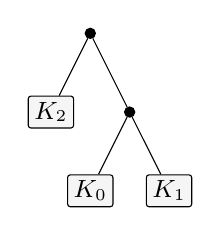
\begin{tikzpicture}[skeleton,level distance=10mm]
  \node[internal]{} child{node[atom]{$K_2$}} child{node[internal]{} child{node[atom]{$K_0$}} child{node[atom]{$K_1$}}};
\end{tikzpicture}
\hfill
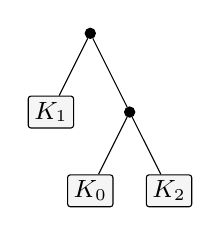
\begin{tikzpicture}[skeleton,level distance=10mm]
  \node[internal]{} child{node[atom]{$K_1$}} child{node[internal]{} child{node[atom]{$K_0$}} child{node[atom]{$K_2$}}};
\end{tikzpicture}
\hfill
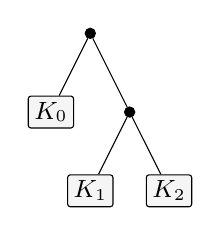
\begin{tikzpicture}[skeleton,level distance=10mm]
  \node[internal]{} child{node[atom]{$K_0$}} child{node[internal]{} child{node[atom]{$K_1$}} child{node[atom]{$K_2$}}};
\end{tikzpicture}\\[3mm]
leave $K_2$ at the root\qquad
leave $K_1$ at the root\qquad
leave $K_0$ at the root
\end{center}
\assembler{in words, writing $(A,B)$ for a node with children $A$ and $B$, the three pictured skeletons are
$(K_2,(K_0,K_1))$, $(K_1,(K_0,K_2))$ and $(K_0,(K_1,K_2))$.}
Each tree has two asymmetric binary nodes and class size $2^2=4$.  Thus $N_{\min}=3$.  The Fuss--Catalan value $C_6=132$ gives $132/2^2=33\equiv1\pmod2$, agreeing with $(-1)^2/(1!1!1!)\equiv1$.  Corollary~\ref{main:cor:exact-count} also gives $4!/(2!\,2^2)=3$.
\end{example}

\begin{example}[Ternary trees: $(p,k,n)=(3,1,8)$]\label{main:ex:ternary}
Now $m=17=9+2\cdot3+2\cdot1=122_3$, so $t=(5-1)/(3-1)=2$ and the atoms are $K_0,K_0',K_1,K_1',K_2$.  Corollary~\ref{main:cor:exact-count} gives
\[
 N_{\min}=\frac{6!}{2!\,3^2\,(2!\,2!\,1!)}=10.
\]
Two of the ten skeletons, using distinct labels for equal-height atoms, are
\begin{center}
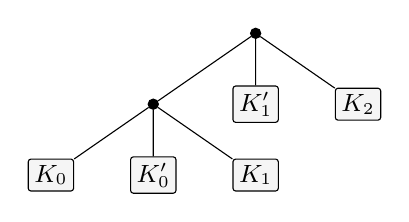
\begin{tikzpicture}[skeleton,sibling distance=13mm]
  \node[internal]{}
    child{node[internal]{} child{node[atom]{$K_0$}} child{node[atom]{$K_0'$}} child{node[atom]{$K_1$}}}
    child{node[atom]{$K_1'$}}
    child{node[atom]{$K_2$}};
\end{tikzpicture}
\qquad
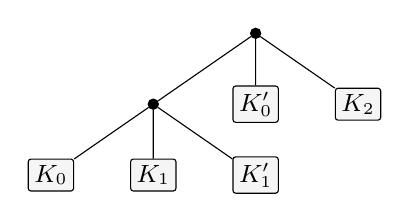
\begin{tikzpicture}[skeleton,sibling distance=13mm]
  \node[internal]{}
    child{node[internal]{} child{node[atom]{$K_0$}} child{node[atom]{$K_1$}} child{node[atom]{$K_1'$}}}
    child{node[atom]{$K_0'$}}
    child{node[atom]{$K_2$}};
\end{tikzpicture}
\end{center}
\assembler{in words, the two pictured skeletons are $((K_0,K_0',K_1),K_1',K_2)$ and
$((K_0,K_1,K_1'),K_0',K_2)$.}
Both pictured cherries contain a repeated height, so as unlabelled skeletons each cherry has a single cyclic order, and each pictured choice of atoms gives two skeletons, which differ by the cyclic order of the three children of the root.  Sorting the ten skeletons by the two atoms that sit at the root next to the internal node: $\{K_0,K_0\}$ and $\{K_1,K_1\}$ give one skeleton each; $\{K_0,K_2\}$ and $\{K_1,K_2\}$ give two each; $\{K_0,K_1\}$ gives four (two cyclic orders at the root times two for the cherry $K_0,K_1,K_2$).  In all $1+1+2+2+4=10$.  Since $k=1$, all atoms are in one depth class and the vector is $(5)$.  Distinct labelling yields $T(5)=10(2!2!)=40$.  Two applications of the carry congruence give
\[
 T(5)\equiv-T(5-3+1)=-T(3)\equiv T(1)\pmod3,
\]
so $T(5)\equiv1\pmod3$, as $40$ confirms.  Here $C_8^{(3)}=43263$, $43263/3^2=4807$, and $4807\equiv1\pmod3$.  Theorem~\ref{main:thm:main} predicts $(-1)^2/(2!2!1!)=4^{-1}\equiv1\pmod3$.
\end{example}

\begin{example}[Quaternary trees: $(p,k,n)=(2,2,4)$]\label{main:ex:quaternary}
In this case $q=4$ and $m=13=8+4+1=1101_2$, so $t=2$, with atoms $K_0,K_2,K_3$.  Condition (S) is now essential: at depth $r$,
\[
 K_0\text{ and }K_2\text{ require }r\equiv0\pmod2,
 \qquad K_3\text{ requires }r\equiv1\pmod2.
\]
A binary cyclic skeleton with two internal nodes has two leaves at depth $2$ and one leaf at depth $1$.  Therefore $K_3$ must be the leaf adjacent to the root, while $K_0$ and $K_2$ form the cherry at depth $2$:
\begin{center}
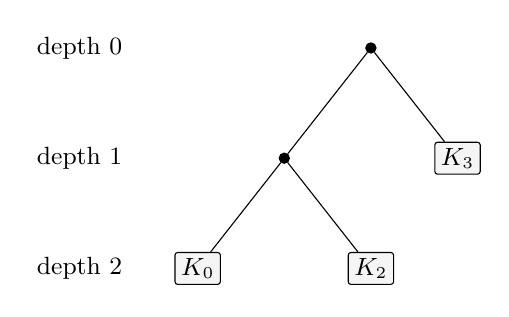
\begin{tikzpicture}[skeleton,level distance=14mm,sibling distance=22mm]
  \node[internal]{}
    child{node[internal]{} child{node[atom]{$K_0$}} child{node[atom]{$K_2$}}}
    child{node[atom]{$K_3$}};
  \node at (-3.7,0) {\small depth $0$};
  \node at (-3.7,-1.4) {\small depth $1$};
  \node at (-3.7,-2.8) {\small depth $2$};
\end{tikzpicture}
\end{center}
\assembler{in words, the pictured skeleton is $((K_0,K_2),K_3)$: the root at depth $0$; below it an
internal node and the atom $K_3$, both at depth $1$; below the internal node the atoms $K_0$ and $K_2$ at
depth $2$.}
After atom expansion, the leaves of $K_0$ are at depth $2$, those of $K_2$ at depth $2+2=4$, and those of $K_3$ at depth $1+3=4$.  All these depths are even, as required for $q=4$.  There is one minimal class.

For a labelled illustration of carrying, classes $0$ and $1$ in $\Z_2$ give the vector $\mathbf a=(2,1)$, since $K_0,K_2$ are labels of class $0$ and $K_3$ is of class $1$.  First carry the two class-$0$ labels, then the two resulting class-$1$ labels:
\[
 (2,1)\longrightarrow(0,2)\longrightarrow(1,0).
\]
Modulo $2$, the carry congruence reads $T(\mathbf a)\equiv-T(\mathbf a')\equiv T(\mathbf a')$.  Thus
\[
 T(2,1)\equiv-T(0,2)\equiv T(1,0)\pmod2.
\]
The actual values are all $1$, and $N_{\min}=1$.  Indeed $C_4^{(4)}=140$ and $140/2^2=35\equiv1\pmod2$.
\end{example}

% ---- Section 4 (in the numbering of the PDF): written by Claude Fable 5.2 (worker W046), 2026-11-15, from CLAIMS.md, FINDINGS.md and
% ---- notes/2026-11-14_carry_budget.md (the carry budget is transcribed from that note, written by Claude
% ---- Fable 5.2 as orchestrator). Not human-reviewed.
% ---- Revised 2026-11-15 by Claude Fable 5.2 (reviewer, brief W053): the first sentence of "Support" in
% ---- Section 4.2, and in Section 4.5 the parenthesis on the paper of Postnikov and Sagan (item on weights).
\section{Three further proofs, the carry budget, and extensions}\label{sec:further}
Three more proofs of the main theorem were produced during the event. Their full texts are
Appendices~\ref{app:path}, \ref{app:frob} and~\ref{app:acc}. This section says what each adds and how it is
supported; the precise status is in the table of Section~\ref{sec:status}.

\subsection{A proof on lattice paths (Appendix~\ref{app:path})}
\emph{What it is.} Take the words of length $N=n+m$ with $n$ letters \textsf{E} and $m$ letters \textsf{S}. Cut
the $N$ positions into $N_i$ consecutive segments of length $p^i$, where the $N_i$ are the base-$p$ digits of
$N$, and each segment into $p$ sub-segments, down to single letters; a move rotates the $p$ sub-pieces of one
segment. The class of a word has $p^d$ elements, $d$ being the number of segments whose $p$ sub-pieces are not
all equivalent (Lemma~\ref{path:lem:size}); $d\ge c$, the number of carries when $n$ and $m$ are added in base
$p$ (Proposition~\ref{path:prop:bound}); when $d=c$ there is exactly one mixed segment for each carry
(Lemma~\ref{path:lem:mixed}); so the classes with $d=c$ are counted by an explicit product, which Wilson's
theorem evaluates modulo $p$ (Proposition~\ref{path:prop:count}). This proves, for every binomial coefficient,
that $p^c$ divides $\binom Nn$ exactly, with the residue (Theorem~\ref{path:thm:binom}); the Fuss--Catalan
case follows from $\binom{qn+1}{n}=(qn+1)\,C_n^{(q)}$ (Theorem~\ref{path:thm:main}).

\emph{What it adds.} A second proof of the formula in which no factorial is valued and no cherry is
collapsed: on paths the skeleton is rigid, one mixed segment for each carry, so the smallest classes can be
counted level by level. It has the same plan as the main proof (class size $p^d$, a lower bound from digit
sums, minimal objects from the digits, a count modulo $p$). \emph{What it does not do:} the symmetry acts on
the $N\cdot C_n^{(q)}$ words, not on the $C_n^{(q)}$ trees, and the passage to $C_n^{(q)}$ uses one arithmetic
fact; so it is a companion to the main proof and not a proof ``from symmetries of the trees''.

\emph{Attribution and support.} The theorem is classical (Kummer; Anton, Stickelberger, Hensel
\cite{Granville}) and the mechanism is known \cite{Smith,Wildon}; see Section~\ref{sec:attribution} for what
exactly is in those sources and what was not found there. The written proof was read and verified by a
faculty member of the team. \PathLeanStatus

\subsection{A proof by algebra alone (Appendix~\ref{app:frob})}
\emph{What it is.} Start from $G=x+G^q$ only. For every power series $f$ with integer coefficients,
$f^p=f(x^p)+p\,\theta(f)$ with $\theta(f)$ again integral. Replace that factor $p$ by a variable $y$: for
$q=p$ this gives the equation $F=x+F(x^p,y^p)+y\,\theta(F)$, whose solution is $G$ at $y=p$
(Lemma~\ref{frob:lem:system}; for $q=p^k$ a system of $k$ such equations). Digit sums show that in the
coefficient of $x^m$ the lowest power of $y$ is $y^t$ (Lemma~\ref{frob:lem:lower}); its coefficient obeys the
same equation with a carry-free product (Lemma~\ref{frob:lem:lead}); and a derivative identity modulo $p$ in a
ring of Hurwitz series gives the carry rule (Proposition~\ref{frob:prop:carry}), hence the residue.

\emph{What it adds.} It shares no lemma with the main proof, so each is a check on the other, and it explains
the main proof: $y$ marks asymmetric nodes, so $y=p$ counts ordered trees, $y=1$ counts classes and $y=0$
keeps only the complete trees, $x+x^p+x^{p^2}+\cdots$ (the dictionary is in Section~\ref{frob:sec:dict}; it
is not used in the proof, and that the coefficient of $x^my^d$ is the number of classes with $m$ leaves and
$d$ asymmetric nodes was confirmed by computation only). For $p=2$: the coefficient of $x^5$ is $y+y^2+y^3$
and that of $x^6$ is $y+2y^2+2y^3+y^4$, which at $y=2$ give $14$ and $42$; these two polynomials are already
in Etherington's paper \cite{Etherington}, whose equation~(33) is the case $p=2$, $k=1$ of the deformed
equation. It is algebra, not ``symmetries of trees'', so it is not offered as the answer to the problem.

\emph{Support.} A team member began to read this proof and stopped for the time being; no human has checked
it. One AI referee and computer checks of every lemma found no error. It is formalized in Lean in full (Section~\ref{sec:lean}); a dependency listing produced by Lean shows
that the formal proof reaches no rotation, no class of trees and no cherry of the first formal proof.

\subsection{An accounting proof: every node is worth $-p$ (Appendix~\ref{app:acc})}
\emph{What it is.} Label all $m$ leaves. A $p$-ary tree with $m$ leaves has $N(m)=(m-1)/(p-1)$ internal nodes
(this $N(m)$ is not the $N=n+m$ of the lattice-path proof);
with distinct labels each is asymmetric and contributes a factor $p$, and the carry proposition of the main
proof contributes a sign $-1$ for each: $m!\,C_n^{(q)}=p^{N(m)}L(m)$ with $L(m)\equiv(-1)^{N(m)}\pmod p$
(Lemma~\ref{acc:L1}). On the other side, $m!=p^{\nu}\prod_jm_j!\,|\F(m)|$ with $\nu=\nu(m)=(m-s_p(m))/(p-1)$ and
$|\F(m)|\equiv(-1)^{\nu}\pmod p$, where $\F(m)$ is a set of ``digit-forest structures''
(Lemmas~\ref{acc:L3} and~\ref{acc:L4}; together they are Legendre's formula with its residue, proved by the
same kind of symmetry argument). Dividing gives $C_n^{(q)}\prod_jm_j!\equiv(-p)^{t}\pmod{p^{t+1}}$ with
$t=N(m)-\nu$.

\emph{What it adds.} The one-line form of the theorem, and a reading of $t$ as a difference: with the rule
``$p$ grains on a site topple into one grain on the next site'', $v_p(C_n^{(q)})$ is the number of topplings of
$m$ grains on a ring of $k$ sites minus the number on a half-line (the proposition at the end of
Appendix~\ref{app:acc}). With $\varpi$ a root of $z^{p-1}+p=0$, so that $\varpi^{p-1}=-p$ (the constant of
Dwork's exponential, see \cite{Kochubei}; it is not the number $\pi=\zeta_p-1$ of
Section~\ref{sec:connections}), Lemma~\ref{acc:L1} reads $C_n^{(q)}=(\varpi^{m-1}/m!)\cdot u$ with $u$ an
integer $\equiv1\pmod p$. \emph{What it does not do:} it depends on the carry proposition of the main proof,
and it computes $v_p(m!)$ (by symmetry, not by quoting Legendre); whether that meets ``without factorial
valuations'' is left to the reader.

\emph{Support.} Read by a faculty member of the team (``looks like it makes sense''; not signed); one AI
referee; computer checks of the lemmas. Lean checks the two conclusions by a classical route, not this
argument.

\subsection{The carry budget: a second proof of the lower bound}\label{sec:carrybudget}
This subsection is transcribed from a note of the project (claim C19), with one marked note on notation
added on 15 November. It proves again
Proposition~\ref{main:prop:lower-bound} and the criterion of Proposition~\ref{main:prop:minimal-local}, from
one identity and without induction on the tree. \emph{Status:} checked only by AI (one AI referee found the
mathematics correct; one wrong sentence in an analogy and some gaps of statement were repaired and not
re-reviewed), by computation, and since 15 November by Lean (Facts~1 to~3 and the criterion for
$d=t$; Section~\ref{sec:lean}); no human has read it.

Let $T$ be a $p$-ary tree with $m$ leaves. For a vertex $v$ let $m_v$ be the number of leaves below it
($m_v=1$ for a leaf), and let $N=(m-1)/(p-1)$ be the number of internal nodes.
% Clarification added 2026-11-15 after the referee report (report/reviews/REFEREE.md, finding 10); not in the text that was reviewed.
\refnote{this $N$ is the $N(m)$ of the accounting proof (Appendix~\ref{app:acc}); it is not the $N=n+m$ of the
lattice-path proof.}
A \emph{carry} is one trade of
$p$ units in a column for one unit in the next column; it lowers the sum of the digits by $p-1$. (When $p$
numbers are added, one column may need several trades, and each counts: in base $3$, $12_3+12_3+12_3=120_3$
makes three carries.) For a node $v$ with children $v_1,\dots,v_p$ put
\[
 c(v)=\frac{s_p(m_{v_1})+\dots+s_p(m_{v_p})-s_p(m_v)}{p-1}\ \ge0 ,
\]
the number of carries made when the leaf counts of the children are added in base $p$ (an integer $\ge0$ by
Lemma~\ref{main:lem:digit}).

\medskip\noindent\textbf{Fact 1 (the budget is fixed).} \emph{For every tree with $m$ leaves,
$\sum_vc(v)=(m-s_p(m))/(p-1)=:\nu(m)$, the sum being over the internal nodes.}

\emph{Proof.} In $\sum_v\bigl[\sum_is_p(m_{v_i})-s_p(m_v)\bigr]$ every vertex other than the root appears once
with a plus sign (as a child), and every internal node appears once with a minus sign (as a parent). So
everything cancels except the leaves, each contributing $s_p(1)=1$, and the root, contributing $-s_p(m)$.
(For $m=1$ there is no node and both sides are $0$.) \qed

\medskip\noindent\textbf{Fact 2 (a symmetric node always carries).} \emph{If $v$ is symmetric, its children
all have the same number $b$ of leaves, and $c(v)=(p\,s_p(b)-s_p(pb))/(p-1)=s_p(b)\ge1$.} (Equivalent trees
have the same number of leaves, Lemma~\ref{main:lem:depth-invariant}, and $s_p(pb)=s_p(b)$.) Consequently a
node that makes no carry is asymmetric.

\medskip\noindent\textbf{Fact 3 (the excess formula).} \emph{Let $\sigma$ be the number of symmetric nodes, so
$d(T)=N-\sigma$. Since $t=N-\nu(m)$,}
\[
 d(T)-t=\nu(m)-\sigma=\sum_{v\ \mathrm{symmetric}}\bigl(s_p(b_v)-1\bigr)+\sum_{v\ \mathrm{asymmetric}}c(v),
\]
\emph{where $b_v$ is the number of leaves of a child of the symmetric node $v$. Every term on the right is
$\ge0$.} (This is Fact~1 with the sum split by the type of node, and Fact~2.)

\medskip\noindent\textbf{Consequences.} (1) $d(T)\ge t$: there are only $\nu(m)$ carries to go round, every
symmetric node uses at least one, so at most $\nu(m)$ nodes are symmetric and at least $N-\nu(m)=t$ are
asymmetric. For example a binary tree with $13=1101_2$ leaves has $12$ nodes and makes $10$ carries, so at
most $10$ nodes are symmetric and at least $2$ are asymmetric. (2) $d(T)=t$ if and only if (a) every
asymmetric node adds the leaf counts of its children without a carry, and (b) every symmetric node has
children whose number of leaves is a power of $p$. The note derives from (a) and (b) the description of the
minimal trees by the digits of $m$, which is Proposition~\ref{main:prop:skeleton} for $k=1$; that derivation
is not reproduced, since the proposition is proved in Section~\ref{sec:mainproof}.

\medskip\noindent\textbf{Remarks} (from the same note; not used anywhere). Facts~1 to~3 and the two
consequences use nowhere that $p$ is prime; they hold for trees of any arity $r\ge2$ with base-$r$ digits.
The rotations that map a tree to itself form a group of order $p^{\sigma}$ which permutes the $m$ leaves
faithfully; so $\sigma\le v_p(m!)$, with equality exactly when this group is a Sylow $p$-subgroup of the
symmetric group on the leaves. By Legendre's formula $v_p(m!)=\nu(m)$, and $\sigma=\nu(m)$ exactly when $d=t$
by Fact~3. So \emph{the minimal trees are exactly the trees whose symmetry group is a Sylow $p$-subgroup of
the symmetric group on their leaves.} This remark is the one place in this subsection where a factorial
appears. (Checked by computation on explicit groups for small trees, claim C23(c); the proof of the group
order is sketched in the note and is not reproduced here.)

\subsection{Extensions: other statistics}\label{sec:extensions}
The problem statement suggests weighted numbers and other statistics. The first three items below are proved:
the proofs are a few lines from Steps~1 and~2, and all three statements are checked by Lean
(Section~\ref{sec:lean}). They were written on the last night of the event, and no human has read them. An AI
referee read them on 15 November and wrote out one step that the two corollaries had used without proof
(rotations do not change the depths of the internal nodes); the present wording of the proofs is the
referee's and has had no other reader. Of the
remaining items, C9 and C17 are conjectures supported by the computations listed in
Section~\ref{sec:computations}, and C27 is checked by Lean but has no written proof in this report.
\begin{itemize}[itemsep=1pt]
\item \emph{Closed families} (C11). A set $F$ of $p$-ary trees is \emph{closed under rotation} if $T\in F$
 and $T'\sim T$ imply $T'\in F$, where $\sim$ is the rotation equivalence of Section~\ref{sec:mainproof}.
 \textbf{Proposition.} \emph{Let $m\equiv1\pmod{p-1}$ and $t=(s_p(m)-1)/(p-1)$, and let $F$ be a set of
 $p$-ary trees with $m$ leaves that is closed under rotation ($F$ may be empty). Then $p^t$ divides $|F|$, and
 $|F|\equiv p^t\cdot\#\{\text{rotation classes in }F\text{ with }d=t\}\pmod{p^{t+1}}$.}
 \emph{Proof.} $F$ is a union of rotation classes. A class has $p^{d}$ members
 (Lemma~\ref{main:lem:class-size}) and $d\ge t$ (Proposition~\ref{main:prop:lower-bound}). The classes with
 $d>t$ contribute multiples of $p^{t+1}$, and each class with $d=t$ contributes $p^t$. \qed

 So every statistic of $p$-ary trees that rotations do not change refines the divisibility of the theorem: the
 number of trees with $m$ leaves and a prescribed value of the statistic is divisible by $p^t$.

 For $q=p^k$ with $k\ge2$ this is a statement about the blocked form (Lemma~\ref{main:lem:blocked}): a set of
 $q$-ary trees is called closed under rotation if the set of the corresponding $k$-blocked $p$-ary trees is
 closed under rotation; rotations map $k$-blocked trees to $k$-blocked trees
 (Lemma~\ref{main:lem:depth-invariant}). In terms of the $q$-ary tree, the $q$ children of a node are then
 permuted by the group that the rotations at the $k$ levels of its block generate: the group of the remark
 after the definition of $\sim$ in Section~\ref{sec:mainproof}, of order $p^{(q-1)/(p-1)}$ (one rotation for
 each of the $(q-1)/(p-1)$ nodes of the block). For $k\ge2$ this is not the group of cyclic shifts of the $q$
 children: for $q=4$ it is generated by the permutations $(1\,2)$, $(3\,4)$ and $(1\,3)(2\,4)$ of the four
 children, has $8$ elements, and does not contain the shift $(1\,2\,3\,4)$ (compare the items on mobiles and
 on quadtrees in Section~\ref{sec:connections}). A statistic that is invariant only under cyclic shifts of the
 $q$ children is not covered by the proposition.
\item \emph{Level profiles} (C10). \textbf{Corollary.} \emph{Let $q=p^k$, let $n_0=1,n_1,\dots,n_{L-1}$ be
 non-negative integers, $n_L=0$, $n=\sum_{i<L}n_i$ and $t=(s_p((q-1)n+1)-1)/(p-1)$. Then}
 \[
  p^t\ \Big|\ \prod_{i<L}\binom{q\,n_i}{n_{i+1}} .
 \]
 \emph{Proof.} The product is the number of $q$-ary trees that have exactly $n_i$ internal nodes at depth $i$
 for every $i\le L$ (and therefore none at any depth $\ge L$): the $n_i$ nodes at depth $i$ have $q\,n_i$
 children, and $n_{i+1}$ of these are chosen to be internal nodes; if some $n_i=0<n_{i+1}$ there is no such
 tree and the product is $0$. In the blocked form (Lemma~\ref{main:lem:blocked}) the internal nodes of the
 $q$-ary tree at depth $i$ become the roots of the blocks at depth $ik$, and these are all the internal nodes
 of the $p$-ary tree at depth $ik$. So the trees in question become the set $F$ of the $k$-blocked $p$-ary
 trees with $(q-1)n+1$ leaves that have exactly $n_i$ internal nodes at depth $ik$ for every $i\le L$.
 Rotation-equivalent trees have the same multiset of depths of internal nodes. The proof is that of
 Lemma~\ref{main:lem:depth-invariant}: ``the same multiset of depths of internal nodes'' is an equivalence
 relation on $p$-ary trees, and it satisfies (R1) and (R2), because the depths of the internal nodes of
 $(U_1,\dots,U_p)$ are $0$, for the root, and those of the $U_i$, each increased by $1$; so it contains
 $\sim$. Together with Lemma~\ref{main:lem:depth-invariant} this shows that $F$ is closed under rotation, and
 the proposition applies with $m=(q-1)n+1$. \qed

 The sum of these products over all profiles with $\sum_in_i=n$ is $C_n^{(q)}$, so the corollary refines the
 divisibility half of the theorem; it is a statement about binomial coefficients, and its proof uses no
 valuation of a factorial. For the formal proof this is supported by a listing that the Lean build prints
 (file \file{lean/MMM/AxiomsExtra.lean}): the declarations in the full closure of the theorem, through Mathlib
 and the core library, whose names contain one of nine strings such as \texttt{multiplicity\_choose},
 \texttt{multiplicity\_factorial}, \texttt{padicval}, \texttt{legendre}, \texttt{kummer} or \texttt{lucas}
 (Section~\ref{sec:lean}). The list is empty. The statement was computed beforehand for every profile
 in the ranges of Section~\ref{sec:computations}. It was not found in the four papers that an AI system read in full early
 in the project to look for overlap; no other search of the literature was made for it, and we do not claim
 that it is new.
\item \emph{Weights that rotations do not change} (C28). \textbf{Corollary.} \emph{Let $w$ be an
 integer-valued function on $p$-ary trees with $w(S)=w(T)$ whenever $S\sim T$, let $m\equiv1\pmod{p-1}$ and
 $t=(s_p(m)-1)/(p-1)$, and let $F$ be a set of $p$-ary trees with $m$ leaves that is closed under rotation.
 Then $p^t$ divides $\sum_{T\in F}w(T)$. In particular, for $q=p^k$ and arbitrary integers $b_0,b_1,\dots$,}
 \[
  p^t\ \Big|\ \sum_{T}\ \prod_{v}b_{\operatorname{depth}(v)},\qquad t=\frac{s_p((q-1)n+1)-1}{p-1},
 \]
 \emph{the sum over the $q$-ary trees $T$ with $n$ internal nodes, the product over the internal nodes $v$
 of $T$, and $\operatorname{depth}(v)$ the depth of $v$ in the $q$-ary tree.}
 \emph{Proof.} $F$ is a union of rotation classes; the sum of $w$ over a class of $p^d$ trees is $p^d$ times
 the value of $w$ on the class, and $d\ge t$ (Lemma~\ref{main:lem:class-size},
 Proposition~\ref{main:prop:lower-bound}). For the second statement put
 $w(U)=\prod_ib_i^{\,n_i(U)}$ for a $p$-ary tree $U$, where $n_i(U)$ is the number of internal nodes of $U$ at
 depth $ik$. Rotations do not change the numbers $n_i(U)$ (proof of the previous corollary), so $w$ takes the
 same value on rotation-equivalent trees. Let $F$ be the set of all $k$-blocked $p$-ary trees with
 $m=(q-1)n+1$ leaves; it is closed under rotation (Lemma~\ref{main:lem:depth-invariant}) and corresponds to the
 $q$-ary trees with $n$ internal nodes (Lemma~\ref{main:lem:blocked}), and for a blocked tree $U$ the number
 $w(U)$ is the weight $\prod_vb_{\operatorname{depth}(v)}$ of the corresponding $q$-ary tree, whose internal
 nodes at depth $i$ are the internal nodes of $U$ at depth $ik$. \qed

 With all $b_i=1$ this is the divisibility half of the theorem. It is \emph{not} the weighted theorem of
 \cite[Theorem~5]{Konvalinka}, which is quoted in the next item:
 there the weight of a vertex depends on the number of non-right edges on the path from the root, which
 rotations change, and the conclusion is a congruence, not only a divisibility. (Of the paper
 \cite{PostnikovSagan} on weighted Catalan numbers the project has one reading: an AI system read the full
 text of its arXiv version on the first day of the event, to look for overlap with the main proof; no person
 has read it, and the corollary is not compared with that paper here.) The corollary says nothing
 about exactness; it records what the rotation argument gives for weights with no further idea. Tested
 beforehand on random integer weights ($q\in\{2,3,4,5,8,9\}$, $n\le14$; the program is not kept in the
 repository). No search of the literature was made for it.
\item \emph{Weighted Fuss--Catalan numbers} (C9), a conjecture. What follows about \cite{Konvalinka} is taken
 from the project's reading notes and says no more than they do. A vertex $v$ of a $q$-ary tree gets the
 weight $b(i_v)$, where $i_v$ is the number of non-right edges on the path from the root to $v$, and the
 weighted number is $C_n^{(q)}(b)=\sum_T\prod_vb(i_v)$ (the notes give this formula without saying more; we
 read $T$ as running over the $q$-ary trees with $n$ internal nodes). Theorem~5 of that paper: \emph{if $b(0)\equiv1\pmod q$ and $q^{j+1}$ divides $\Delta^jb(x)$ for all
 $j\ge1$ and all $x$, then $C_n^{(q)}(b)\equiv C_n^{(q)}\pmod{p^{t+k}}$.} (The notes do not define $\Delta$;
 the program of the experiment named below checks this hypothesis by finite differences.) This is a theorem of
 \cite{Konvalinka}, and its statement mentions no group. \emph{The conjecture C9}, in the words of the
 project's ledger, is about its proof: Konvalinka's proof of Theorem~5 works unchanged with the rotation group
 of this report in place of the full symmetric group, because the proof only needs the group to be transitive
 on the $q$ branches of a node, and the rotation group is transitive. If that is so, the weighted theorem
 also becomes free of factorial valuations. It has not been written out as a proof. \emph{What was computed}
 (experiment E002, with the orbits of the rotation group): for $q\in\{2,3,4,5,8,9\}$ and four weight functions
 for each $q$, no failure of the four checks that the ledger records (integrality, residue, recurrence, and
 the congruence modulo $p^{t+k}$); with a control group that is not transitive on the branches, the
 recurrence fails in $4122$ of $4224$ comparisons. The weight $b(i_v)$ is changed by rotations, so C9 is not a
 case of the corollary above. Supported numerically; not proved.
\item \emph{A bijection} (C17): cyclic $p$-ary trees with $(p-1)t+1$ labelled leaves and permutations of $pt$
 points with $t$ cycles of length $p$; it would give Corollary~\ref{main:cor:exact-count} without the
 Fuss--Catalan formula. Checked in small cases only.
\item \emph{A product formula for minimal words over arbitrary lists of blocks} (C27), a generalisation of
 Proposition~\ref{path:prop:count} that was formulated as the statement for an induction in Lean. It is
 checked by Lean and by computation; there is no written proof in this report.
\end{itemize}
Not explored: $q$ that is not a prime power; residues modulo $p^2$.


% ---- Section 5 (in the numbering of the PDF): written by Claude Fable 5.2 (worker W046), 2026-11-15, from
% ---- notes/2026-11-14_connections_ranked.md, notes/2026-11-14_motivation_and_connections.md, CLAIMS.md
% ---- (C15, C21, C22, C23, C25, C26) and the two slide decks. Not human-reviewed.
% ---- Revised 2026-11-15 by Claude Fable 5.2 (reviewer, brief W053): in item 1 the sentence on the four
% ---- pictures of one tree (reworded, content unchanged); in item 5 the reading status of the cited survey.
\section{Connections with other fields}\label{sec:connections}
The trees of the theorem occur in several sciences, and in none of them does the left-to-right order of the
branches mean anything: what matters is the shape, and the question ``how many ordered trees stand over one
shape?'' has the answer $p^d$ of Step~1. This section lists the connections that the team's slides show, each
with its status: \textbf{[known]} means a statement of the other field, taken from a source in the reference
list (all of these sources were opened by AI systems only; none was read by a human on the team, and no
practitioner of these fields was consulted); \textbf{[computed]} means an observation of the project, checked
by computer in the stated range and not proved here unless it is a restatement of a result of
Section~\ref{sec:mainproof}; \textbf{[analogy]} means a way of speaking with no claim attached. None of this
is used in any proof. The project ranked 43 candidate connections by how much of the method each contains;
the first five are items 1 to 5.

\begin{enumerate}[leftmargin=1.6em,itemsep=3pt]
\item \textbf{Evolutionary trees ($p=2$): prior work.} \textbf{[known]} A rooted binary tree shape with $m$
leaves and $\sigma$ ``symmetry nodes'' (nodes whose two subtrees have the same shape; the symmetric nodes of
Section~\ref{sec:carrybudget}) has $m!/2^{\sigma}$ labellings by
$m$ species \cite{Steel2014,BonaFlajolet}; the number of nodes that are not symmetry nodes is a balance index
of the tree, its minimum over trees with $m$ leaves is $s_2(m)-1$, attained by the trees built from the binary
digits of $m$, of which there are $(2s_2(m)-3)!!$ \cite{KerstingFischer}. This is Steps~2 and~3 and the odd
count for $p=2$, found without reference to Catalan numbers; two leaves with a common parent are called a
cherry in that field. \textbf{[computed; the formula is in the literature]} In the Yule model, defined by
uniform splitting, the probability of a shape is $2^{d}/\prod_v(m_v-1)$, $m_v$ the number of leaves below the
node $v$, with our $d$ (\cite{Steel2025} states the Yule--Harding probability as $2^{n-1-s}/\prod n(v)$, in
its notation). \textbf{[computed]} Exchanging two labels fixes a labelled tree exactly when the two leaves form a cherry
($m\le7$). One tree with $6$ leaves can be drawn as an evolutionary tree, a knockout tournament, a prefix
code and a bar of music (four pictures of one slide of the talk); $6=110_2$, so one node has to be lopsided,
and one is enough.

\item \textbf{Sylow subgroups of symmetric groups (every $p$ and $q$).} \textbf{[known]} The group that the
proof puts at a $q$-ary node, rotations at $k$ levels of $p$-ary nodes, is an iterated wreath product of
cyclic groups of order $p$ and a Sylow $p$-subgroup of the symmetric group $S_q$ (\cite{GiannelliLaw} for odd
$p$; for $p=2$, as the automorphism group of the complete binary tree, \cite{DeutschSagan}); a Sylow
$p$-subgroup of $S_m$ is a product over the base-$p$ digits of $m$ \cite{Kaloujnine}, and the construction
by nested blocks with rotations is in \cite{Smith}. \textbf{[computed; proof sketched in the project's note, not
reproduced]} A tree is minimal ($d=t$) exactly when the group of rotations that fix it is a Sylow
$p$-subgroup of the permutations of its leaves (Section~\ref{sec:carrybudget}; explicit groups for trees with at most $9$ nodes
when $p=2$, at most $6$ nodes when $p=3$, at most $4$ nodes when $p=5$). In this language the bound of Step~2 would follow from Legendre's
formula in one line; that is the proof the problem excludes, and Step~2 derives the bound from carries
instead.

\item \textbf{Alkyl groups (chemistry, $p=3$).} \textbf{[known]} The three further bonds of a carbon atom can
be rotated, not reflected: the group at a carbon is cyclic of order $3$ \cite{RHB}. Ternary trees up to
rotation are the alkyl groups C$_n$H$_{2n+1}$ with mirror images counted separately:
$1,1,2,5,11,28,74,\dots$ \cite{OEISA000625}; their generating function satisfies
$A(x)=1+x(A(x)^3+2A(x^3))/3$, an equation that the OEIS entry refers to P\'olya \cite{Polya} (his
equation~(25)). \textbf{[computed]} The deformed equation of Appendix~\ref{app:frob} for $p=3$, $k=1$,
indexed by the number of nodes, becomes this equation at $y=1$ ($n\le14$). \textbf{[computed]} For four
carbons there are five (\emph{tert}-butyl,
isobutyl, the two mirror forms of \emph{sec}-butyl, $n$-butyl), and over them stand $1,9,9,9,27$ ordered
ternary trees: $55=1+9+9+9+27$ is not divisible by $3$ because \emph{tert}-butyl is alone in its class. The
ternary tree numbers are prime to $3$ exactly for $n=1,4,13,40,\dots$, the sizes at which a perfectly branched
group exists (this case $t=0$, with residue $1$, is in the OEIS without proof \cite{OEISA201823}).
\textbf{[computed; the reading is ours]} For a rooted ternary tree with $n$ nodes, (class size) $\times$
$3^{\text{number of symmetric nodes}}=3^n$; for the five butyl groups the pairs are $(1,81)$, $(9,9)$, $(9,9)$,
$(9,9)$, $(27,3)$. The second factor is the internal symmetry number of the group by the rule that
thermochemists use \cite{DomalskiHearing}, for a group attached to a partner without symmetry of its own; the
values tabulated in that reference are for whole molecules and are \emph{not} values of the model (an earlier
wording of the project that said otherwise was withdrawn). The ordered ternary trees with $n$ nodes, taken up
to rotation at the root only, are counted by the sequence \cite{OEISA121179} ($n\le8$), which a comment in that
entry describes as the number of staggered conformers of alkyls. With chemists in the room, a node of ours whose three
branches are not all alike should be called ``lopsided'', not ``asymmetric carbon'', which means something
narrower. \textbf{[computed]} A second agent session run by a team member compared the model with printed
tables up to $14$ carbons (stereoisomers, structural isomers, achiral ones) and found agreement; under all
permutations the five classes for $n=4$ become four, of sizes $1,9,18,27$.

\item \textbf{Mobiles (every prime $p$).} \textbf{[analogy, with a known name]} Hang a tree from the ceiling:
every bar can spin, a drawing of the tree is a photograph of the mobile, and a mobile with $d$ lopsided bars
has $p^d$ photographs (Step~1). So the number of drawings is a sum of powers of $p$, one for each mobile, and
its power of $p$ is the smallest that occurs, provided the number of mobiles with that power is not divisible
by $p$: the plan of the proof. Trees up to rotation at each node are called mobiles in the OEIS
\cite{OEISmobiles}. For a prime power the picture fails: a hub with four arms turns in $4$ ways, while the
proof's group at a $4$-ary node has $8$ elements.

\item \textbf{Quadtrees ($q=4$).} \textbf{[known]} Cutting a square into four quarters, and some of the
quarters again, is how quadtrees store images (\cite{Samet}, cited from its bibliographic record only; its
text was not opened); the pictures with $n$ cuts are the $4$-ary trees
with $n$ nodes. \textbf{[computed]} The eight symmetries of a square permute its four quarters and keep the
two diagonals together; as permutations of the quarters they are exactly the group the proof puts at a
$4$-ary node (two levels of binary nodes), of order $8$ among the $24$ permutations. Turning or mirroring any
cut square in place sorts the pictures into families of $2^d$ members; with three cuts, $22=2+4+16$, and the
number of families agrees with \cite{OEISmobiles} (A398109) for $n\le5$. For comparison, with all $24$
permutations at a node the classes have sizes such as $6$ and $12$; with the $8$ rotations they have sizes
$1,2,4,8$ (``bits, not bytes'': rotate at each of the $k$ levels of $p$-ary nodes instead of permuting the
$q$ branches). The picture is special to $q=4$: a cube has too few symmetries for $q=8$.

\item \textbf{The answer in one picture.} \textbf{[restatement of Step~3]} The most symmetric tree with $13$
leaves is made of complete trees with $8$, $4$ and $1$ leaves, because $13=1101_2$: the digits are the
building blocks. \textbf{[computed]} The Merkle tree that the Certificate Transparency standard prescribes
for $n$ entries \cite{RFC6962} is such a minimal tree. Letting $13$ single leaves fuse in equal pairs until
nothing can fuse leaves $8+4+1$ after $10$ fusions; each fusion is a carry (Section~\ref{sec:carrybudget}).
\textbf{[known]} Merging two binomial queues with $n$ and $n'$ items takes exactly
$s_2(n)+s_2(n')-s_2(n+n')$ comparisons \cite{Vuillemin}; that this is the number of carries of $n+n'$, and the
link to the theorem, are our remarks.

\item \textbf{Energy levels.} \textbf{[analogy over exact arithmetic]} Sort the $132$ binary trees with $7$
leaves by $d$: $132=3\cdot4+3\cdot8+4\cdot16+1\cdot32$. For a $2$-adic observer $2^d$ is small when $d$ is
large, so the lowest row decides: the valuation is the ``ground-state energy'' and the residue counts the
ground states modulo $p$. \textbf{[computed; the formula is known]} For $p=2$ the classes with $m$ leaves are
the tree diagrams, with $m$ sources and one marked point, of a field theory with a cubic interaction (setting
of \cite{Argyres}); a diagram is divided by its symmetry factor, which is $2^{\text{number of symmetric
vertices}}$ (the order of the automorphism group of a binary tree shape, \cite{BonaFlajolet}), and
$\tfrac3{16}+\tfrac38+\tfrac44+\tfrac12=\tfrac{33}{16}=C_6/2^6$. That $16$ appears as ``the denominator''
depends on writing the coupling as $g/3!$; this item was taken out of the project's first five for that
reason.

\item \textbf{Cuts into balls.} \textbf{[exact, elementary]} A binary tree with $m$ leaves is the same thing
as a complete prefix code with $m$ words, a cut of an interval into $m$ pieces by repeated halving, and a cut
of the $2$-adic integers into $m$ balls; so $C_{m-1}$ counts the cuts of the $2$-adic integers into $m$ balls,
and for $p$-ary trees $2$ is replaced by $p$. \textbf{[analogy]} In a computer the same cuts are blocks of
addresses; for $q=2^8$ the blocks are aligned to whole bytes.

\item \textbf{Polymers and triangles ($p=3$).} \textbf{[computed from a formula in the literature]}
Stockmayer's combinatorial factor for $n$ units with $f$ reactive groups, as given in \cite{Tanaka}, equals
the Fuss--Catalan number for $q=f-1$ divided by the number $(f-2)n+2$ of free groups. \textbf{[analogy]} A
tree-like molecule with $m$ ends can be perfectly branched only if $m$ is a power of $p$; otherwise it is $t$
junctions short. \textbf{[computed; the bijection is known]} Stacked triangulations (put a point inside a
triangle, join it to the corners, repeat) correspond to ternary trees \cite{AlbenqueMarckert}; turning the
inside of a cut triangle by a third of a turn is the rotation of the proof, and with three inner points
$12=3+9$.

\item \textbf{Light ($p=2$).} \textbf{[computed, with a caveat]} A nonlinear crystal fuses two photons into
one. In the history of a photon of the $m$-th harmonic, read as a binary tree with $m$ leaves, at least
$s_2(m)-1$ fusions are mixings of two different photons (all shapes up to $m=20$; it is Step~2). A real
apparatus can reuse a beam; then the count can drop, first at $m=15$.

\item \textbf{Sand.} \textbf{[proved in Appendix~\ref{app:acc}]} With the rule ``$p$ grains on a site topple
into one grain on the next site'', $v_p(C_n^{(q)})$ is the number of topplings of $m$ grains on a ring of $k$
sites minus the number on a line.

\item \textbf{Gauss sums.} \textbf{[computed; open question]} With $\pi=\zeta_p-1$, the residue formula has
the shape of Stickelberger's congruence for Gauss sums as quoted in \cite{Blache}; a computer test confirms,
in $77$ cases, that to leading order $C_n^{(q)}$ is $-1/\pi$ times the Gauss sum of exponent $m$. Whether this
is a known remark has not been established; no human has looked at it.
\end{enumerate}

\noindent Identifications of sequences: the numbers of rotation classes of binary, ternary, $5$-ary and
$7$-ary trees and of $4$-ary trees with $n$ nodes were found in the OEIS (A001190, A000625, A036727, A036728,
A398109) by looking up computed values (claim C15); these are lookups, not proofs.


% ---- Section 6 (in the numbering of the PDF): written by Claude Fable 5.2 (worker W046), 2026-11-15, from CLAIMS.md (ranges as recorded
% ---- there) and AI_USAGE.md. The assembler did not rerun the experiments. Not human-reviewed.
\section{Computations}\label{sec:computations}
A computation supports a statement in the range computed; it says nothing about a proof. The table lists
what was computed, over what range, by which program, and with what result. The folders
\file{experiments/E000_...} to \file{experiments/E017_...} of the repository contain the code, the output and a
description of each experiment (two folders begin with \file{E017}; the one meant below is
\file{E017_path_slot_count}); the two guest sessions keep theirs in their own folders. The ranges below are
those recorded in the project's ledger; the experiments were not rerun for this report, except for the five
values in the table of Section~\ref{sec:smallexamples} and for the recomputations of the AI referee in the
last row of the table. All programs were written by AI systems
(Section~\ref{sec:ai}); in the last column, ``independent'' means a second program that shares no code with
the first.

{\small
\setlength{\tabcolsep}{4pt}
\begin{longtable}{@{}>{\raggedright\arraybackslash}p{0.12\textwidth}>{\raggedright\arraybackslash}p{0.29\textwidth}>{\raggedright\arraybackslash}p{0.33\textwidth}>{\raggedright\arraybackslash}p{0.19\textwidth}@{}}
\toprule
Experiment & What was checked & Range & Result\\
\midrule
\endfirsthead
\toprule
Experiment & What was checked & Range & Result\\
\midrule
\endhead
\bottomrule
\endfoot
E000 & C1 to C8 by brute force: class sizes, the bound, minimal classes against skeletons, the carry
 congruence, the residue & small trees; $47$ cases for the class sizes, $307$ cases for the carry congruence
 & all pass\\\addlinespace[3pt]
E001 & the same, by code of a different model & $k=1$ and small $n$ only; $k>1$ and most labelled cases were
 not completed & agrees (independent)\\\addlinespace[3pt]
E003 & C1, C2, C6, C7, C8, with the full polynomials $\sum_{\text{classes}}y^d$ and nothing assumed &
 $1067$ values of $m$, up to about $400$ leaves; $p\in\{2,3,5,7,11,13\}$ for $k=1$;
 and $(p,k)=(2,2)$, $(3,2)$, $(5,2)$, $(2,3)$, $(3,3)$, $(2,4)$ & no failure\\\addlinespace[3pt]
(inline) & the compact form C12 & $885$ cases, $p\le11$, $k\le3$, $n<60$ & no failure\\\addlinespace[3pt]
E002 & C9 (weighted numbers), C10 (level profiles), C11 (two closed families) & C9: $q\in\{2,3,4,5,8,9\}$, four
 weight functions each; C10: every profile with $n\le22$ ($q=2$), $\le15$ ($q=3$), $\le14$ ($q=4,5$), $\le12$
 ($q=8,9$); C11: bounded height and ``all leaves deep'', $p=2$ ($n\le16$), $p=3$ ($n\le13$) & no failure; a
 control with a non-transitive group fails, as predicted\\\addlinespace[3pt]
E007 & C11 for five rotation-invariant statistics & $q\in\{2,3,4,5,8,9\}$, small $n$ & no failure\\\addlinespace[3pt]
E004 & the lemmas of the accounting proof, with the digit forests listed explicitly & $24$ cases including
 $k=2,3$ (the two statements of Lemma~\ref{acc:L1}); $27$ cases (Lemmas~\ref{acc:L3}, \ref{acc:L4}) & all pass\\\addlinespace[3pt]
(simulation) & sand on a ring and on a line (C14), random orders of toppling & $p\in\{2,3,5\}$,
 $k\in\{1,2\}$, $m\le200$ & no failure (run by a worker model; not rerun)\\\addlinespace[3pt]
E009 & the bijection C17 & $p=2$ ($t\le5$), $p=3$ ($t\le3$), $p=5$ ($t\le2$) & holds\\\addlinespace[3pt]
E010 & every numbered statement of the algebraic proof, separately & $p\le11$, $k\le4$, up to $100$ leaves;
 the AI referee's own programs: $p\le13$, $k\le5$ & no failure (two independent programs)\\\addlinespace[3pt]
E011 & the carry budget C19; the Dwork form C20 & C19: all $1{,}978$ classes with up to $13$ to $19$
 leaves, $p\in\{2,3,5,7\}$; the referee: $1{,}364{,}923$ classes and random trees up to $4.8$ million leaves;
 C20: $565$ cases, $p\le13$, $k\le4$ & no violation\\\addlinespace[3pt]
E012, E013 & the numbers shown in the pictures of the slides (C22) & small cases, as stated in
 Section~\ref{sec:connections} & all pass\\\addlinespace[3pt]
E014 & Stickelberger's congruence, and C21 & $12$ fields with $q\le49$; $77$ cases,
 $q\in\{2,3,4,5,7,8,9\}$ & holds; altered statements fail\\\addlinespace[3pt]
E015 & the statements behind the ranked connections (C23) & $18$ checks, ranges in the ledger & all pass; six
 of them recomputed by a second AI session\\\addlinespace[3pt]
E017 & the count of minimal words, C27 & $3117$ cases (general lists); $22769$ cases (digit lists) & holds\\\addlinespace[3pt]
guest~1 & every lemma of the lattice-path proof and its theorems & all $1\le N\le16$, $0\le n\le N$,
 $p\in\{2,3,5\}$ ($456$ cases); $34$ pairs $(q,n)$ with $N\le28$ & all pass; rerun, same output\\\addlinespace[3pt]
guest~2 & the lattice-path statements by a program of different design; chemistry and polymer statements
 (C25, C26) & $328+26$ cases; $46$ checks, alkyl groups up to $14$ carbons & all pass; rerun, same output
 (independent)\\\addlinespace[3pt]
(audits) & number of $q$-ary trees against $\binom{qn}{n}/((q-1)n+1)$; instances proved in Lean against
 counts & $1110$ pairs $(q,n)$; up to $n=110$ for ten values of $q$; $33$ and $36$ instances & agree\\\addlinespace[3pt]
(not kept) & C28, the sum of a depth weight over the $q$-ary trees with $n$ nodes & random integer weights,
 $q\in\{2,3,4,5,8,9\}$, $n\le14$ & no failure (a program of the AI session that wrote the Lean file; not in
 the repository)\\\addlinespace[3pt]
(referee) & recomputation by the AI referee of this report, with programs of its own: the table of
 Section~\ref{sec:problem}, every number of Section~\ref{sec:smallexamples} and of the worked examples; C6,
 C7, C20; C10; C28; the carry congruence; Facts~1 to~3 of Section~\ref{sec:carrybudget}; the examples of
 Appendix~\ref{app:path}
 & C6, C7: $1920$ pairs $(q,n)$, $p\le13$, $k\le4$, $n<80$ (C20: the $1123$ of them with $m\le2500$); C10:
 $2{,}354{,}228$ profiles for twelve values of $q\le49$; C28: $415$ cases; the carry congruence: $104$ label
 vectors; Facts~1 to~3: $36{,}323$ trees
 & agree, except one sentence on leaf depths in Section~\ref{sec:smallexamples}, since corrected (programs not
 in the repository; listed in the referee's report in the repository)\\\addlinespace[3pt]
\end{longtable}}


% ---- Section 8: written by Claude Fable 5.2 (worker W046), 2026-11-15, from lean/README.md and CLAIMS.md
% ---- (entries of 2026-11-14 13:35 to 2026-11-15 00:24). The names of the declarations were checked to exist
% ---- in the Lean sources by a text search; nothing was compiled for this report. Not human-reviewed.
\section{Lean}\label{sec:lean}
\subsection{What ``Lean-verified'' means, and where the project stands}
The rules of the competition define it: a claim is \emph{Lean-verified} if the project builds on Lean v4.35.0
with Mathlib v4.35.0, the declaration and everything it uses contain no \texttt{sorry} and use only the axioms
\texttt{propext}, \texttt{Classical.choice} and \texttt{Quot.sound}, and the statement says what the report
claims; \texttt{native\_decide} does not count; a claim with a \texttt{sorry} behind it is
\emph{Lean-conditional}.

% The next sentence is the macro \LeanVersionStatus defined at the top of the file.
\LeanVersionStatus

% The next sentence is the macro \PathLeanStatus defined at the top of the file.
\PathLeanStatus

All Lean files were written by AI systems (Section~\ref{sec:ai}). \textbf{No human has read any Lean file.}
The project is the folder \file{lean/} of the repository; its README lists every statement, and the file
\file{lean/MMM/Axioms.lean} prints the axioms behind the theorems of the main proof (each line shows only the
three standard axioms). Two separate AI sessions with no access to the authoring session audited whether the
statements of the main proof say what is claimed, and found no error; the files added after those audits
(among them the closed formula, the statements in Mathlib's terms, and everything for the algebraic and
lattice-path proofs) are covered only by the Lean kernel and by the reading of the AI system that coordinated
the work. The trust base as it is on the machine used: Mathlib's compiled files come from its prebuilt cache
and were not rebuilt; no external replay of the proofs was run.

\subsection{The final statement}
The main theorem is stated with Mathlib's own definitions only. The first declaration, as listed in the
project's README (in the source the arguments \texttt{p} and \texttt{Fact p.Prime} are declared once for the
file; \texttt{Nat} is written here for the symbol of the natural numbers):
{\small
\begin{verbatim}
theorem MMM.problem137_fussCatalan {p : Nat} [Fact p.Prime] (k n : Nat) (hk : 0 < k) :
    (p - 1) * multiplicity p (Nat.choose (p ^ k * n) n / ((p ^ k - 1) * n + 1)) + 1 =
      (Nat.digits p ((p ^ k - 1) * n + 1)).sum
\end{verbatim}}
In words: for $C=\binom{qn}{n}/((q-1)n+1)$ and $q=p^k$, $(p-1)\,v_p(C)+1=s_p((q-1)n+1)$. The second,
\lean{MMM.residue_fussCatalan}, says: if $(p-1)t+1=s_p((q-1)n+1)$ then, as integers,
$C\cdot\prod_j m_j!\equiv(-p)^t\pmod{p^{t+1}}$, the product being over Mathlib's list of base-$p$ digits of
$(q-1)n+1$.

\subsection{Declarations the report relies on, the claims they support, and the differences}
In the table, ``the text'' is the written proof in this report. A difference is listed whenever the formal
statement is not literally the written one. All declarations are in the namespace \lean{MMM} (those of the
algebraic proof in \lean{MMM.Frob}, those of the lattice-path proof in \lean{MMM.Path}); the prefix is
omitted in some rows.

{\small
\setlength{\tabcolsep}{4pt}
\begin{longtable}{@{}>{\raggedright\arraybackslash}p{0.33\textwidth}>{\raggedright\arraybackslash}p{0.24\textwidth}>{\raggedright\arraybackslash}p{0.37\textwidth}@{}}
\toprule
Declaration (file under \file{lean/MMM/}) & Claim it supports & Differences from the text\\
\midrule
\endfirsthead
\toprule
Declaration (file under \file{lean/MMM/}) & Claim it supports & Differences from the text\\
\midrule
\endhead
\bottomrule
\endfoot
\multicolumn{3}{@{}l}{\emph{Main theorem (Theorem~\ref{main:thm:main}); proof by rotations of trees}}\\
\lean{MMM.problem137_fussCatalan}, \lean{MMM.problem137_fussCatalan_exact} (\file{Problem137.lean})
 & C6, for the binomial expression
 & Stated as $(p-1)v_p+1=s_p$, with natural-number division (exact here) and Mathlib's \lean{multiplicity};
 the second is the convention-free form (positive; $p^t$ divides; $p^{t+1}$ does not). The formal statement
 allows $n=0$.\\\addlinespace[3pt]
\lean{MMM.residue_fussCatalan} (\file{Problem137.lean})
 & C7 and C12, for the binomial expression
 & The compact form modulo $p^{t+1}$; the text states the quotient modulo $p$.\\\addlinespace[3pt]
\lean{MMM.PTree.problem137}, \lean{MMM.PTree.exact_valuation_primePower},
 \lean{MMM.PTree.residue_primePower}, \lean{MMM.PTree.residue_paper_form} (\file{ExactB.lean},
 \file{ResidueB.lean}, \file{ResidueForms.lean})
 & C6, C7, C12, for the number of trees
 & The number of $q$-ary trees is defined by counting a type of trees (\lean{PTree}), not by the formula. The
 last one is the text's form: the number of trees is $p^t c$ with $c\prod_jm_j!=(-1)^t$ in the integers modulo
 $p$.\\\addlinespace[3pt]
\lean{MMM.PTree.fuss_catalan_formula} (\file{FussFormula.lean})
 & the closed formula $((q-1)n+1)\cdot\#\text{trees}=\binom{qn}{n}$, which the text cites
 & Proved by a recursion on forests and Pascal's rule; the text only recalls the formula as well known.\\\addlinespace[3pt]
\lean{PTree.card_pow_ary_eq_card_blocked} (\file{BlockedForm.lean})
 & Lemma~\ref{main:lem:blocked} (Step 0)
 & As an equality of the two numbers of trees.\\\addlinespace[3pt]
\lean{PTree.rot_iff_eqvGen} (\file{NormalForm.lean}), \lean{PTree.card_class} (\file{ClassSize.lean})
 & Lemma~\ref{main:lem:normal-form}; C1, Lemma~\ref{main:lem:class-size}
 & \textbf{Difference 1.} Lean defines rotation equivalence directly in the normal form (a shift at the
 root, then child by child); the text defines it as generated by single rotations and proves the normal form.
 The first declaration says the two relations agree.\\\addlinespace[3pt]
\lean{PTree.lower_bound}, \lean{PTree.pow_dvd_card_trees}, \lean{PTree.pow_dvd_card_blocked_trees}
 (\file{Trees.lean}, \file{Divisibility.lean}, \file{Blocked.lean})
 & C2, Proposition~\ref{main:prop:lower-bound}
 & Stated as $s_p(\ell(T))\le(p-1)d(T)+1$, for every $p\ge2$.\\\addlinespace[3pt]
\lean{LTree.minimalEquiv}, \lean{LTree.cnt_eq_dig}, \lean{LTree.blockedAt_realize},
 \lean{LTree.card_minimal_blocked} (\file{Atoms.lean}, \file{ReductionB.lean})
 & C3, Propositions~\ref{main:prop:minimal-local}, \ref{main:prop:skeleton}
 & \textbf{Differences 2 and 3.} Stated with trees, not classes: a bijection between the minimal trees and
 the carry-free trees of atoms. Lean never forms cyclic trees or their automorphisms; it counts plane trees
 and uses classes only as sets of plane trees. Lemmas~\ref{main:lem:plane-cyclic}, \ref{main:lem:skeleton-asym},
 \ref{main:lem:aut-order} and~\ref{main:lem:moving-leaves} have no formal counterpart.\\\addlinespace[3pt]
\lean{LTree.exists_distinct_fact}, \lean{LTree.exists_distinct_fact_blocked} (\file{Residue.lean},
 \file{ResidueB.lean})
 & C4, Proposition~\ref{main:prop:free}, as a count
 & \textbf{Difference 4.} The text divides by $\prod_jm_j!$ using a free action of the permutations of equal
 atoms. Lean renames one atom at a time, each renaming multiplying the number of trees by the current
 multiplicity. No group action is formalized.\\\addlinespace[3pt]
\lean{LTree.cherry_of_fixed}, \lean{LTree.labelled_congruence}, \lean{LTree.labelled_congruence_blocked}
 (\file{Cherry.lean}, \file{Residue.lean}, \file{ResidueB.lean})
 & C5, Propositions~\ref{main:prop:carry}, \ref{main:prop:carry-termination}
 & \textbf{Difference 5.} The text counts the fixed classes exactly ($p-1$ compatible cyclic orders), which
 gives the sign $-1$. Lean puts all $p!$ orderings of the cherry on one side and uses Wilson's theorem,
 $(p-1)!\equiv-1$, from Mathlib: an ingredient the text's argument does not need (it is a congruence, not a
 factorial valuation). The congruence $T(\mathbf a)\equiv-T(\mathbf a')$ itself is not a formal statement;
 the formal statement is that the number of labelled trees is $\equiv(-p)^t$ modulo $p^{t+1}$.\\\addlinespace[3pt]
\lean{PTree.pow_dvd_card_of_closed}, \lean{PTree.card_modEq_minimal_of_closed},
 \lean{PTree.card_trees_modEq_classes} (\file{Reduction.lean}, \file{ReductionB.lean})
 & the reduction \eqref{main:eq:unit-sum}; the divisibility part of C11
 & In these three declarations the congruence with the number of minimal \emph{classes} is stated only for the
 family of all trees with $m$ leaves; for an arbitrary closed family they give the divisibility and the
 congruence with the number of minimal \emph{trees}. The congruence with the number of minimal classes for an
 arbitrary closed family is \lean{PTree.card_closed_modEq_classes} (listed below, with C11).\\\addlinespace[3pt]
\lean{MMM.multiplicity_two_catalan}, \lean{PTree.card_binary_trees} (\file{Exact.lean}, \file{Catalan.lean})
 & the case $q=2$: $v_2(C_n)=s_2(n+1)-1$ for Mathlib's \lean{catalan}
 & None; no definition of the project occurs in the statement.\\\addlinespace[3pt]
\midrule
\multicolumn{3}{@{}l}{\emph{Algebraic proof (Appendix~\ref{app:frob}, C18)}}\\
\lean{MMM.Frob.problem137_fussCatalan_frobenius}, \lean{MMM.Frob.problem137_fussCatalan_exact_frobenius},
 \lean{MMM.Frob.residue_fussCatalan_frobenius} (\file{Frob/Problem137.lean})
 & Theorem~\ref{frob:thm}, for the binomial expression
 & The same statements as the three of \file{Problem137.lean}, proved a second time (the valuation and the
 residue are identical by definition; the companion ``$p^t$ divides and $p^{t+1}$ does not'' lacks the conjunct
 $C>0$, which follows, and takes $p$ as an explicit argument). In the text $C_n^{(q)}$
 is the coefficient of $G=x+G^q$; in Lean it is the number of trees, and the generating function of the trees
 is shown to satisfy the system.\\\addlinespace[3pt]
\lean{MMM.Frob.residue_frobenius}, \lean{MMM.Frob.exact_valuation_blocked_frobenius} (\file{Frob/Final.lean})
 & Theorem~\ref{frob:thm}, for the number of $p$-ary trees with $m$ leaves at depths divisible by $k$
 & For every $m\equiv1\pmod{p^k-1}$ with $s_p(m)=(p-1)t+1$.\\\addlinespace[3pt]
\lean{exists_unique_cyclicSystem}, \lean{evalY_solution_eq_treeGF}, \lean{weight_solution},
 \lean{pow_dvd_card_blocked_frobenius}, \lean{lead_solution}, \lean{lead_mul_digitFact}, \lean{carry},
 \lean{eval_of_carry} (in the namespace \lean{MMM.Frob}; files under \file{Frob/})
 & Lemmas~\ref{frob:lem:system}, \ref{frob:lem:lower} with Corollary~\ref{frob:cor:div},
 \ref{frob:lem:lead}, \ref{frob:lem:subst}, Propositions~\ref{frob:prop:carry}, \ref{frob:prop:eval}
 & Four differences of method, and one correction made after an audit. (iv, the correction) The congruence
 $\varphi(f)\equiv f^p\pmod p$ behind $\theta$ is proved in \file{Frob/Theta.lean} from the binomial theorem
 and $p\mid\binom pk$ for $0<k<p$, as in the text. \textbf{Until 03:00 on 15 November the Lean file used
 Mathlib's Frobenius endomorphism instead, and in the pinned Mathlib the additivity of that map is derived
 through Kummer's theorem and Legendre's formula}; so the formal proof depended, inside the library, on the
 valuations of factorials that the problem asks to avoid. The project's listing of direct references could
 not see this; an independent AI audit of the statements found it (file \file{lean/AUDIT3.md} of the
 repository), and the file was rewritten. The build now lists the full closure of each final theorem
 (below), and it contains none of these. (v) Smaller differences of form: several identities are stated
 multiplied by $p$; the integrality of the series $H_\delta$ holds by construction; $F_\delta$ is obtained as a
 limit of iterates; some intermediate statements allow $k=0$. (i) Lemma~\ref{frob:lem:subst} is proved by induction on $m$ with a
 regrouping identity, not through the algebra with the carry-free product. (ii) The carry congruence is
 applied $n$ times along $\delta,\delta+1,\dots,\delta+n$. (iii) Hurwitz series are functions on
 multi-indices with the binomial convolution. Also: $\theta$ is not expanded into monomials in the lower
 bound; the carry-free product is written as a sum over $p$-tuples whose digit sums add up.\\\addlinespace[3pt]
\midrule
\multicolumn{3}{@{}l}{\emph{Around the main proof: the exact count (C8) and the carry budget (C19)}}\\
\lean{MMM.card_minimal_classes_mul}, \lean{MMM.card_minimal_mul_factorials},
 \lean{MMM.card_labelled_mul_factorial} (\file{ExactCount.lean})
 & Corollary~\ref{main:cor:exact-count}
 & Stated without division: $N_{\min}\cdot t!\cdot p^t\cdot\prod_jm_j!=(pt)!$, where $N_{\min}$ is the number
 of rotation classes of trees with $m$ leaves and $d=t$ (a quotient type). The route is that of the residue
 in Lean (equal atoms renamed one at a time), with an exact count in place of the congruence: a tree with
 pairwise different labels is a shape and the list of its labels, and the number of shapes is given by the
 closed formula. Two instances are evaluated in \file{AxiomsExtra.lean} ($N_{\min}=1$ for $p=2$, $m=3$ and for
 $p=3$, $m=5$).\\\addlinespace[3pt]
\lean{PTree.totalDrop_add_ds}, \lean{PTree.drop_of_symmetric}, \lean{PTree.excess},
 \lean{PTree.d_eq_iff_slack}, \lean{PTree.slack_node_eq_zero_iff} (\file{CarryBudget.lean})
 & Facts~1 to~3 and the two consequences of Section~\ref{sec:carrybudget}
 & Each statement is the text's multiplied by $p-1$: Lean works with the drop $(p-1)c(v)$ of the digit sum,
 not with the number of carries. Fact~3 reads $(p-1)\,d(T)+1=s_p(m)+\text{slack}(T)$. The criterion for $d=t$
 is stated one node at a time, and ``the children have a power of $p$ leaves'' appears as ``digit sum $1$''.
 The remarks on other arities and on Sylow subgroups are not formalized.\\\addlinespace[3pt]
\lean{PTree.pow_dvd_card_of_closed}, \lean{PTree.card_closed_modEq_classes} (\file{Reduction.lean},
 \file{Closed.lean})
 & the proposition on closed families of Section~\ref{sec:extensions} (C11)
 & A family is a predicate on $p$-ary trees that is closed under rotation and has finitely many members; the
 classes are a quotient type. The hypothesis is $t\le d(T)$ for the members, which holds for trees with $m$
 leaves by the lower bound.\\\addlinespace[3pt]
\lean{MMM.pow_dvd_prod_choose_profile}, \lean{PTree.card_prof}, \lean{PTree.pow_dvd_card_prof},
 \lean{PTree.Rot.prof_eq} (\file{Profile.lean})
 & the corollary on level profiles of Section~\ref{sec:extensions} (C10)
 & The final statement uses Mathlib's definitions only: for a prime $p$, $k\ge1$, a function $n$ with $n(0)=1$,
 $n(L)=0$ and $(p-1)t+1$ equal to the digit sum of $(p^k-1)\sum_{i<L}n(i)+1$, $p^t$ divides
 $\prod_{i<L}\binom{p^kn(i)}{n(i+1)}$. The profile of a tree is fixed by prescribing it up to level $L$ with
 $n(L)=0$. The step ``rotations do not change the depths of the internal nodes'' of the written proof is
 \lean{PTree.Rot.prof_eq}. One instance is evaluated in \file{AxiomsExtra.lean}; the same file makes the build
 print the declarations of Mathlib that the proof refers to directly and whose name contains one of ten
 strings (\texttt{factorial}, \texttt{multiplicity}, \texttt{padicval}, \texttt{factorization},
 \texttt{legendre}, \texttt{kummer}, \texttt{lucas}, \texttt{wilson}, \texttt{dvd\_choose},
 \texttt{dvd\_factorial}); according to the project's records the list is empty.\\\addlinespace[3pt]
\lean{PTree.pow_dvd_sum_weight_of_closed}, \lean{PTree.pow_dvd_sum_depthWeight}, \lean{PTree.depthWeight_node}
 (\file{Weighted.lean})
 & the corollary on weights of Section~\ref{sec:extensions} (C28)
 & The sums are Mathlib's \lean{finsum} over the subtype of the family (finite here). The depth weight is
 defined as $\prod_ib_i^{\,\text{number of nodes at depth }i}$; that this is the product over the nodes is the
 recursion \lean{depthWeight_node}. The second statement is about the project's type of $q$-ary trees with $n$
 nodes, not a statement in Mathlib's terms only. As for C11, the hypothesis of the first statement is
 $e\le d(T)$ for the members of the family, for any $e$; the text takes the trees with $m$ leaves and $e=t$.
 The second formal statement allows $n=0$.\\\addlinespace[3pt]
\midrule
\multicolumn{3}{@{}l}{\emph{Accounting proof (Appendix~\ref{app:acc}, C13, C20): conclusions only}}\\
\lean{MMM.dwork_form}, \lean{MMM.factorial_eq_pow_mul_prod_mul} (\file{Dwork.lean})
 & Lemma~\ref{acc:L1} (C20), and Legendre's formula with its residue (the corollary of
 Lemmas~\ref{acc:L3}, \ref{acc:L4})
 & \textbf{Not the argument of the text.} The factorial statement is proved classically (blocks of $p-1$
 consecutive factors and Wilson's theorem), not by digit-forest structures; \lean{dwork_form} is derived
 from the residue theorem of the main proof and this lemma. The accounting argument itself is not formalized.\\\addlinespace[3pt]
\midrule
\multicolumn{3}{@{}l}{\emph{Lattice-path proof (Appendix~\ref{app:path}, C24, C27)}}\\
\lean{MMM.Path.kummer_dvd} (\file{Path/Kummer.lean})
 & the divisibility in Theorem~\ref{path:thm:binom}
 & Stated as: if $(p-1)c+s_p(N)\le s_p(n)+s_p(N-n)$ then $p^c$ divides $\binom Nn$. Words are complete $p$-ary
 trees of letters, cut into blocks by the digits of $N$.\\\addlinespace[3pt]
\lean{card_class}, \lean{lower_bound}, \lean{pow_dvd_card}, \lean{card_classW}, \lean{lower_boundW} (namespace
 \lean{MMM.Path})
 & Lemmas~\ref{path:lem:size}, \ref{path:lem:bound}, Proposition~\ref{path:prop:bound}
 & For one block of length $p^h$, then for words cut into several blocks.\\\addlinespace[3pt]
\lean{choose_modEq_minimal}, \lean{minBlk_succ_iff}, \lean{dW_eq_iff}, \lean{card_minimal_words},
 \lean{minCount_succ_eq} (namespace \lean{MMM.Path})
 & equation \eqref{path:eq:modp}; the equality cases of the two bounds; the number of minimal words
 & The number of minimal words is first given as a sum over the letter counts of the top blocks and by a
 recursion for one block.\\\addlinespace[3pt]
\lean{minWords_eq_slotCount} (\file{Path/Slots.lean}, with \file{Slots1.lean}, \file{Slots2.lean};
 definitions in \file{SlotsDef.lean}), \lean{slotCount_digits} (\file{Path/KummerExact.lean})
 & Proposition~\ref{path:prop:count}, the number of minimal paths (C27 for arbitrary lists of blocks)
 & \textbf{A different argument, and a more general statement.} For \emph{every} list of block heights, not
 only the digits of $N$, the number of minimal words equals a product over the levels $j$ of
 $\binom{s_j}{n_j}\binom{s_j-n_j}{m_j}$, where $s_j$ is the number of top blocks of height $j$ plus $p$ times
 the number $\mu_{j+1}$ of mixed blocks one level up, and $\mu_j=(\text{length of the blocks of height}\ge j)/p^j
 -\lfloor n/p^j\rfloor-\lfloor m/p^j\rfloor$. The proof is an induction that removes one top block (all
 \textsf{E}, all \textsf{S}, or mixed, and then replaced by its $p$ sub-blocks) and the Pascal rule for
 trinomial coefficients; Lemmas~\ref{path:lem:atoms} and~\ref{path:lem:mixed} are not stated. Three points of
 reading: the left side is defined as a sum, over the letter counts of the top blocks, of products of the
 numbers of minimal blocks, and it is the number of words with $d=c$ whenever a natural number $c$ with
 $(p-1)c+\#\text{blocks}=s_p(n)+s_p(m)$ exists; for an arbitrary list ``minimal'' means ``attains the bound of
 Proposition~\ref{path:prop:bound}'', not ``has the least $d$'', and when no word attains the bound both
 sides are $0$ although words exist; and $\mu_j$ is formed with truncated subtraction, so it is $0$ where the
 formula above would be negative. For the digits of
 $N$ the product becomes $\prod_j(N_j+p\,c_{j+1})!/(n_j!\,m_j!)$, as in the text.\\\addlinespace[3pt]
\lean{carryAt_rec}, \lean{sum_carryAt}, \lean{factorial_add_prime_modEq} (\file{Path/KummerExact.lean})
 & Lemma~\ref{path:lem:carries}; the congruence in Proposition~\ref{path:prop:count} (Wilson's theorem)
 & The carry into digit $j$ is defined as $\lfloor N/p^j\rfloor-\lfloor n/p^j\rfloor-\lfloor(N-n)/p^j\rfloor$,
 and the number of carries is tied to the digit sums by $(p-1)\sum_jc_j+s_p(N)=s_p(n)+s_p(N-n)$.\\\addlinespace[3pt]
\lean{MMM.Path.kummer_exact}, \lean{MMM.Path.choose_residue} (\file{Path/Final.lean})
 & Theorem~\ref{path:thm:binom}
 & The number of carries enters through the hypothesis $(p-1)c+s_p(N)=s_p(n)+s_p(N-n)$. The residue is stated
 in the integers: $\binom Nn\prod_jn_j!\,m_j!\equiv(-p)^c\prod_jN_j!\pmod{p^{c+1}}$. The same two statements with
 Mathlib's definitions only (digit sums and products of factorials over \lean{Nat.digits}) are
 \lean{MMM.Path.kummer_exact_digits} and \lean{MMM.Path.choose_residue_digits}; as a valuation,
 \lean{MMM.Path.multiplicity_choose_eq_carries}.\\\addlinespace[3pt]
\lean{MMM.Path.problem137_fussCatalan_path}, \lean{MMM.Path.problem137_fussCatalan_exact_path},
 \lean{MMM.Path.residue_fussCatalan_path} (\file{Path/Final.lean})
 & Theorem~\ref{path:thm:main}
 & The same statements as the three of \file{Problem137.lean}, proved a third time (with the same remark on
 the companion statement as for the algebraic proof). The identity
 $(qn+1)\,C_n^{(q)}=\binom{qn+1}{n}$ is taken from the file that counts trees (\file{FussFormula.lean}), not
 from Lemma~\ref{path:lem:shift} on cyclic shifts of paths; paths are words in two letters, and
 Remark~\ref{path:rem:dyck} is not formalized.\\\addlinespace[3pt]
\end{longtable}}

\subsection{Not checked by Lean}
\begin{itemize}[itemsep=1pt]
\item The text's definitions and lemmas on skeletons as cyclic trees, and its worked examples (differences 2
 and 3 above).
\item The argument of the accounting proof (only its conclusions, by another route).
\item For the lattice-path proof: Lemmas~\ref{path:lem:atoms} and~\ref{path:lem:mixed} as stated (the count
 is proved by a different induction), Lemma~\ref{path:lem:shift} and Remark~\ref{path:rem:dyck}.
\item The remarks of Section~\ref{sec:carrybudget} (other arities; Sylow subgroups); claims C9, C14 (sand),
 C17, C21 and the statements of Section~\ref{sec:connections}.
\end{itemize}

\subsection{What one has to trust}
For \lean{MMM.problem137_fussCatalan} and \lean{MMM.residue_fussCatalan}: nothing of the project.
\lean{Nat.choose}, \lean{Nat.digits}, \lean{multiplicity}, \lean{Nat.factorial} and \lean{Int.ModEq} are
Mathlib's, and the statement is the problem's, with natural-number division, which is exact here by the
closed formula. For the statements about the number of trees: three short definitions (\lean{PTree},
\lean{PTree.nodes}, \lean{PTree.leaves}; nine lines), and for the residue two more (the digit sum and the
$j$-th digit). Rotations, atoms, labels, cherries and depths occur only inside proofs. Lean checks that each
proof follows from the definitions as written in the files; whether a definition says what the text means is
a matter of reading the definitions, and no human has done that. The competition's public page for
Problem~137 showed no official Lean statement when it was read on 15 November 2026 (without signing in).

That the algebraic proof uses no symmetry of trees is itself a checked statement of a kind: a command
defined in \file{lean/MMM/Frob/Deps.lean} follows a proof term through every declaration of the project, and
its output shows that \lean{MMM.Frob.residue_frobenius} reaches, outside the files of the algebraic proof
and the digit files, only the definition of the trees and of the number of leaves, one definition about
depths, and three elementary facts about the number of leaves; the form for the Fuss--Catalan number reaches
in addition the tree-count formula, the blocked form of a $q$-ary tree, the lemma that a tree with $n$ nodes
has $(q-1)n+1$ leaves, and three arithmetic lemmas. Neither reaches a rotation, a class of trees or a cherry.
(The lattice-path proof reaches, from the files of the tree proof, one counting lemma on classes of an
equivalence relation, the tree-count formula, two arithmetic lemmas, and one instance saying that a prime is
not zero.) The independent audit reproduced these listings with its own program.

\emph{``Without valuations of factorials'', as far as Lean can list it.} A second command follows the
\emph{full closure} of a theorem, through Mathlib and the core library (for an inductive type its
constructors, for a recursor its rules), and lists the declarations outside the project whose names contain
one of the strings \texttt{multiplicity\_choose}, \texttt{multiplicity\_factorial}, \texttt{padicval},
\texttt{legendre}, \texttt{kummer}, \texttt{lucas}, \texttt{dvd\_choose\_pow}, \texttt{add\_pow\_char},
\texttt{add\_pow\_expchar}. In the build of 15 November, 03:08, the list is empty for every final theorem of
the three proofs (closures of about $12{,}700$ to $13{,}500$ declarations for the tree proof, $20{,}100$ to
$20{,}400$ for the algebraic proof, $12{,}200$ to $12{,}600$ for the lattice-path proof) and for the exact
count, the carry budget, the closed families, the level profiles and the weights. This is a search by names:
it shows that no theorem of Mathlib on the power of $p$ in a factorial or in a binomial coefficient, and
nothing named after Kummer, Legendre or Lucas, lies behind these proofs; it cannot show that no library proof
reasons in such a way under another name. What the proofs do use from the library about factorials and
binomial coefficients: that a prime $p$ divides $n!$ only if $n\ge p$, that $p$ divides $\binom pk$ for
$0<k<p$, the formula $\binom nk\,k!\,(n-k)!=n!$, and Wilson's theorem for the residues.


% ---- Sections 8 and 9 (in the numbering of the PDF): written by Claude Fable 5.2 (worker W046), 2026-11-15,
% ---- from JOURNAL.md, STATE.md, CLAIMS.md and AI_USAGE.md. Not human-reviewed.
% ---- Revised 2026-11-15 by Claude Fable 5.2 (reviewer, brief W053): the sentences on who read what in
% ---- Sections 8.1, 8.2 and 9.4; the Lean item of Section 8.2 (a pointer in place of the repeated paragraph);
% ---- in Section 9.1 the rows of Kimi K3.1 Pro and of the further sessions; in Section 9.2 the item on this
% ---- report. Not human-reviewed.
\section{Work done during the event; limitations; next steps}\label{sec:event}
\subsection{What was done during the event}
Everything in this report was done during the event: according to the project's journal, work began on the
evening of Friday 13 November 2026 (first entry at about 20:15, reading the problem statement) and this
report was assembled in the night before the deadline of Sunday 15 November, 12:00. What existed before the
event is the literature of Sections~\ref{sec:known} and~\ref{sec:attribution}; the statement of the theorem
and the divisibility by a group action are Konvalinka's, and the case $p=2$ is prior work. In order (times
are Pacific time, as recorded in the journal and the ledger):
\begin{itemize}[itemsep=1pt]
\item \emph{Friday evening.} The idea of the main proof (rotations instead of permutations, class sizes $p^d$,
 atoms from the digits, a carry as a collapsing cherry), and a brute-force check of each step on small trees.
 A full write-up; three adversarial reviews by three different AI models, which found fourteen defects of the
 write-up, two of them steps that were false as written (in the proof that equal atoms can be permuted
 freely, and in the termination of the carries for $p=2$); repairs. A stress test on $1067$ leaf counts.
 Numerical exploration of the extensions.
\item \emph{Friday night.} Two further review rounds by AI readers with no access to the project's notes;
 repairs after each. The accounting proof, with one AI referee.
\item \emph{Saturday morning.} The algebraic proof, with one AI referee; the carry budget, with one AI
 referee. A faculty member of the team looked through the main proof and approved it. Pictures and
 connections with other fields. Etherington's paper of 1939 was obtained and read: prior work for $p=2$ for
 three steps; credit added to the write-ups.
\item \emph{Saturday afternoon.} Formalization of the main proof in Lean: divisibility, then the exact
 valuation for $q=p$, then every prime power, the residue, the normal-form lemma, the closed formula and the
 statement in Mathlib's own terms; two audits of the statements by separate AI sessions. The connections
 ranked, with an attempt by a separate AI session to break the first five; one check written from the model
 instead of from the source, and three overclaims, were found and corrected.
\item \emph{Saturday evening.} The lattice-path proof arrived from a second agent session run by a team
 member; its checks were rerun, it was read line by line, and a literature search was made, after which the
 papers of Smith and the answer of Wildon were read and the proof was reclassified from ``new method'' to ``a
 known method carried through in general''. Chemistry and polymer checks from a third agent session.
 Formalization of the divisibility half of Kummer's theorem by the path action, and of the algebraic proof
 layer by layer. Recorded late on Saturday: the faculty member had read and verified the lattice-path proof
 and had read the accounting proof.
\item \emph{Night to Sunday.} The algebraic proof and the lattice-path proof formalized in full, so that the
 theorem has three proofs checked by Lean. The Lean project moved to the versions that the rules require
 (two kinds of small change in five files, Section~\ref{sec:lean}). Formalized as well: the exact number of minimal classes for $q=p$, the carry budget,
 the congruence for closed families, the divisibility for level profiles, which until then was a
 conjecture supported by computation, and the divisibility for weights that rotations do not change. This
 report assembled by an AI system from the existing write-ups, then read by an AI referee with a fresh
 context, whose corrections were applied, and by a second AI reader with a fresh context, who scored it as the
 competition's panel would and then applied part of that review (Section~\ref{sec:ai}).
\end{itemize}

\subsection{Limitations}
\begin{itemize}[itemsep=1pt]
\item \emph{Human reading.} Of the four proofs, a human looked through one and approved it (the main proof)
 and read and verified one (the lattice-path proof); one was read without a verdict that every step was
 checked (the accounting proof); and one was begun by a team member and put aside, so that no human has
 checked it (the algebraic proof). What is recorded about the extent of the reading of the main
 proof is one sentence (Section~\ref{sec:status}). No human has read the Lean files, the carry-budget note,
 the notes on connections, or the sources cited for other fields.
\item \emph{Novelty is not established.} What is called ``ours'' in Section~\ref{sec:attribution} is the
 result of searches by AI systems through public interfaces and of the reading of a small number of papers,
 nearly all by AI systems. No specialist was asked. For $p=2$ everything is known. The method of the
 lattice-path proof is known.
\item \emph{The review of the main proof.} The repairs made after the third round of AI review were not
 re-reviewed by a machine (they were then part of the text the faculty member approved).
\item \emph{What the proofs are.} The main proof answers the problem as posed. The lattice-path proof acts
 on paths, not on trees. The algebraic proof is algebra. The accounting proof depends on the main proof and
 computes $v_p(m!)$.
\item \emph{Lean.} What is built, on which versions and with which axioms is said in Section~\ref{sec:lean};
 the competition's own automated check is what counts. The formal proofs differ from the written ones in the
 places listed in Section~\ref{sec:lean}; in particular the formal main proof uses Wilson's theorem where the written one
 does not, and it does not formalize cyclic trees or the free action.
\item \emph{Extensions.} The conjecture on weighted numbers (C9) is supported by computation only. The
 statements on closed families, level profiles and invariant weights (Section~\ref{sec:extensions}) were
 proved and checked by Lean on the last night, and their written proofs were completed on 15 November after
 an AI referee's report; no human has read them, and no search of the literature was made for them (the
 statement on level profiles was looked for only in the four papers that an AI system read in full on the
 first day). The case where $q$ is not a prime power was not explored.
\item \emph{Connections.} They are readings, not results; one earlier claim about tabulated symmetry numbers
 was wrong and was withdrawn; the remaining statements about other fields rest on sources opened by AI only.
\end{itemize}

\subsection{Next steps}
A human reading of the algebraic proof and of the definitions and final statements in Lean. A human reading of
the three statements of Section~\ref{sec:extensions} (closed families, level profiles, invariant weights),
whose written proofs and Lean proofs date from the last night. A proof or a refutation of the conjecture C9
on weighted numbers with the rotation group. The judgment of a specialist on novelty, on the relation to
Smith's paper, and on the resemblance with Stickelberger's congruence. A check by a person of the sources
that only AI systems have opened.

\section{Use of AI}\label{sec:ai}
The proofs in this report were found and written by AI systems; the people on the team gave direction, read
and judged, and are answerable for what is submitted. This section says which tools were used, for what, how
their output was checked, and what no human has checked. The full record is in the repository: a journal of
every work block, a ledger with the origin of every claim, and an automatic log of every run of a delegated
model with its brief and its output.

\subsection{Tools}
{\small
\begin{longtable}{@{}>{\raggedright\arraybackslash}p{0.27\textwidth}>{\raggedright\arraybackslash}p{0.69\textwidth}@{}}
\toprule
Tool & Used for\\
\midrule
\endfirsthead
\toprule
Tool & Used for\\
\midrule
\endhead
\bottomrule
\endfoot
Claude Fable 5.2 in Claude Code, on a team member's machine (the ``orchestrator'') & Had the idea of the
 main proof while reading the problem. Wrote the briefs for other models, reviewed and adjudicated their
 output, kept the record. Wrote the brute-force check, the stress test and most other programs; the
 accounting proof; the algebraic proof; the carry budget; the notes on connections and the figures; the Lean
 definitions, statements, proof plans and most Lean proofs of the main proof; the statements, plans and last
 files of the other formalizations; the three statements of Section~\ref{sec:extensions} and their proofs in
 their first form (the present wording of the proofs is by the referee session named below); the move of the
 Lean project to the required versions; the updates of this report after it was assembled.\\\addlinespace[3pt]
Kimi K3.1 Pro, through the Open Math OS service (a headless agent) & The first full \LaTeX{} write-up of the
 main proof and its repair after the first review round; an independent replication of the brute-force check;
 numerical experiments on the extensions and on the first algebraic facts; a literature scan through public
 interfaces, and a reading of the full arXiv texts of four papers to look for overlap with the main proof;
 one of the three first-round reviews (of the write-up that the same model had drafted, in a separate run);
 first drafts of the accounting proof and of the algebraic proof, both superseded and not in this report; a
 first draft of slides; one search for connections; Lean files for the first half of the algebraic proof, for the
 first parts of the lattice-path proof and for the Dwork form, from statements and plans fixed by the
 orchestrator.\\\addlinespace[3pt]
Mistral Large 4.0, through the same service & One first-round review (it found the flaw in the proof that
 equal atoms can be permuted freely); the Lean file for the normal-form lemma; one search for connections.\\\addlinespace[3pt]
Muse Spark Open, through the same service & One first-round review; a blind search for alternative proofs.\\\addlinespace[3pt]
Further sessions of Claude Fable 5.2 with a fresh context or forked from the orchestrator (no access to the
 orchestrator's reasoning unless forked) & Referees: review rounds 2 and 3 of the main proof; one round each
 for the accounting proof, the algebraic proof and the carry budget. Two audits of the Lean statements. Web
 checks of references. An independent search for connections and an attempt to break the ranked list. The
 literature search for the lattice-path proof. Lean files for the second half of the algebraic proof, for
 the second half of the lattice-path proof, and for the exact count, the carry budget, the closed families,
 the level profiles and the invariant weights (each from a brief with fixed statements and a proof plan). A
 review of the chemistry statements against their sources. Four Lean files of the main proof (forked
 sessions, from the orchestrator's plans). A referee's reading of this report (the abstract, Sections~1 to~4
 and~7, the appendices; the examples recomputed): it found one false sentence in an example, three passages
 that were out of date, a skipped step in two proofs of Section~\ref{sec:extensions}, and notation used in
 several senses; the same session then applied its findings to the text, which includes the present wording
 of Section~\ref{sec:extensions} and the bracketed notes in the reproduced proofs. A second reading of this
 report, by a session that scored it as the competition's panel would and attacked its statements on
 attribution and novelty against the project's reading notes; the same session then applied part of that
 review: the section ``The result on one page''; the wording of who drafted, reviewed and read what, and one
 row of the status table; in
 Section~\ref{sec:problem} what is classical about the residue, the remark on Remark~3 of \cite{Konvalinka},
 the table and the rewording of what is claimed; two bibliography entries; and, in the appendices, the
 pictured words added to four captions and two bracketed notes. Both reviews are in the
 repository.\\\addlinespace[3pt]
Claude Fable 5.2 in the Claude app (a chat session started by a team member) & The lattice-path proof: the
 question was the team member's; the proof, the note, its figures and its check scripts are the AI's.\\\addlinespace[3pt]
Claude Fable 5.2 in Claude Code on another team member's machine & Chemistry and polymer checks against
 printed sources; a second, independent reading of the lattice-path proof with its own program.\\\addlinespace[3pt]
Claude Opus 5.5 in Claude Code & One slide of the talk (the diagram of the workflow), according to a comment
 in the source of the slides.\\\addlinespace[3pt]
DeepSeek Flash, GLM 5.3, Nemotron, through Open Math OS & Connectivity tests only.\\\addlinespace[3pt]
Claude Fable 5.2 (this session, a worker with a fresh context) & Assembled this report from the existing
 material; wrote the abstract and Sections~\ref{sec:problem}, \ref{sec:results} and \ref{sec:further} to
 \ref{sec:ai} from the project's ledgers and notes.\\\addlinespace[3pt]
Lean~4 with Mathlib; Python; the OEIS; Crossref, OpenAlex, Semantic Scholar, arXiv and Stack Exchange
 interfaces & Formal checking; computations; lookups of sequences and of bibliographic data.\\\addlinespace[3pt]
\end{longtable}}

\subsection{How the output was checked}
The project's rule was that a claim moves through grades: \emph{conjecture}; \emph{computed} (a program
passes); \emph{AI-proved} (a written proof exists); \emph{AI-reviewed} (a different model, or a session that
has not seen the author's reasoning, tried to break it and failed); \emph{human-signed}. In words, the
diagram on the slides: the people set the direction; the orchestrating AI introduces one claim at a time;
the claim is first tested by heavy computation; a proof is written lemma by lemma; three or more models read
it and mark every step correct, gap or wrong; the orchestrator checks who is right and repairs the proof, and
a step marked gap or wrong goes back to the claim; then, in either order, the statement is formalized in Lean
and audited, and a human reads and signs. Concretely:
\begin{itemize}[itemsep=1pt]
\item \emph{Main proof.} Brute force on small trees; an independent program by another model (agreeing for
 $q=p$ and small $n$); a stress test on $1067$ leaf counts; three rounds of AI review ($14$ defects, then $4$
 found by the orchestrator's line-by-line reading, then $10$, then $13$ smaller ones; no counterexample in
 any round; all repaired); the Lean formalization with two AI audits; approval by a faculty member of the
 team.
\item \emph{Lattice-path proof.} Three scripts by its author, rerun; read line by line by two AI sessions
 that had not written it; a second program of different design; formalized in Lean in full (after the
 reading by the faculty member, and not read by any human); read and verified by a faculty member of the team.
\item \emph{Algebraic proof.} Every lemma checked separately by computer; one AI referee who saw only the
 note and reimplemented every numbered statement; formalized in Lean in full, every file recompiled and its
 statements read by the orchestrator.
\item \emph{Accounting proof.} Lemmas checked by a program independent of the first draft's; one AI referee;
 read by a faculty member of the team.
\item \emph{Lean files written by delegated models} were counted only after the orchestrator had recompiled
 them and read their statements; one delegated attempt (at the closed formula) failed, was reported as
 failed, and was redone by the orchestrator.
\item \emph{Statements about other fields} were checked against sources by AI sessions; an attempt by a
 separate session to break the first five connections found one wrong check and three overclaims, which were
 corrected and recorded.
\item \emph{This report} was read by an AI referee with a fresh context, which recomputed the examples and
 tested the statements of Section~\ref{sec:extensions} with programs of its own
 (Section~\ref{sec:computations}); its findings were applied to the text by the same session. The referee's
 report is in the repository. A second AI reader with a fresh context then scored the report on the six
 dimensions of the competition's panel, checked it against the rules for the report, and compared what it
 claims and credits with the project's reading notes; part of its review was applied to the text by the same
 session (Section~\ref{sec:ai}, table of tools). Neither reading is a human reading.
\end{itemize}

\subsection{What no human has checked}
The algebraic proof (Appendix~\ref{app:frob}); every Lean file; the carry budget
(Section~\ref{sec:carrybudget}); the three statements on closed families, level profiles and weights
(Section~\ref{sec:extensions}); the programs behind Section~\ref{sec:computations}; the connections of
Section~\ref{sec:connections} and all sources cited for them; the literature search behind
Section~\ref{sec:attribution}, apart from the fact that team members obtained two of the papers. Of the papers
in the reference list, none has been read by a human on the team for the purpose of this report; the notes
after each entry say what an AI system opened.
% TODO(orchestrator): update the next sentence once the team has read the report.
This report was assembled by an AI system and corrected after the reading of an AI referee; at the time of
writing no human has read it.

\subsection{What the people on the team did}
They chose the problem, set the priorities, decided which tool was used for what and when, and decided that
the repository is public. A faculty member of the team looked through the main proof and read the
lattice-path proof and the accounting proof, with the verdicts recorded in Section~\ref{sec:status}. A team
member began to read the algebraic proof and put it aside for the time being. A team
member asked whether the theorem can be proved by symmetries of lattice paths, which led to
Appendix~\ref{app:path}; a team member directed the comparison with chemistry and polymers. A team member obtained
through a library two papers that the AI systems could not reach (Etherington's and Smith's), which changed
what the report can claim. Team members prepared the talk.

\subsection{What was learned about using AI for mathematics}
The idea arrived in one step, but the first written proof contained two false steps and several gaps. They
were found only because different models reviewed it: each of the two false steps was noticed by exactly one
of three reviewers, and a false displayed equality was missed by all three and caught on a later reading.
Numerical verification was cheap and decisive for the statements; it says nothing about the proofs. A check
written from one's own model instead of from the source reproduces one's own error: this happened once, with
the chemists' symmetry numbers, and was caught by an independent session. A literature search made after a
result looked new twice changed its status (for $p=2$, and for the method of the lattice-path proof).

\section*{Acknowledgements}
The kinds of help received, without names: the reading and judgment of a faculty member of the team; access
to two papers through a university library; the On-Line Encyclopedia of Integer Sequences; the Lean
community's library Mathlib; the public interfaces of Crossref, OpenAlex, Semantic Scholar, arXiv and Stack
Exchange; open-access copies of papers placed online by their authors. The problem and its three references
were provided by the organisers of the competition.


% ---- References. Every entry is copied from the project's reference list (references/README.md), with the
% ---- data given there; the bracketed note after an entry says, from the same list, how far the source was
% ---- read and by whom. "AI" means an AI system of the project; no entry was read by a human on the team for
% ---- this purpose unless the note says so.
% ---- (Reviewer of brief W053, 2026-11-15: the entries RotaSagan and SaganAbelian were added from entry 64 of
% ---- that list; the notes of DeutschSagan and PostnikovSagan now also say what references/overlap_fulltext.md
% ---- records, a reading of the full arXiv texts by the worker W009 on 2026-11-13.)
\begin{thebibliography}{99}\small
\bibitem{AlbenqueMarckert}
M. Albenque and J.-F. Marckert, ``Some families of increasing planar maps'', \emph{Electronic Journal of
Probability} \textbf{13} (2008), 1624--1671. DOI: \href{https://doi.org/10.1214/EJP.v13-563}{10.1214/EJP.v13-563}.
arXiv: 0712.0593. [Proposition~1 read by an AI.]

\bibitem{Argyres}
E. N. Argyres, A. F. W. van Hameren, R. H. P. Kleiss and C. G. Papadopoulos, ``Zero-dimensional field theory'',
\emph{The European Physical Journal C} \textbf{19} (3) (2001), 567--582. DOI:
\href{https://doi.org/10.1007/s100520100630}{10.1007/s100520100630}. arXiv: hep-ph/0101346. [Pages 1--4 of the
arXiv version read by an AI.]

\bibitem{BhattScholze}
Bhargav Bhatt and Peter Scholze, ``Prisms and prismatic cohomology'', \emph{Annals of Mathematics}
\textbf{196} (2022), no.~3, 1135--1275. DOI:
\href{https://doi.org/10.4007/annals.2022.196.3.5}{10.4007/annals.2022.196.3.5}. arXiv: 1905.08229.
[Definition~2.1 and nearby remarks read by an AI in the arXiv version.]

\bibitem{Blache}
R\'egis Blache, ``A Stickelberger theorem for $p$-adic Gauss sums'', \emph{Acta Arithmetica} \textbf{118} (1)
(2005), 11--26. DOI: \href{https://doi.org/10.4064/aa118-1-2}{10.4064/aa118-1-2}. arXiv: math/0303226.
[Introduction and Section~1 read by an AI.]

\bibitem{BonaFlajolet}
M. B\'ona and P. Flajolet, ``Isomorphism and symmetries in random phylogenetic trees'', \emph{Journal of
Applied Probability} \textbf{46} (2009), 1005--1019. DOI:
\href{https://doi.org/10.1239/jap/1261670685}{10.1239/jap/1261670685}. arXiv: 0901.0696. [Read by an AI in
the arXiv version.]

\bibitem{DeutschSagan}
Emeric Deutsch and Bruce E. Sagan, ``Congruences for Catalan and Motzkin numbers and related sequences'',
\emph{Journal of Number Theory} \textbf{117} (2006), no.~1, 191--215. DOI:
\href{https://doi.org/10.1016/j.jnt.2005.06.005}{10.1016/j.jnt.2005.06.005}. [Given in the problem statement.
The arXiv version, math/0407326, was read in full by one AI system on 13 November 2026, to look for overlap;
its pages 1--5 were read again by three others. Not read by a person.]

\bibitem{DomalskiHearing}
Eugene S. Domalski and Elizabeth D. Hearing, ``Estimation of the thermodynamic properties of hydrocarbons at
298.15~K'', \emph{Journal of Physical and Chemical Reference Data} \textbf{17} (4) (1988), 1637--1678. DOI:
\href{https://doi.org/10.1063/1.555814}{10.1063/1.555814}. [Appendix~D read by AI.]

\bibitem{Etherington}
I. M. H. Etherington, ``On non-associative combinations'', \emph{Proceedings of the Royal Society of
Edinburgh} \textbf{59} (1940; issued separately 1939), 153--162. DOI:
\href{https://doi.org/10.1017/S0370164600012244}{10.1017/S0370164600012244}. [Read in full by an AI, from a
copy that a team member obtained through a library.]

\bibitem{GaoGu}
Yibo Gao and Andrew Gu, ``Arithmetic of weighted Catalan numbers'', \emph{Journal of Number Theory}
\textbf{226} (2021), 213--242. DOI: \href{https://doi.org/10.1016/j.jnt.2021.03.007}{10.1016/j.jnt.2021.03.007}.
arXiv: 1908.03914. [Read by AI.]

\bibitem{Gessel}
Ira M. Gessel, ``Combinatorial proofs of congruences'', slides, Joint Mathematics Meeting, January 2010,
\url{https://people.brandeis.edu/~gessel/homepage/slides/comb-cong.pdf}. [Text layer read by AI. Petersen's
paper of 1872, which the slides describe, was not located.]

\bibitem{GiannelliLaw}
E. Giannelli and Stacey Law, ``On permutation characters and Sylow $p$-subgroups of $S_n$'', arXiv:
1712.02642 (2017). [Section~2 read by AI; $p$ is odd there.]

\bibitem{Granville}
Andrew Granville, ``Arithmetic properties of binomial coefficients. I. Binomial coefficients modulo prime
powers'', in \emph{Organic mathematics (Burnaby, BC, 1995)}, CMS Conference Proceedings \textbf{20}, American
Mathematical Society, Providence, RI, 1997, pp.~253--276. [The introduction of the web version,
\url{https://www.cecm.sfu.ca/organics/papers/granville/paper/binomial/html/node2.html}, read by AI; the
printed volume was not seen.]

\bibitem{Kaloujnine}
L. Kaloujnine, ``La structure des $p$-groupes de Sylow des groupes sym\'etriques finis'', \emph{Annales
scientifiques de l'\'Ecole Normale Sup\'erieure} (3) \textbf{65} (1948), 239--276. DOI:
\href{https://doi.org/10.24033/asens.961}{10.24033/asens.961}. [Page images read by an AI.]

\bibitem{KKM}
Manuel Kauers, Christian Krattenthaler and Thomas W.\ M\"uller, ``A method for determining the mod-$2^k$
behaviour of recursive sequences, with applications to subgroup counting'', \emph{The Electronic Journal of
Combinatorics} \textbf{18} (2) (2012), Article P37. DOI:
\href{https://doi.org/10.37236/2433}{10.37236/2433}. arXiv: 1107.2015. [Introduction, Proposition~2 and
Theorem~13 read by an AI in the arXiv version.]

\bibitem{KerstingFischer}
Sophie Johanna Kersting and Mareike Fischer, ``Measuring tree balance using symmetry nodes --- A new balance
index and its extremal properties'', \emph{Mathematical Biosciences} (2021). DOI:
\href{https://doi.org/10.1016/j.mbs.2021.108690}{10.1016/j.mbs.2021.108690}. arXiv: 2105.00719. [Volume and
pages not checked. Definition~3.4 and Theorems~3.5 and~3.9 read by an AI in a web rendering of the preprint.]

\bibitem{Kochubei}
Anatoly N. Kochubei, ``Dwork--Carlitz exponential and overconvergence for additive functions in positive
characteristic'', \emph{International Journal of Number Theory} \textbf{4} (3) (2008), 453--460. DOI:
\href{https://doi.org/10.1142/S1793042108001444}{10.1142/S1793042108001444}. arXiv: math/0607760.
[Introduction read by an AI.]

\bibitem{Konvalinka}
Matja\v{z} Konvalinka, ``Divisibility of generalized Catalan numbers'', \emph{Journal of Combinatorial Theory,
Series A} \textbf{114} (2007), no.~6, 1089--1100. DOI:
\href{https://doi.org/10.1016/j.jcta.2006.11.003}{10.1016/j.jcta.2006.11.003}. [Given in the problem
statement. The author's copy was read in full by an AI.]

\bibitem{KM}
Christian Krattenthaler and Thomas W.\ M\"uller, ``A method for determining the mod-$p^k$ behaviour of
recursive sequences'', \emph{Aequationes Mathematicae} \textbf{99} (2025), no.~6, 2505--2547. DOI:
\href{https://doi.org/10.1007/s00010-025-01195-0}{10.1007/s00010-025-01195-0}. arXiv: 1508.02580. [The arXiv
copy read in full by an AI.]

\bibitem{OEISA000625}
The On-Line Encyclopedia of Integer Sequences, entry A000625, ``Number of $n$-node steric rooted ternary
trees; number of $n$ carbon alkyl radicals C($n$)H($2n+1$) taking stereoisomers into account''. [Read by AI.]

\bibitem{OEISA121179}
The On-Line Encyclopedia of Integer Sequences, entry A121179, ``Related to enumeration of alkane systems - see
reference for precise definition''. [Read by AI; the chemical papers it links were not opened.]

\bibitem{OEISA201823}
The On-Line Encyclopedia of Integer Sequences, entry A201823, ``Terms of A001764 not divisible by 3, where
A001764 enumerates ternary trees''. [Read by AI.]

\bibitem{OEISmobiles}
The On-Line Encyclopedia of Integer Sequences, entries A398107, ``Array read by antidiagonals: $T(n,k)$ is
the number of $k$-ary mobiles (circular rooted trees) with $n$ internal nodes'', A398109, ``Number of $4$-ary
dyslexic mobiles with $n$ internal nodes'', A001190, A002293 and A001764. [Read by AI, 14 November 2026.]

\bibitem{Polya}
G. P\'olya, ``Algebraische Berechnung der Anzahl der Isomeren einiger organischer Verbindungen'',
\emph{Zeitschrift f\"ur Kristallographie} \textbf{93} (1936), 415--443. DOI:
\href{https://doi.org/10.1524/zkri.1936.93.1.415}{10.1524/zkri.1936.93.1.415}. [Pages 433--436 and 441--442
read by an AI from a scan; not read by a person.]

\bibitem{PostnikovSagan}
Alexander Postnikov and Bruce E. Sagan, ``What power of two divides a weighted Catalan number?'',
\emph{Journal of Combinatorial Theory, Series A} \textbf{114} (2007), no.~5, 970--977. DOI:
\href{https://doi.org/10.1016/j.jcta.2006.09.007}{10.1016/j.jcta.2006.09.007}. [Given in the problem
statement. The arXiv version, math/0601339, was read in full by one AI system on 13 November 2026, to look
for overlap; the abstract was read by two others. Not read by a person.]

\bibitem{RFC6962}
B. Laurie, A. Langley and E. Kasper, ``Certificate Transparency'', RFC~6962, June 2013. [Section~2.1 read by
an AI.]

\bibitem{RHB}
R. W. Robinson, F. Harary and A. T. Balaban, ``The numbers of chiral and achiral alkanes and monosubstituted
alkanes'', \emph{Tetrahedron} \textbf{32} (3) (1976), 355--361. DOI:
\href{https://doi.org/10.1016/0040-4020(76)80049-X}{10.1016/0040-4020(76)80049-X}. [Pages 355--359 read by an
AI from a scan.]

\bibitem{RotaSagan}
Gian-Carlo Rota and Bruce Sagan, ``Congruences derived from group action'', \emph{European Journal of
Combinatorics} \textbf{1} (1980), 67--76. [Read by an AI; not read by a person.]

\bibitem{SaganAbelian}
Bruce E. Sagan, ``Congruences via Abelian groups'', \emph{Journal of Number Theory} \textbf{20} (1985),
210--237. [Read by an AI from the author's copy,
\url{https://users.math.msu.edu/users/sagan/Papers/Old/cag-pub.pdf}; not read by a person.]

\bibitem{Samet}
Hanan Samet, ``The quadtree and related hierarchical data structures'', \emph{ACM Computing Surveys}
\textbf{16} (2) (1984), 187--260. DOI: \href{https://doi.org/10.1145/356924.356930}{10.1145/356924.356930}.
[Bibliographic record only; the text was not opened.]

\bibitem{Smith}
John Howard Smith, ``Combinatorial congruences from $p$-subgroups of the symmetric group'', \emph{Graphs and
Combinatorics} \textbf{9} (1993), 293--304. DOI:
\href{https://doi.org/10.1007/BF02988317}{10.1007/BF02988317}. [Read in full by an AI, from a copy that a
team member obtained.]

\bibitem{Steel2014}
M. Steel, ``Tracing evolutionary links between species'', \emph{The American Mathematical Monthly}
\textbf{121} (9) (2014), 771--792. DOI:
\href{https://doi.org/10.4169/amer.math.monthly.121.09.771}{10.4169/amer.math.monthly.121.09.771}. arXiv:
1402.3771. [Version~1 of the arXiv copy read by an AI; the published text was not opened.]

\bibitem{Steel2025}
Mike Steel, ``Neutral phylogenetic models and their role in tree-based biodiversity measures'',
\emph{Philosophical Transactions of the Royal Society B} \textbf{380} (1919) (2025), article 20230308. DOI:
\href{https://doi.org/10.1098/rstb.2023.0308}{10.1098/rstb.2023.0308}. arXiv: 2405.17833. [Version~2 of the
arXiv copy read by an AI.]

\bibitem{Tanaka}
Fumihiko Tanaka, ``Comparative study on the models of thermoreversible gelation'', \emph{International
Journal of Molecular Sciences} \textbf{23} (18) (2022), article 10325. DOI:
\href{https://doi.org/10.3390/ijms231810325}{10.3390/ijms231810325}. [Read by an AI.]

\bibitem{Vuillemin}
Jean Vuillemin, ``A data structure for manipulating priority queues'', \emph{Communications of the ACM}
\textbf{21} (4) (1978), 309--315. DOI: \href{https://doi.org/10.1145/359460.359478}{10.1145/359460.359478}.
[Pages 309--312 read by AI.]

\bibitem{Wildon}
Mark Wildon, answer 234272 (22 March 2016) to the MathOverflow question 233956, ``On a theorem of Hensel
about congruence of binomial coefficient'',
\url{https://mathoverflow.net/questions/233956/on-a-theorem-of-hensel-about-congruence-of-binomial-coefficient}.
[Read in full by AI.]
\end{thebibliography}


\appendix

\section{The lattice-path proof (full text)}\label{app:path}
\noindent\emph{Provenance and status} (this paragraph replaces the box at the head of the stand-alone note; it
was written in assembling the report, from the project's ledger, claim C24). The note below was written on
14 November 2026 by an AI system (Claude Fable~5.2, in a chat session started by a team member), on a
question of that team member: can the theorem be proved by symmetries of lattice paths instead of trees? Its
text is reproduced unchanged, apart from labels, headings, the inlined pictures, two marked additions made
in assembling the report, and three marked notes added on 15 November after an AI referee's reading of this
report (two on notation, one on the range of a computer check); these three notes were not part of the text
that the faculty member read, and no statement or step of a proof was changed. After a second AI review of
the report on the same day, the words pictured in Figures~\ref{path:fig:models}, \ref{path:fig:moves},
\ref{path:fig:exA} and~\ref{path:fig:exB} were added to their captions, and one note was added to item~3 of
Section~\ref{path:sec:remarks}. These additions are marked; the words were read off the source of the
pictures by an AI system; none of them was part of the text that the faculty member read.
Since it was written: its three check scripts were rerun and the proof was read line by line by two further
AI sessions that had not seen the author's reasoning, with no failing step found; \textbf{a faculty member of
the team read and verified the written proof (14 November 2026)}; and a search of the literature was made
(Section~\ref{sec:attribution}): the theorem proved is classical, and the method is that of Smith
\cite{Smith} and of Wildon \cite{Wildon}, carried through in general. \PathLeanStatus{} The symmetry acts on
lattice paths, not on the $q$-ary trees, so this is a second proof of the formula without factorial
valuations, not a proof ``from symmetries of the trees'' in the sense of the problem
(item~3 of Section~\ref{path:sec:remarks} says this itself).


% ---- Source: the note path_proof.tex and its six figure files, in the folder notes/2026-11-14_path_proof/
% ---- of the first guest session (under guests/ in the repository).
% ---- Provenance lines of the source file (a name replaced by 'a team member'):
% (Comment added 2026-11-15 by the reviewer of brief W053: the words "Not human-reviewed", "Not reviewed by
% another model" and "Not human-signed" in the next two lines are those of the source file at the time it was
% written; the present status is in the paragraph "Provenance and status" above.)
% Written by Claude Fable 5.2 (claude-fable-5-2) in the Claude app (cloud session), started by a team member, 2026-11-14. Not human-reviewed.
% Status in the project's grades: computed + ai-proved. Not reviewed by another model. Not human-signed.
% Build: python3 gen_figs.py && latexmk -pdf path_proof.tex
% ---- Merged mechanically by Claude Fable 5.2 (worker W046), 2026-11-15: labels prefixed with path:,
% ---- sections demoted one level, title, provenance box and bibliography removed, figures inlined,
% ---- one sentence of words added to a caption and one editorial note added (both marked).
% ---- The mathematical text is unchanged.
% ---- Claude Fable 5.2 (reviewer, brief W053), 2026-11-15: the pictured words added to the captions of four
% ---- figures (models, moves, exA, exB) and one note added to item 3 of the remarks, all through the macro
% ---- \revnote and each preceded by a comment line. Nothing else in this appendix was changed.
% ---- Claude Fable 5.2 (referee, brief W052), 2026-11-15: three notes added (macro \refnote, each preceded by
% ---- a comment line): after Lemma "carries", in the comparison table of the Remarks, and in the last remark.
\subsection{Statement}\label{path:sec:statement}

Let $p$ be a prime, $k\ge 1$, $q=p^k$, and $n\ge 1$. Put
\[
m=(q-1)n+1,\qquad N=n+m=qn+1,\qquad
C=C^{(q)}_n=\frac{1}{(q-1)n+1}\binom{qn}{n}=\frac1N\binom Nn .
\]
For an integer $u\ge 0$ write $u=\sum_i u_i p^i$ with digits $0\le u_i<p$, and $s_p(u)=\sum_i u_i$. Let
\[
t=\frac{s_p(m)-1}{p-1}.
\]

\begin{theorem}\label{path:thm:main}
$p^t$ divides $C$, and
\[
\frac{C}{p^t}\;\equiv\;\frac{(-1)^t}{\prod_j m_j!}\pmod p .
\]
In particular $C/p^t$ is not divisible by $p$.
\end{theorem}

The proof below uses lattice paths. Its steps run parallel to the steps of the tree proof (class sizes, a lower
bound from digit sums, minimal objects, a count modulo $p$), but the last step is a direct count: no cherry
collapse is needed. Section~\ref{path:sec:remarks} says what the argument does and does not give.

\subsection{Paths}

A \emph{path} is a sequence of unit steps $\E=(1,0)$ and $\Ss=(0,-1)$. We write a path as a word in the
letters $\E,\Ss$. Let $\W$ be the set of paths from $(0,m)$ to $(n,0)$: the words of length $N$ with $n$ letters
$\E$ and $m$ letters $\Ss$. So $|\W|=\binom Nn$.

\begin{lemma}[cyclic shifts]\label{path:lem:shift}
The $N$ cyclic shifts of a path in $\W$ are pairwise distinct. Hence the paths in $\W$, taken up to cyclic
shift, form $\binom Nn/N=C$ classes of $N$ paths each, and $|\W|=N\cdot C$.
\end{lemma}
\begin{proof}
If a shift by $r$ steps, $0<r<N$, fixes $w$, then $w$ consists of $N/g$ copies of a word of length $g=\gcd(r,N)<N$.
Then $N/g$ divides the number $n$ of letters $\E$, and it divides $N$. But $\gcd(n,N)=\gcd(n,qn+1)=1$, so
$N/g=1$, a contradiction.
\end{proof}

\begin{remark}[paths under the line]\label{path:rem:dyck}
$C$ also counts the paths from $(0,(q-1)n)$ to $(n,0)$ that stay weakly under the straight line through these two
points. By the cycle lemma, each class of Lemma~\ref{path:lem:shift} contains exactly one path of the form $\Ss v$ with $v$
such a path (Figure~\ref{path:fig:models}). We do not use this; we checked it by computer in small cases.
\end{remark}

\begin{figure}[ht]
\centering
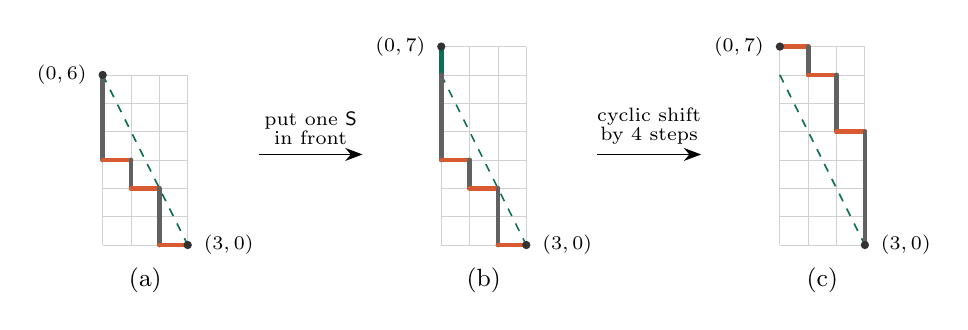
\begin{tikzpicture}
% fig_models.tex, generated by gen_figs.py of the guest session (Claude Fable 5.2 in the Claude app), 2026-11-14; inlined.
\draw[grid] (0.000,0.000) -- (0.000,2.160);
\draw[grid] (0.360,0.000) -- (0.360,2.160);
\draw[grid] (0.720,0.000) -- (0.720,2.160);
\draw[grid] (1.080,0.000) -- (1.080,2.160);
\draw[grid] (0.000,0.000) -- (1.080,0.000);
\draw[grid] (0.000,0.360) -- (1.080,0.360);
\draw[grid] (0.000,0.720) -- (1.080,0.720);
\draw[grid] (0.000,1.080) -- (1.080,1.080);
\draw[grid] (0.000,1.440) -- (1.080,1.440);
\draw[grid] (0.000,1.800) -- (1.080,1.800);
\draw[grid] (0.000,2.160) -- (1.080,2.160);
\draw[diag] (0.000,2.160) -- (1.080,0.000);
\draw[sstep] (0.000,2.160) -- (0.000,1.800);
\draw[sstep] (0.000,1.800) -- (0.000,1.440);
\draw[sstep] (0.000,1.440) -- (0.000,1.080);
\draw[estep] (0.000,1.080) -- (0.360,1.080);
\draw[sstep] (0.360,1.080) -- (0.360,0.720);
\draw[estep] (0.360,0.720) -- (0.720,0.720);
\draw[sstep] (0.720,0.720) -- (0.720,0.360);
\draw[sstep] (0.720,0.360) -- (0.720,0.000);
\draw[estep] (0.720,0.000) -- (1.080,0.000);
\fill[black!80] (0.000,2.160) circle (1.5pt);
\fill[black!80] (1.080,0.000) circle (1.5pt);
\node[font=\small] at (0.54,-0.45) {(a)};
\node[font=\scriptsize,anchor=east] at (-0.08,2.16) {$(0,6)$};
\node[font=\scriptsize,anchor=west] at (1.16,0) {$(3,0)$};
\draw[grid] (4.300,0.000) -- (4.300,2.520);
\draw[grid] (4.660,0.000) -- (4.660,2.520);
\draw[grid] (5.020,0.000) -- (5.020,2.520);
\draw[grid] (5.380,0.000) -- (5.380,2.520);
\draw[grid] (4.300,0.000) -- (5.380,0.000);
\draw[grid] (4.300,0.360) -- (5.380,0.360);
\draw[grid] (4.300,0.720) -- (5.380,0.720);
\draw[grid] (4.300,1.080) -- (5.380,1.080);
\draw[grid] (4.300,1.440) -- (5.380,1.440);
\draw[grid] (4.300,1.800) -- (5.380,1.800);
\draw[grid] (4.300,2.160) -- (5.380,2.160);
\draw[grid] (4.300,2.520) -- (5.380,2.520);
\draw[diag] (4.300,2.160) -- (5.380,0.000);
\draw[fstep] (4.300,2.520) -- (4.300,2.160);
\draw[sstep] (4.300,2.160) -- (4.300,1.800);
\draw[sstep] (4.300,1.800) -- (4.300,1.440);
\draw[sstep] (4.300,1.440) -- (4.300,1.080);
\draw[estep] (4.300,1.080) -- (4.660,1.080);
\draw[sstep] (4.660,1.080) -- (4.660,0.720);
\draw[estep] (4.660,0.720) -- (5.020,0.720);
\draw[sstep] (5.020,0.720) -- (5.020,0.360);
\draw[sstep] (5.020,0.360) -- (5.020,0.000);
\draw[estep] (5.020,0.000) -- (5.380,0.000);
\fill[black!80] (4.300,2.520) circle (1.5pt);
\fill[black!80] (5.380,0.000) circle (1.5pt);
\node[font=\small] at (4.84,-0.45) {(b)};
\node[font=\scriptsize,anchor=east] at (4.22,2.52) {$(0,7)$};
\node[font=\scriptsize,anchor=west] at (5.46,0) {$(3,0)$};
\draw[grid] (8.600,0.000) -- (8.600,2.520);
\draw[grid] (8.960,0.000) -- (8.960,2.520);
\draw[grid] (9.320,0.000) -- (9.320,2.520);
\draw[grid] (9.680,0.000) -- (9.680,2.520);
\draw[grid] (8.600,0.000) -- (9.680,0.000);
\draw[grid] (8.600,0.360) -- (9.680,0.360);
\draw[grid] (8.600,0.720) -- (9.680,0.720);
\draw[grid] (8.600,1.080) -- (9.680,1.080);
\draw[grid] (8.600,1.440) -- (9.680,1.440);
\draw[grid] (8.600,1.800) -- (9.680,1.800);
\draw[grid] (8.600,2.160) -- (9.680,2.160);
\draw[grid] (8.600,2.520) -- (9.680,2.520);
\draw[diag] (8.600,2.160) -- (9.680,0.000);
\draw[estep] (8.600,2.520) -- (8.960,2.520);
\draw[sstep] (8.960,2.520) -- (8.960,2.160);
\draw[estep] (8.960,2.160) -- (9.320,2.160);
\draw[sstep] (9.320,2.160) -- (9.320,1.800);
\draw[sstep] (9.320,1.800) -- (9.320,1.440);
\draw[estep] (9.320,1.440) -- (9.680,1.440);
\draw[sstep] (9.680,1.440) -- (9.680,1.080);
\draw[sstep] (9.680,1.080) -- (9.680,0.720);
\draw[sstep] (9.680,0.720) -- (9.680,0.360);
\draw[sstep] (9.680,0.360) -- (9.680,0.000);
\fill[black!80] (8.600,2.520) circle (1.5pt);
\fill[black!80] (9.680,0.000) circle (1.5pt);
\node[font=\small] at (9.14,-0.45) {(c)};
\node[font=\scriptsize,anchor=east] at (8.52,2.52) {$(0,7)$};
\node[font=\scriptsize,anchor=west] at (9.76,0) {$(3,0)$};
\draw[act] (1.98,1.15) -- node[above,font=\scriptsize,align=center]{put one \textsf{S}\\[-1pt] in front} (3.30,1.15);
\draw[act] (6.28,1.15) -- node[above,font=\scriptsize,align=center]{cyclic shift\\[-1pt] by $4$ steps} (7.60,1.15);
\end{tikzpicture}
\caption{$p=q=3$, $n=3$, so $m=7$, $N=10$, $C=12$. Steps $\E$ are drawn in coral, steps $\Ss$ in grey.
(a) A path from $(0,6)$ to $(3,0)$ under the dashed line. (b) The same path with one step $\Ss$ (teal) put in
front: a path in $\W$. (c) One of the other nine cyclic shifts of (b); none of them is of the form (b).
% Words added 2026-11-15 after the AI review of brief W053, read off the source of the picture; not in the text that was approved.
\revnote{in words: (a) is the path $\Ss\Ss\Ss\E\Ss\E\Ss\Ss\E$; (b) is $\Ss\Ss\Ss\Ss\E\Ss\E\Ss\Ss\E$; (c) is
$\E\Ss\E\Ss\Ss\E\Ss\Ss\Ss\Ss$, the cyclic shift of (b) by four steps.}}
\label{path:fig:models}
\end{figure}

\subsection{Segments, moves and classes}\label{path:sec:moves}

\emph{In Sections \ref{path:sec:moves}--\ref{path:sec:count}, $n,m\ge 0$ are arbitrary integers, $N=n+m$, and $\W$ is the set of words of length $N$
with $n$ letters $\E$ and $m$ letters $\Ss$. Only Section~\ref{path:sec:proof} uses $N=qn+1$.}

\paragraph{Segments.} Write $N=\sum_i N_ip^i$ in base $p$. Cut the positions $1,\dots,N$ into consecutive intervals:
$N_i$ intervals of length $p^i$ for each $i$, in order of decreasing length. These are the \emph{top segments}.
Cut every segment of length $p^h$, $h\ge1$, into $p$ consecutive \emph{sub-segments} of length $p^{h-1}$, and
repeat down to single steps. A \emph{segment} is a top segment or one of these iterated sub-segments.
The segments depend only on $N$ and $p$, not on the path. For a path $w$ and a segment $I$, the
\emph{piece} $w|_I$ is the part of $w$ on $I$.

When $N=qn+1$ the digits of $N$ are those of $n$, moved up by $k$ places, and a digit $1$ in place $0$:
\begin{equation}\label{path:eq:digitsN}
N_0=1,\qquad N_i=0\ \ (0<i<k),\qquad N_{k+i}=n_i .
\end{equation}
So there are $n_i$ top segments of length $q\,p^i$, followed by one single step.

\paragraph{Moves.} Let $I$ be a segment of length $p^h$, $h\ge 1$, and let $w|_I=u_1u_2\cdots u_p$, where $u_j$
is the piece on the $j$-th sub-segment. The \emph{move at $I$} replaces $u_1u_2\cdots u_p$ by $u_2\cdots u_pu_1$ and
changes nothing outside $I$. In words: cut this part of the path into $p$ equal pieces and glue them back in
rotated order (Figure~\ref{path:fig:moves}). A move permutes the steps, so it maps $\W$ to itself, and doing it $p$ times
gives back the path.

Two paths are \emph{equivalent} if a sequence of moves takes one to the other. All segments of length $p^h$ are
cut in the same way, so the same definition applies to words of length $p^h$: two such words $u,u'$ are
equivalent, $u\sim u'$, if, when they are placed on a segment $I$ of length $p^h$, moves at segments contained in $I$
take $u$ to $u'$. We write $[u]$ for the class of $u$, a set of words of length $p^h$. In particular we can
compare the pieces of a path on two different segments of the same length.

\begin{figure}[ht]
\centering
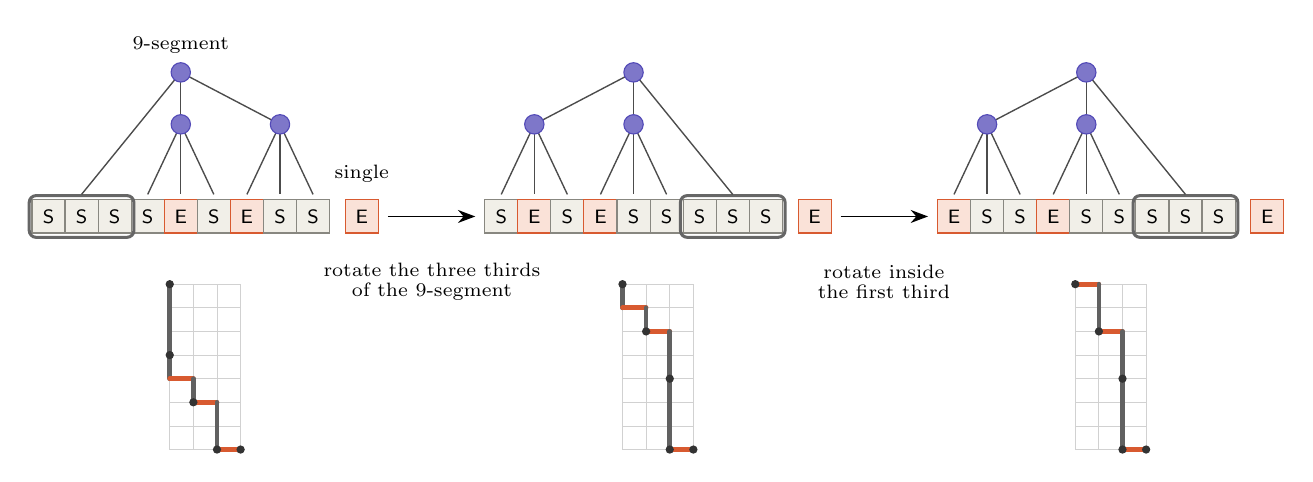
\begin{tikzpicture}
% fig_moves.tex, generated by gen_figs.py of the guest session (Claude Fable 5.2 in the Claude app), 2026-11-14; inlined.
\node[sbox] at (0.210,0.210) {\textsf{S}};
\node[sbox] at (0.630,0.210) {\textsf{S}};
\node[sbox] at (1.050,0.210) {\textsf{S}};
\node[sbox] at (1.470,0.210) {\textsf{S}};
\node[ebox] at (1.890,0.210) {\textsf{E}};
\node[sbox] at (2.310,0.210) {\textsf{S}};
\node[ebox] at (2.730,0.210) {\textsf{E}};
\node[sbox] at (3.150,0.210) {\textsf{S}};
\node[sbox] at (3.570,0.210) {\textsf{S}};
\node[ebox] at (4.190,0.210) {\textsf{E}};
\draw[satom] (-0.035,-0.055) rectangle (1.295,0.475);
\draw[edge] (1.890,2.040) -- (0.630,0.490);
\draw[edge] (1.890,2.040) -- (1.890,1.380);
\draw[edge] (1.890,1.380) -- (1.470,0.490);
\draw[edge] (1.890,1.380) -- (1.890,0.490);
\draw[edge] (1.890,1.380) -- (2.310,0.490);
\node[asymn] at (1.890,1.380) {};
\draw[edge] (1.890,2.040) -- (3.150,1.380);
\draw[edge] (3.150,1.380) -- (2.730,0.490);
\draw[edge] (3.150,1.380) -- (3.150,0.490);
\draw[edge] (3.150,1.380) -- (3.570,0.490);
\node[asymn] at (3.150,1.380) {};
\node[asymn] at (1.890,2.040) {};
\draw[grid] (1.750,-2.750) -- (1.750,-0.650);
\draw[grid] (2.050,-2.750) -- (2.050,-0.650);
\draw[grid] (2.350,-2.750) -- (2.350,-0.650);
\draw[grid] (2.650,-2.750) -- (2.650,-0.650);
\draw[grid] (1.750,-2.750) -- (2.650,-2.750);
\draw[grid] (1.750,-2.450) -- (2.650,-2.450);
\draw[grid] (1.750,-2.150) -- (2.650,-2.150);
\draw[grid] (1.750,-1.850) -- (2.650,-1.850);
\draw[grid] (1.750,-1.550) -- (2.650,-1.550);
\draw[grid] (1.750,-1.250) -- (2.650,-1.250);
\draw[grid] (1.750,-0.950) -- (2.650,-0.950);
\draw[grid] (1.750,-0.650) -- (2.650,-0.650);
\draw[sstep] (1.750,-0.650) -- (1.750,-0.950);
\draw[sstep] (1.750,-0.950) -- (1.750,-1.250);
\draw[sstep] (1.750,-1.250) -- (1.750,-1.550);
\draw[sstep] (1.750,-1.550) -- (1.750,-1.850);
\draw[estep] (1.750,-1.850) -- (2.050,-1.850);
\draw[sstep] (2.050,-1.850) -- (2.050,-2.150);
\draw[estep] (2.050,-2.150) -- (2.350,-2.150);
\draw[sstep] (2.350,-2.150) -- (2.350,-2.450);
\draw[sstep] (2.350,-2.450) -- (2.350,-2.750);
\draw[estep] (2.350,-2.750) -- (2.650,-2.750);
\fill[black!80] (1.750,-1.550) circle (1.5pt);
\fill[black!80] (2.050,-2.150) circle (1.5pt);
\fill[black!80] (2.350,-2.750) circle (1.5pt);
\fill[black!80] (1.750,-0.650) circle (1.5pt);
\fill[black!80] (2.650,-2.750) circle (1.5pt);
\node[sbox] at (5.960,0.210) {\textsf{S}};
\node[ebox] at (6.380,0.210) {\textsf{E}};
\node[sbox] at (6.800,0.210) {\textsf{S}};
\node[ebox] at (7.220,0.210) {\textsf{E}};
\node[sbox] at (7.640,0.210) {\textsf{S}};
\node[sbox] at (8.060,0.210) {\textsf{S}};
\node[sbox] at (8.480,0.210) {\textsf{S}};
\node[sbox] at (8.900,0.210) {\textsf{S}};
\node[sbox] at (9.320,0.210) {\textsf{S}};
\node[ebox] at (9.940,0.210) {\textsf{E}};
\draw[edge] (7.640,2.040) -- (6.380,1.380);
\draw[edge] (6.380,1.380) -- (5.960,0.490);
\draw[edge] (6.380,1.380) -- (6.380,0.490);
\draw[edge] (6.380,1.380) -- (6.800,0.490);
\node[asymn] at (6.380,1.380) {};
\draw[edge] (7.640,2.040) -- (7.640,1.380);
\draw[edge] (7.640,1.380) -- (7.220,0.490);
\draw[edge] (7.640,1.380) -- (7.640,0.490);
\draw[edge] (7.640,1.380) -- (8.060,0.490);
\node[asymn] at (7.640,1.380) {};
\draw[satom] (8.235,-0.055) rectangle (9.565,0.475);
\draw[edge] (7.640,2.040) -- (8.900,0.490);
\node[asymn] at (7.640,2.040) {};
\draw[grid] (7.500,-2.750) -- (7.500,-0.650);
\draw[grid] (7.800,-2.750) -- (7.800,-0.650);
\draw[grid] (8.100,-2.750) -- (8.100,-0.650);
\draw[grid] (8.400,-2.750) -- (8.400,-0.650);
\draw[grid] (7.500,-2.750) -- (8.400,-2.750);
\draw[grid] (7.500,-2.450) -- (8.400,-2.450);
\draw[grid] (7.500,-2.150) -- (8.400,-2.150);
\draw[grid] (7.500,-1.850) -- (8.400,-1.850);
\draw[grid] (7.500,-1.550) -- (8.400,-1.550);
\draw[grid] (7.500,-1.250) -- (8.400,-1.250);
\draw[grid] (7.500,-0.950) -- (8.400,-0.950);
\draw[grid] (7.500,-0.650) -- (8.400,-0.650);
\draw[sstep] (7.500,-0.650) -- (7.500,-0.950);
\draw[estep] (7.500,-0.950) -- (7.800,-0.950);
\draw[sstep] (7.800,-0.950) -- (7.800,-1.250);
\draw[estep] (7.800,-1.250) -- (8.100,-1.250);
\draw[sstep] (8.100,-1.250) -- (8.100,-1.550);
\draw[sstep] (8.100,-1.550) -- (8.100,-1.850);
\draw[sstep] (8.100,-1.850) -- (8.100,-2.150);
\draw[sstep] (8.100,-2.150) -- (8.100,-2.450);
\draw[sstep] (8.100,-2.450) -- (8.100,-2.750);
\draw[estep] (8.100,-2.750) -- (8.400,-2.750);
\fill[black!80] (7.800,-1.250) circle (1.5pt);
\fill[black!80] (8.100,-1.850) circle (1.5pt);
\fill[black!80] (8.100,-2.750) circle (1.5pt);
\fill[black!80] (7.500,-0.650) circle (1.5pt);
\fill[black!80] (8.400,-2.750) circle (1.5pt);
\node[ebox] at (11.710,0.210) {\textsf{E}};
\node[sbox] at (12.130,0.210) {\textsf{S}};
\node[sbox] at (12.550,0.210) {\textsf{S}};
\node[ebox] at (12.970,0.210) {\textsf{E}};
\node[sbox] at (13.390,0.210) {\textsf{S}};
\node[sbox] at (13.810,0.210) {\textsf{S}};
\node[sbox] at (14.230,0.210) {\textsf{S}};
\node[sbox] at (14.650,0.210) {\textsf{S}};
\node[sbox] at (15.070,0.210) {\textsf{S}};
\node[ebox] at (15.690,0.210) {\textsf{E}};
\draw[edge] (13.390,2.040) -- (12.130,1.380);
\draw[edge] (12.130,1.380) -- (11.710,0.490);
\draw[edge] (12.130,1.380) -- (12.130,0.490);
\draw[edge] (12.130,1.380) -- (12.550,0.490);
\node[asymn] at (12.130,1.380) {};
\draw[edge] (13.390,2.040) -- (13.390,1.380);
\draw[edge] (13.390,1.380) -- (12.970,0.490);
\draw[edge] (13.390,1.380) -- (13.390,0.490);
\draw[edge] (13.390,1.380) -- (13.810,0.490);
\node[asymn] at (13.390,1.380) {};
\draw[satom] (13.985,-0.055) rectangle (15.315,0.475);
\draw[edge] (13.390,2.040) -- (14.650,0.490);
\node[asymn] at (13.390,2.040) {};
\draw[grid] (13.250,-2.750) -- (13.250,-0.650);
\draw[grid] (13.550,-2.750) -- (13.550,-0.650);
\draw[grid] (13.850,-2.750) -- (13.850,-0.650);
\draw[grid] (14.150,-2.750) -- (14.150,-0.650);
\draw[grid] (13.250,-2.750) -- (14.150,-2.750);
\draw[grid] (13.250,-2.450) -- (14.150,-2.450);
\draw[grid] (13.250,-2.150) -- (14.150,-2.150);
\draw[grid] (13.250,-1.850) -- (14.150,-1.850);
\draw[grid] (13.250,-1.550) -- (14.150,-1.550);
\draw[grid] (13.250,-1.250) -- (14.150,-1.250);
\draw[grid] (13.250,-0.950) -- (14.150,-0.950);
\draw[grid] (13.250,-0.650) -- (14.150,-0.650);
\draw[estep] (13.250,-0.650) -- (13.550,-0.650);
\draw[sstep] (13.550,-0.650) -- (13.550,-0.950);
\draw[sstep] (13.550,-0.950) -- (13.550,-1.250);
\draw[estep] (13.550,-1.250) -- (13.850,-1.250);
\draw[sstep] (13.850,-1.250) -- (13.850,-1.550);
\draw[sstep] (13.850,-1.550) -- (13.850,-1.850);
\draw[sstep] (13.850,-1.850) -- (13.850,-2.150);
\draw[sstep] (13.850,-2.150) -- (13.850,-2.450);
\draw[sstep] (13.850,-2.450) -- (13.850,-2.750);
\draw[estep] (13.850,-2.750) -- (14.150,-2.750);
\fill[black!80] (13.550,-1.250) circle (1.5pt);
\fill[black!80] (13.850,-1.850) circle (1.5pt);
\fill[black!80] (13.850,-2.750) circle (1.5pt);
\fill[black!80] (13.250,-0.650) circle (1.5pt);
\fill[black!80] (14.150,-2.750) circle (1.5pt);
\draw[act] (4.52,0.21) -- (5.63,0.21);
\node[font=\scriptsize,align=center] at (5.08,-0.62) {rotate the three thirds\\[-1pt] of the $9$-segment};
\draw[act] (10.27,0.21) -- (11.38,0.21);
\node[font=\scriptsize,align=center] at (10.82,-0.62) {rotate inside\\[-1pt] the first third};
\node[font=\scriptsize,anchor=south] at (1.89,2.16) {$9$-segment};
\node[font=\scriptsize,anchor=south] at (4.19,0.52) {single};
\end{tikzpicture}
\caption{$p=3$, $N=10$: one top segment of length $9$ and one single step. Top row: the path (b) of
Figure~\ref{path:fig:models} as a word, with its segments drawn as a tree, and two moves. A box drawn around several steps
is a monochromatic segment; purple discs are asymmetric segments (Definition~\ref{path:def:sym}). All three paths have
$d=3$. Bottom row: the same three paths in the plane; the dots cut the $9$-segment into thirds.
% Words added 2026-11-15 after the AI review of brief W053, read off the source of the picture; not in the text that was approved.
\revnote{in words, the three paths are, from left to right: $\Ss\Ss\Ss\,\Ss\E\Ss\,\E\Ss\Ss\,\E$; then, after
the move at the $9$-segment, which turns its thirds $\Ss\Ss\Ss$, $\Ss\E\Ss$, $\E\Ss\Ss$ into $\Ss\E\Ss$,
$\E\Ss\Ss$, $\Ss\Ss\Ss$, the path $\Ss\E\Ss\,\E\Ss\Ss\,\Ss\Ss\Ss\,\E$; then, after the move at the first
third, which turns $\Ss\E\Ss$ into $\E\Ss\Ss$, the path $\E\Ss\Ss\,\E\Ss\Ss\,\Ss\Ss\Ss\,\E$. In each the last
letter is the single step.}}
\label{path:fig:moves}
\end{figure}

\begin{remark}
The moves generate a group of permutations of the $N$ positions: a product, over the top segments, of
iterated wreath products $\mathbb Z_p\wr\cdots\wr\mathbb Z_p$. It is the group of rotations of a forest of complete $p$-ary
trees whose leaves are the steps of the path. The classes are its orbits. By \cite[p.~239]{Kaloujnine} and
\cite[Section~2]{GiannelliLaw} (odd $p$ there), as recorded in the project's \texttt{references/README.md}, this group is a Sylow
$p$-subgroup of the symmetric group of the $N$ positions. We only need the classes.
\end{remark}

\begin{definition}\label{path:def:sym}
A piece is \emph{monochromatic} if all its steps are equal, and \emph{mixed} otherwise; we use the same words
for the segment carrying it. A segment $I$ of length $p^h$, $h\ge1$, is \emph{symmetric} for $w$ if the $p$
pieces of $w$ on its sub-segments are equivalent to one another, and \emph{asymmetric} otherwise. Single
steps count as symmetric. Monochromatic segments are symmetric. For a piece $u$ on a segment $I$, let $d(u)$ be the number of asymmetric segments contained in $I$, with $I$
itself; it depends only on the word $u$. For a path $w$, let $d(w)=\sum_Td(w|_T)$, the sum over the top segments
$T$: the number of all asymmetric segments.
\end{definition}

\begin{lemma}\label{path:lem:classes}
Let $I$ be a segment of length $p^h$, $h\ge 1$, and $u=u_1\cdots u_p$, $u'=u'_1\cdots u'_p$ two pieces on $I$.
Then $u\sim u'$ if and only if there is an $r$ with $u'_j\sim u_{j+r}$ for all $j$ (indices modulo $p$).
\end{lemma}
\begin{proof}
A move at a segment inside $I$ is either the move at $I$, which rotates the sequence of classes
$([u_1],\dots,[u_p])$, or a move inside one sub-segment, which does not change this sequence. So the
sequence of classes is determined by the class of $u$ up to rotation. Conversely, if $u'_j\sim u_{j+r}$ for all
$j$, apply the move at $I$ $r$ times and then moves inside the sub-segments.
\end{proof}

\begin{lemma}[class sizes]\label{path:lem:size}
The class of a piece $u$ has exactly $p^{\,d(u)}$ elements. The class of a path $w$ has
exactly $p^{\,d(w)}$ elements. In particular $d$ is constant on classes.
\end{lemma}
\begin{proof}
Let $u=u_1\cdots u_p$ be on a segment $I$ of length $p^h$. Induction on $h$; for $h=0$ both sides are $1$. Let $h\ge 1$. By Lemma~\ref{path:lem:classes},
$[u]$ is the union, over $r=0,\dots,p-1$, of the sets of words $v_1\cdots v_p$ with $v_j\in[u_{j+r}]$.
If $I$ is symmetric these $p$ sets coincide, so $|[u]|=\prod_j|[u_j]|$. If $I$ is asymmetric, the $p$ rotations
of the sequence $([u_1],\dots,[u_p])$ are pairwise distinct, because $p$ is prime and the sequence is not constant;
so the $p$ sets are disjoint and $|[u]|=p\prod_j|[u_j]|$. By induction $|[u_j]|=p^{d(u_j)}$, and
$d(u)=\sum_j d(u_j)$, plus $1$ if $I$ is asymmetric.
Finally, every move acts inside one top segment, so the class of $w$ is the product of the classes of its top pieces.
\end{proof}

\begin{figure}[ht]
\centering
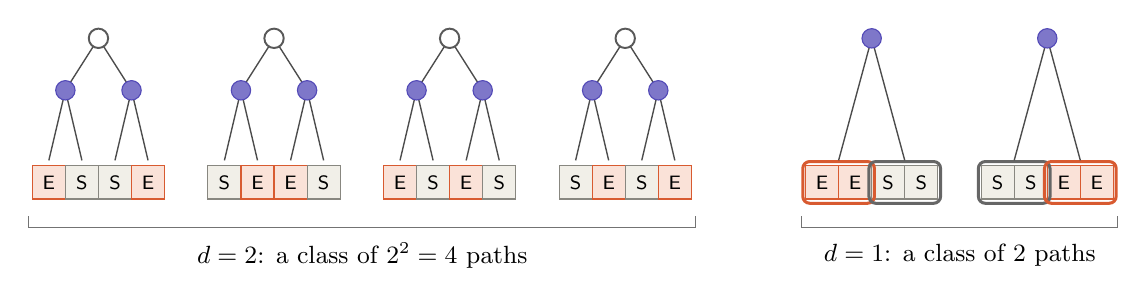
\begin{tikzpicture}
% fig_classes.tex, generated by gen_figs.py of the guest session (Claude Fable 5.2 in the Claude app), 2026-11-14; inlined.
\node[ebox] at (0.210,0.210) {\textsf{E}};
\node[sbox] at (0.630,0.210) {\textsf{S}};
\node[sbox] at (1.050,0.210) {\textsf{S}};
\node[ebox] at (1.470,0.210) {\textsf{E}};
\draw[edge] (0.840,2.040) -- (0.420,1.380);
\draw[edge] (0.420,1.380) -- (0.210,0.490);
\draw[edge] (0.420,1.380) -- (0.630,0.490);
\node[asymn] at (0.420,1.380) {};
\draw[edge] (0.840,2.040) -- (1.260,1.380);
\draw[edge] (1.260,1.380) -- (1.050,0.490);
\draw[edge] (1.260,1.380) -- (1.470,0.490);
\node[asymn] at (1.260,1.380) {};
\node[symn] at (0.840,2.040) {};
\node[sbox] at (2.440,0.210) {\textsf{S}};
\node[ebox] at (2.860,0.210) {\textsf{E}};
\node[ebox] at (3.280,0.210) {\textsf{E}};
\node[sbox] at (3.700,0.210) {\textsf{S}};
\draw[edge] (3.070,2.040) -- (2.650,1.380);
\draw[edge] (2.650,1.380) -- (2.440,0.490);
\draw[edge] (2.650,1.380) -- (2.860,0.490);
\node[asymn] at (2.650,1.380) {};
\draw[edge] (3.070,2.040) -- (3.490,1.380);
\draw[edge] (3.490,1.380) -- (3.280,0.490);
\draw[edge] (3.490,1.380) -- (3.700,0.490);
\node[asymn] at (3.490,1.380) {};
\node[symn] at (3.070,2.040) {};
\node[ebox] at (4.670,0.210) {\textsf{E}};
\node[sbox] at (5.090,0.210) {\textsf{S}};
\node[ebox] at (5.510,0.210) {\textsf{E}};
\node[sbox] at (5.930,0.210) {\textsf{S}};
\draw[edge] (5.300,2.040) -- (4.880,1.380);
\draw[edge] (4.880,1.380) -- (4.670,0.490);
\draw[edge] (4.880,1.380) -- (5.090,0.490);
\node[asymn] at (4.880,1.380) {};
\draw[edge] (5.300,2.040) -- (5.720,1.380);
\draw[edge] (5.720,1.380) -- (5.510,0.490);
\draw[edge] (5.720,1.380) -- (5.930,0.490);
\node[asymn] at (5.720,1.380) {};
\node[symn] at (5.300,2.040) {};
\node[sbox] at (6.900,0.210) {\textsf{S}};
\node[ebox] at (7.320,0.210) {\textsf{E}};
\node[sbox] at (7.740,0.210) {\textsf{S}};
\node[ebox] at (8.160,0.210) {\textsf{E}};
\draw[edge] (7.530,2.040) -- (7.110,1.380);
\draw[edge] (7.110,1.380) -- (6.900,0.490);
\draw[edge] (7.110,1.380) -- (7.320,0.490);
\node[asymn] at (7.110,1.380) {};
\draw[edge] (7.530,2.040) -- (7.950,1.380);
\draw[edge] (7.950,1.380) -- (7.740,0.490);
\draw[edge] (7.950,1.380) -- (8.160,0.490);
\node[asymn] at (7.950,1.380) {};
\node[symn] at (7.530,2.040) {};
\draw[brace] (-0.05,-0.22) -- (-0.05,-0.36) -- (8.42,-0.36) -- (8.42,-0.22);
\node[font=\small] at (4.19,-0.72) {$d=2$: a class of $2^2=4$ paths};
\node[ebox] at (10.030,0.210) {\textsf{E}};
\node[ebox] at (10.450,0.210) {\textsf{E}};
\node[sbox] at (10.870,0.210) {\textsf{S}};
\node[sbox] at (11.290,0.210) {\textsf{S}};
\draw[eatom] (9.785,-0.055) rectangle (10.695,0.475);
\draw[edge] (10.660,2.040) -- (10.240,0.490);
\draw[satom] (10.625,-0.055) rectangle (11.535,0.475);
\draw[edge] (10.660,2.040) -- (11.080,0.490);
\node[asymn] at (10.660,2.040) {};
\node[sbox] at (12.260,0.210) {\textsf{S}};
\node[sbox] at (12.680,0.210) {\textsf{S}};
\node[ebox] at (13.100,0.210) {\textsf{E}};
\node[ebox] at (13.520,0.210) {\textsf{E}};
\draw[satom] (12.015,-0.055) rectangle (12.925,0.475);
\draw[edge] (12.890,2.040) -- (12.470,0.490);
\draw[eatom] (12.855,-0.055) rectangle (13.765,0.475);
\draw[edge] (12.890,2.040) -- (13.310,0.490);
\node[asymn] at (12.890,2.040) {};
\draw[brace] (9.77,-0.22) -- (9.77,-0.36) -- (13.78,-0.36) -- (13.78,-0.22);
\node[font=\small] at (11.78,-0.72) {$d=1$: a class of $2$ paths};
\end{tikzpicture}
\caption{$p=2$, one segment of length $4$, all $\binom42=6$ paths with two steps $\E$ and two steps $\Ss$.
Purple discs: asymmetric segments. White circles: symmetric mixed segments. In the class on the left the two halves
differ, but each half is a rotation of the other, so the whole segment is symmetric.
Here $6=2+4$: the lower bound of Section~\ref{path:sec:bound} is $d\ge1$, and there is one minimal class. \assembler{in words, the class of size $2$ is $\{\E\E\Ss\Ss,\ \Ss\Ss\E\E\}$ (both halves monochromatic, the
whole segment asymmetric, $d=1$), and the class of size $4$ is
$\{\E\Ss\E\Ss,\ \E\Ss\Ss\E,\ \Ss\E\E\Ss,\ \Ss\E\Ss\E\}$ (both halves asymmetric, the whole segment symmetric,
$d=2$).}}
\label{path:fig:classes}
\end{figure}

\begin{corollary}\label{path:cor:sum}
$\displaystyle\binom Nn=|\W|=\sum_{\text{classes}}p^{\,d}$, where $d$ is the common value of $d(w)$ on the class.
\end{corollary}

\subsection{A lower bound from digit sums}\label{path:sec:bound}

\begin{lemma}[carries]\label{path:lem:carries}
Define $c_0=0$ and $c_{i+1}=(n_i+m_i+c_i-N_i)/p$ for $i\ge 0$. Then every $c_i$ is $0$ or $1$, and
\[
c:=\sum_i c_i=\frac{s_p(n)+s_p(m)-s_p(N)}{p-1}.
\]
\end{lemma}
\begin{proof}
For an integer $u$ let $u^{(i)}$ be its remainder modulo $p^i$. Put $c'_i=(n^{(i)}+m^{(i)}-N^{(i)})/p^i$. This is an
integer, since $n+m=N$; it is $0$ or $1$, since $0\le n^{(i)}+m^{(i)}\le 2p^i-2$ and $0\le N^{(i)}\le p^i-1$.
Subtracting the definitions for $i$ and $i+1$ gives $n_i+m_i+c'_i=N_i+p\,c'_{i+1}$, and $c'_0=0$. So $c'_i=c_i$ for
all $i$. Summing $n_i+m_i+c_i=N_i+p\,c_{i+1}$ over $i$
(all $c_i$ with $p^i>N$ vanish) gives $s_p(n)+s_p(m)+c=s_p(N)+p\,c$.
\end{proof}

The number $c_i$ is the carry into digit $i$ when $n$ and $m$ are added in base $p$, and $c$ is the number of
carries.
% Clarification added 2026-11-15 after the referee report (report/reviews/REFEREE.md, finding 11); not in the text that was approved.
\refnote{in Lemma~\ref{main:lem:digit} of the main proof $c_j$ is the carry \emph{out of} column $j$, which is
$c_{j+1}$ in the notation used here; and in Section~\ref{sec:mainproof} the letter $c$ also denotes a depth
class in $\Z_k$.}
We say that integers $u^1,\dots,u^r\ge0$ \emph{add without carries} if in every digit place $i$ the sum of
their digits $\sum_j (u^j)_i$ is at most $p-1$; this sum is then the $i$-th digit of $u^1+\dots+u^r$.

\begin{lemma}[digit sums]\label{path:lem:digits}
\textup{(a)} $s_p(pu)=s_p(u)$. \textup{(b)} $s_p(u^1+\dots+u^r)\le s_p(u^1)+\dots+s_p(u^r)$, with equality
exactly when $u^1,\dots,u^r$ add without carries.
\end{lemma}
\begin{proof}
(a) is clear. For $r=2$, (b) is Lemma~\ref{path:lem:carries}: the difference of the two sides is $(p-1)c\ge0$, and $c=0$
exactly when $n_i+m_i\le p-1$ for all $i$. The general case follows by induction on $r$, adding one summand at a time.
\end{proof}

For a piece $u$ on a segment of length $p^h$ let $a(u)$ and $b(u)$ be its numbers of steps $\E$ and $\Ss$, so
$a(u)+b(u)=p^h$, and put
\[
\tau(u)=\frac{s_p(a(u))+s_p(b(u))-1}{p-1}.
\]

\begin{lemma}[lower bound for a piece]\label{path:lem:bound}
Let $u$ be a piece on a segment $I$, with sub-pieces $u_1,\dots,u_p$ if $I$ is longer than one step. Then
$d(u)\ge\tau(u)$. Equality holds exactly when either
$u$ is monochromatic, or the following three conditions hold: $I$ is asymmetric; equality holds for every
$u_j$; and $a(u_1),\dots,a(u_p)$ add without carries, and so do $b(u_1),\dots,b(u_p)$.
\end{lemma}
\begin{proof}
Induction on the length of $I$. Three cases.

\emph{$u$ monochromatic.} Then $d(u)=0$, and $\tau(u)=(0+s_p(p^h)-1)/(p-1)=0$.

\emph{$u$ mixed, $I$ symmetric.} The $u_j$ are equivalent to one another, so they have the same $a$, $b$ and $d$
(Lemma~\ref{path:lem:size}): $a(u)=p\,a(u_1)$, $b(u)=p\,b(u_1)$ and $d(u)=p\,d(u_1)$. As $u_1$ is mixed,
$\tau(u_1)>0$. So
\[
d(u)=p\,d(u_1)\ \ge\ p\,\tau(u_1)\ >\ \tau(u_1)=\tau(u),
\]
the last equality by Lemma~\ref{path:lem:digits}(a). Equality never holds in this case.

\emph{$I$ asymmetric.} Then, by induction and Lemma~\ref{path:lem:digits}(b),
\begin{align*}
d(u)=1+\sum_j d(u_j)\ &\ge\ 1+\sum_j\tau(u_j)
=1+\frac{\sum_j s_p(a(u_j))+\sum_j s_p(b(u_j))-p}{p-1}\\
&\ge\ 1+\frac{s_p(a(u))+s_p(b(u))-p}{p-1}=\tau(u),
\end{align*}
with equality exactly under the stated conditions.
\end{proof}

\begin{proposition}[lower bound]\label{path:prop:bound}
For every path $w\in\W$, $d(w)\ge c$, the number of carries. Equality holds exactly when equality holds in
Lemma~\ref{path:lem:bound} for every top piece, the numbers $a(w|_T)$ over the top segments $T$ add without carries,
and so do the numbers $b(w|_T)$.
\end{proposition}
\begin{proof}
There are $\sum_iN_i=s_p(N)$ top segments, $\sum_Ta(w|_T)=n$ and $\sum_Tb(w|_T)=m$. So by
Lemmas \ref{path:lem:bound} and \ref{path:lem:digits}(b),
\begin{align*}
d(w)=\sum_T d(w|_T)\ &\ge\ \sum_T\tau(w|_T)=\frac{\sum_Ts_p(a(w|_T))+\sum_Ts_p(b(w|_T))-s_p(N)}{p-1}\\
&\ge\ \frac{s_p(n)+s_p(m)-s_p(N)}{p-1}=c. \qedhere
\end{align*}
\end{proof}

We call $w$ \emph{minimal} if $d(w)=c$. By Lemma~\ref{path:lem:size} a class consists of minimal paths or contains
none. Corollary~\ref{path:cor:sum} and Proposition~\ref{path:prop:bound} give
\begin{equation}\label{path:eq:modp}
\binom Nn\;=\;p^{\,c}\,M+p^{\,c+1}R,\qquad M=\text{the number of classes of minimal paths},
\end{equation}
for some integer $R\ge0$. In particular $p^c$ divides $\binom Nn$.

\subsection{Minimal paths: atoms and carries}\label{path:sec:minimal}

\begin{definition}
An \emph{atom} of $w$ is a monochromatic segment that is a top segment or a sub-segment of a mixed segment. It is an
$\E$-atom or an $\Ss$-atom according to its steps. Every step of $w$ lies in exactly one atom: the largest
monochromatic segment containing it.
\end{definition}

\begin{lemma}[atoms are digits]\label{path:lem:atoms}
Let $w$ be minimal. Then every mixed segment is asymmetric, and for every $i$ the path $w$ has exactly $n_i$
$\E$-atoms and exactly $m_i$ $\Ss$-atoms of length $p^i$.
\end{lemma}
\begin{proof}
The first statement is part of the equality conditions of Lemma~\ref{path:lem:bound}, applied down the tree of segments. For the second, we show by induction
that for a piece $u$ with equality in Lemma~\ref{path:lem:bound}, the number of $\E$-atoms of length $p^i$ inside it is the
$i$-th digit of $a(u)$. If $u$ is monochromatic this is clear. If not, the atoms of $u$ are the atoms of
$u_1,\dots,u_p$, and the digits of $a(u_1),\dots,a(u_p)$ add up to the digits of $a(u)$ because these numbers
add without carries. The same argument at the top level (Proposition~\ref{path:prop:bound}) gives the digits of $n$, and the
same for $\Ss$ and $m$.
\end{proof}

\begin{lemma}[mixed segments are carries]\label{path:lem:mixed}
Let $w$ be minimal. For every $i$, the number of mixed segments of length $p^i$ is $c_i$. So $w$ has at most
one mixed segment of each length, and a mixed segment of length $p^i$ exactly when the addition $n+m=N$ carries
into digit $i$.
\end{lemma}
\begin{proof}
Let $x_i$ be the number of mixed segments of length $p^i$; $x_0=0$. Let $\mathcal R_i$ be the set of segments of
length $p^i$ that are top segments or sub-segments of a mixed segment. Then $|\mathcal R_i|=N_i+p\,x_{i+1}$. A member
of $\mathcal R_i$ is monochromatic, and then an atom, or mixed; and every atom and every mixed segment of length
$p^i$ lies in $\mathcal R_i$. By Lemma~\ref{path:lem:atoms},
\[
N_i+p\,x_{i+1}=n_i+m_i+x_i\qquad(i\ge0),\qquad x_0=0 .
\]
This is the recursion of Lemma~\ref{path:lem:carries}, so $x_i=c_i$ for all $i$.
\end{proof}

\subsection{Counting the minimal classes}\label{path:sec:count}

\begin{proposition}[count]\label{path:prop:count}
The number of minimal paths is $\prod_i\dfrac{(N_i+p\,c_{i+1})!}{n_i!\,m_i!}$. They form $M$ classes of $p^c$
paths each, where
\begin{equation}\label{path:eq:M}
M\cdot\prod_i n_i!\,m_i!\;=\;\prod_i\frac{(N_i+p\,c_{i+1})!}{p^{\,c_{i+1}}}\;\equiv\;(-1)^c\prod_iN_i!\pmod p .
\end{equation}
\end{proposition}
\begin{proof}
Build a minimal path from the longest segments down. By Lemma~\ref{path:lem:mixed} and its proof, at level $i$ there are
$N_i+p\,c_{i+1}$ \emph{slots}: the $N_i$ top segments of length $p^i$ and, if $c_{i+1}=1$, the $p$ sub-segments of
the unique mixed segment of length $p^{i+1}$, which was chosen at level $i+1$. Among the slots we choose $n_i$
to be $\E$-atoms, $m_i$ to be $\Ss$-atoms, and, if $c_i=1$, the remaining one to be mixed. The number of slots is
$n_i+m_i+c_i$, so this can be done in $(N_i+p\,c_{i+1})!/(n_i!\,m_i!)$ ways, whatever was chosen before.
At level $0$ there is nothing mixed, so the choices determine a word; it has $\sum_in_ip^i=n$ letters $\E$.

Every minimal path arises from exactly one sequence of choices (Lemmas \ref{path:lem:atoms} and \ref{path:lem:mixed}).
Conversely, let $w$ be built from any sequence of choices. The $p$ sub-segments of a segment chosen to be mixed
are slots of the next level; at most $n_{i-1}\le p-1$ of them are $\E$-atoms, at most $m_{i-1}\le p-1$ are
$\Ss$-atoms, and at most one is mixed. So its $p$ pieces are not all $\E$-atoms and not all $\Ss$-atoms. Going up from level $1$, this shows that a
segment chosen to be mixed really contains both letters. It is asymmetric: $p$ equivalent pieces
would be all monochromatic with the same letter, or all mixed, and both are excluded. All other segments are
monochromatic. Hence
$d(w)=\sum_ic_i=c$ and $w$ is minimal.

This proves the count of minimal paths. Each class of minimal paths has $p^c=\prod_ip^{c_{i+1}}$ elements
(Lemma~\ref{path:lem:size}), which gives the equality in \eqref{path:eq:M}. For the congruence: if $c_{i+1}=0$ the $i$-th
factor is $N_i!$. If $c_{i+1}=1$ it is
\[
\frac{(N_i+p)!}{p}=(p-1)!\,\prod_{j=1}^{N_i}(p+j)\;\equiv\;(p-1)!\,N_i!\;\equiv\;-N_i!\pmod p
\]
by Wilson's theorem.
\end{proof}

Together with \eqref{path:eq:modp} this gives the result for all binomial coefficients:

\begin{theorem}\label{path:thm:binom}
Let $n,m\ge0$, $N=n+m$, and let $c$ be the number of carries when $n$ and $m$ are added in base $p$. Then
$p^c$ divides $\binom Nn$ and
\[
\frac1{p^c}\binom Nn\;\equiv\;(-1)^c\prod_i\frac{N_i!}{n_i!\,m_i!}\pmod p .
\]
The right-hand side is not $0$ modulo $p$, so $p^c$ is the exact power of $p$ dividing $\binom Nn$.
\end{theorem}

\subsection{Proof of Theorem \ref{path:thm:main}}\label{path:sec:proof}

Let $N=qn+1$ and $m=(q-1)n+1$. By \eqref{path:eq:digitsN}, $s_p(N)=s_p(n)+1$ and $\prod_iN_i!=\prod_in_i!$. So the
number of carries is
\[
c=\frac{s_p(n)+s_p(m)-s_p(N)}{p-1}=\frac{s_p(m)-1}{p-1}=t ,
\]
and Theorem~\ref{path:thm:binom} gives $\binom Nn=p^tM+p^{t+1}R$ with $M\prod_jm_j!\equiv(-1)^t\pmod p$. By
Lemma~\ref{path:lem:shift}, $\binom Nn=N\cdot C$. As $p$ does not divide $N$, $p^t$ divides $C$. And as $N\equiv1\pmod p$,
\[
\frac C{p^t}\;\equiv\;\frac{N\cdot C}{p^t}\;\equiv\;M\;\equiv\;\frac{(-1)^t}{\prod_jm_j!}\pmod p. \qed
\]

\subsection{Two examples}

\begin{example}[$p=q=3$, $n=3$]\label{path:ex:A}
Here $m=7=(21)_3$, $N=10=(101)_3$, $C=12$ and $t=(3-1)/2=1$. The top segments are one segment of length $9$
and one single step. Adding $n=(10)_3$ and $m=(21)_3$ carries once, into digit $2$. So a minimal path has
one mixed segment, the $9$-segment. Its atoms are one $\E$-atom of length $3$ (the digits of $n$), and two
$\Ss$-atoms of length $3$ and one of length $1$ (the digits of $m$). The three thirds of the $9$-segment can be
filled in $3!/(1!\,2!)=3$ ways, and the single step is $\Ss$. These three paths form the only minimal class:
$M=1$ (Figure~\ref{path:fig:exA}).

All $\binom{10}3=120$ paths: one class of $3$, one class of $9$, four classes of $27$. So
$10\cdot C=120=3\cdot1+9\cdot13$, hence $C=12=3\cdot 4$ and $4\equiv1\equiv-1/(2!\,1!)\pmod 3$.
\end{example}

\begin{figure}[ht]
\centering
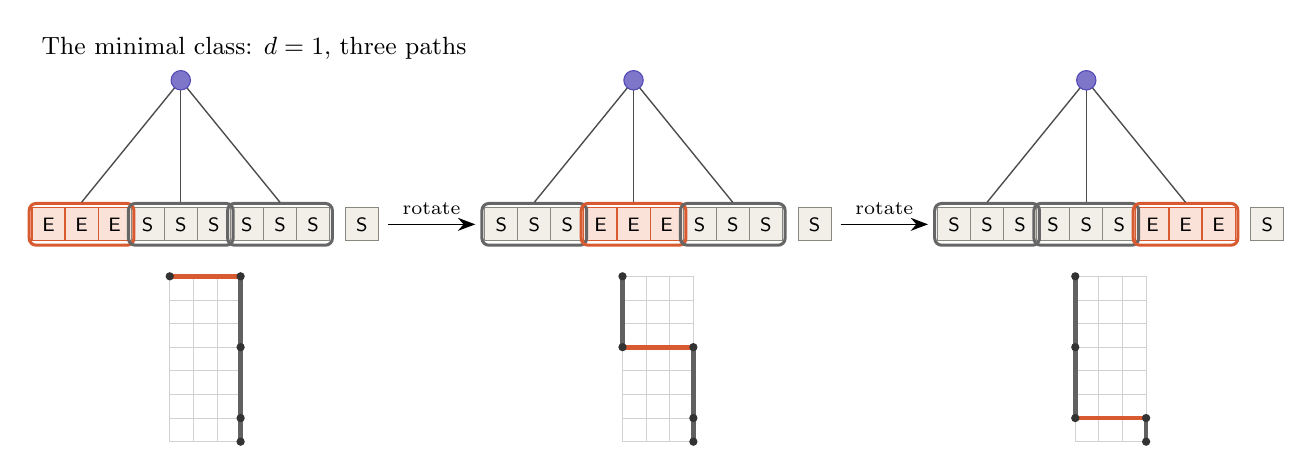
\begin{tikzpicture}
% fig_exA_min.tex, generated by gen_figs.py of the guest session (Claude Fable 5.2 in the Claude app), 2026-11-14; inlined.
\node[ebox] at (0.210,0.210) {\textsf{E}};
\node[ebox] at (0.630,0.210) {\textsf{E}};
\node[ebox] at (1.050,0.210) {\textsf{E}};
\node[sbox] at (1.470,0.210) {\textsf{S}};
\node[sbox] at (1.890,0.210) {\textsf{S}};
\node[sbox] at (2.310,0.210) {\textsf{S}};
\node[sbox] at (2.730,0.210) {\textsf{S}};
\node[sbox] at (3.150,0.210) {\textsf{S}};
\node[sbox] at (3.570,0.210) {\textsf{S}};
\node[sbox] at (4.190,0.210) {\textsf{S}};
\draw[eatom] (-0.035,-0.055) rectangle (1.295,0.475);
\draw[edge] (1.890,2.040) -- (0.630,0.490);
\draw[satom] (1.225,-0.055) rectangle (2.555,0.475);
\draw[edge] (1.890,2.040) -- (1.890,0.490);
\draw[satom] (2.485,-0.055) rectangle (3.815,0.475);
\draw[edge] (1.890,2.040) -- (3.150,0.490);
\node[asymn] at (1.890,2.040) {};
\draw[grid] (1.750,-2.550) -- (1.750,-0.450);
\draw[grid] (2.050,-2.550) -- (2.050,-0.450);
\draw[grid] (2.350,-2.550) -- (2.350,-0.450);
\draw[grid] (2.650,-2.550) -- (2.650,-0.450);
\draw[grid] (1.750,-2.550) -- (2.650,-2.550);
\draw[grid] (1.750,-2.250) -- (2.650,-2.250);
\draw[grid] (1.750,-1.950) -- (2.650,-1.950);
\draw[grid] (1.750,-1.650) -- (2.650,-1.650);
\draw[grid] (1.750,-1.350) -- (2.650,-1.350);
\draw[grid] (1.750,-1.050) -- (2.650,-1.050);
\draw[grid] (1.750,-0.750) -- (2.650,-0.750);
\draw[grid] (1.750,-0.450) -- (2.650,-0.450);
\draw[estep] (1.750,-0.450) -- (2.050,-0.450);
\draw[estep] (2.050,-0.450) -- (2.350,-0.450);
\draw[estep] (2.350,-0.450) -- (2.650,-0.450);
\draw[sstep] (2.650,-0.450) -- (2.650,-0.750);
\draw[sstep] (2.650,-0.750) -- (2.650,-1.050);
\draw[sstep] (2.650,-1.050) -- (2.650,-1.350);
\draw[sstep] (2.650,-1.350) -- (2.650,-1.650);
\draw[sstep] (2.650,-1.650) -- (2.650,-1.950);
\draw[sstep] (2.650,-1.950) -- (2.650,-2.250);
\draw[sstep] (2.650,-2.250) -- (2.650,-2.550);
\fill[black!80] (2.650,-0.450) circle (1.5pt);
\fill[black!80] (2.650,-1.350) circle (1.5pt);
\fill[black!80] (2.650,-2.250) circle (1.5pt);
\fill[black!80] (1.750,-0.450) circle (1.5pt);
\fill[black!80] (2.650,-2.550) circle (1.5pt);
\node[sbox] at (5.960,0.210) {\textsf{S}};
\node[sbox] at (6.380,0.210) {\textsf{S}};
\node[sbox] at (6.800,0.210) {\textsf{S}};
\node[ebox] at (7.220,0.210) {\textsf{E}};
\node[ebox] at (7.640,0.210) {\textsf{E}};
\node[ebox] at (8.060,0.210) {\textsf{E}};
\node[sbox] at (8.480,0.210) {\textsf{S}};
\node[sbox] at (8.900,0.210) {\textsf{S}};
\node[sbox] at (9.320,0.210) {\textsf{S}};
\node[sbox] at (9.940,0.210) {\textsf{S}};
\draw[satom] (5.715,-0.055) rectangle (7.045,0.475);
\draw[edge] (7.640,2.040) -- (6.380,0.490);
\draw[eatom] (6.975,-0.055) rectangle (8.305,0.475);
\draw[edge] (7.640,2.040) -- (7.640,0.490);
\draw[satom] (8.235,-0.055) rectangle (9.565,0.475);
\draw[edge] (7.640,2.040) -- (8.900,0.490);
\node[asymn] at (7.640,2.040) {};
\draw[grid] (7.500,-2.550) -- (7.500,-0.450);
\draw[grid] (7.800,-2.550) -- (7.800,-0.450);
\draw[grid] (8.100,-2.550) -- (8.100,-0.450);
\draw[grid] (8.400,-2.550) -- (8.400,-0.450);
\draw[grid] (7.500,-2.550) -- (8.400,-2.550);
\draw[grid] (7.500,-2.250) -- (8.400,-2.250);
\draw[grid] (7.500,-1.950) -- (8.400,-1.950);
\draw[grid] (7.500,-1.650) -- (8.400,-1.650);
\draw[grid] (7.500,-1.350) -- (8.400,-1.350);
\draw[grid] (7.500,-1.050) -- (8.400,-1.050);
\draw[grid] (7.500,-0.750) -- (8.400,-0.750);
\draw[grid] (7.500,-0.450) -- (8.400,-0.450);
\draw[sstep] (7.500,-0.450) -- (7.500,-0.750);
\draw[sstep] (7.500,-0.750) -- (7.500,-1.050);
\draw[sstep] (7.500,-1.050) -- (7.500,-1.350);
\draw[estep] (7.500,-1.350) -- (7.800,-1.350);
\draw[estep] (7.800,-1.350) -- (8.100,-1.350);
\draw[estep] (8.100,-1.350) -- (8.400,-1.350);
\draw[sstep] (8.400,-1.350) -- (8.400,-1.650);
\draw[sstep] (8.400,-1.650) -- (8.400,-1.950);
\draw[sstep] (8.400,-1.950) -- (8.400,-2.250);
\draw[sstep] (8.400,-2.250) -- (8.400,-2.550);
\fill[black!80] (7.500,-1.350) circle (1.5pt);
\fill[black!80] (8.400,-1.350) circle (1.5pt);
\fill[black!80] (8.400,-2.250) circle (1.5pt);
\fill[black!80] (7.500,-0.450) circle (1.5pt);
\fill[black!80] (8.400,-2.550) circle (1.5pt);
\node[sbox] at (11.710,0.210) {\textsf{S}};
\node[sbox] at (12.130,0.210) {\textsf{S}};
\node[sbox] at (12.550,0.210) {\textsf{S}};
\node[sbox] at (12.970,0.210) {\textsf{S}};
\node[sbox] at (13.390,0.210) {\textsf{S}};
\node[sbox] at (13.810,0.210) {\textsf{S}};
\node[ebox] at (14.230,0.210) {\textsf{E}};
\node[ebox] at (14.650,0.210) {\textsf{E}};
\node[ebox] at (15.070,0.210) {\textsf{E}};
\node[sbox] at (15.690,0.210) {\textsf{S}};
\draw[satom] (11.465,-0.055) rectangle (12.795,0.475);
\draw[edge] (13.390,2.040) -- (12.130,0.490);
\draw[satom] (12.725,-0.055) rectangle (14.055,0.475);
\draw[edge] (13.390,2.040) -- (13.390,0.490);
\draw[eatom] (13.985,-0.055) rectangle (15.315,0.475);
\draw[edge] (13.390,2.040) -- (14.650,0.490);
\node[asymn] at (13.390,2.040) {};
\draw[grid] (13.250,-2.550) -- (13.250,-0.450);
\draw[grid] (13.550,-2.550) -- (13.550,-0.450);
\draw[grid] (13.850,-2.550) -- (13.850,-0.450);
\draw[grid] (14.150,-2.550) -- (14.150,-0.450);
\draw[grid] (13.250,-2.550) -- (14.150,-2.550);
\draw[grid] (13.250,-2.250) -- (14.150,-2.250);
\draw[grid] (13.250,-1.950) -- (14.150,-1.950);
\draw[grid] (13.250,-1.650) -- (14.150,-1.650);
\draw[grid] (13.250,-1.350) -- (14.150,-1.350);
\draw[grid] (13.250,-1.050) -- (14.150,-1.050);
\draw[grid] (13.250,-0.750) -- (14.150,-0.750);
\draw[grid] (13.250,-0.450) -- (14.150,-0.450);
\draw[sstep] (13.250,-0.450) -- (13.250,-0.750);
\draw[sstep] (13.250,-0.750) -- (13.250,-1.050);
\draw[sstep] (13.250,-1.050) -- (13.250,-1.350);
\draw[sstep] (13.250,-1.350) -- (13.250,-1.650);
\draw[sstep] (13.250,-1.650) -- (13.250,-1.950);
\draw[sstep] (13.250,-1.950) -- (13.250,-2.250);
\draw[estep] (13.250,-2.250) -- (13.550,-2.250);
\draw[estep] (13.550,-2.250) -- (13.850,-2.250);
\draw[estep] (13.850,-2.250) -- (14.150,-2.250);
\draw[sstep] (14.150,-2.250) -- (14.150,-2.550);
\fill[black!80] (13.250,-1.350) circle (1.5pt);
\fill[black!80] (13.250,-2.250) circle (1.5pt);
\fill[black!80] (14.150,-2.250) circle (1.5pt);
\fill[black!80] (13.250,-0.450) circle (1.5pt);
\fill[black!80] (14.150,-2.550) circle (1.5pt);
\draw[act] (4.52,0.21) -- node[above,font=\scriptsize]{rotate} (5.63,0.21);
\draw[act] (10.27,0.21) -- node[above,font=\scriptsize]{rotate} (11.38,0.21);
\node[font=\small,anchor=west] at (0,2.45) {The minimal class: $d=1$, three paths};
\end{tikzpicture}

\vspace{1.2em}
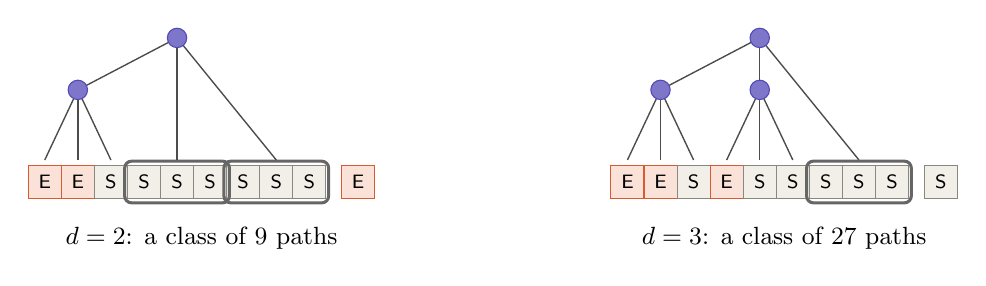
\begin{tikzpicture}
% fig_exA_other.tex, generated by gen_figs.py of the guest session (Claude Fable 5.2 in the Claude app), 2026-11-14; inlined.
\node[ebox] at (1.810,0.210) {\textsf{E}};
\node[ebox] at (2.230,0.210) {\textsf{E}};
\node[sbox] at (2.650,0.210) {\textsf{S}};
\node[sbox] at (3.070,0.210) {\textsf{S}};
\node[sbox] at (3.490,0.210) {\textsf{S}};
\node[sbox] at (3.910,0.210) {\textsf{S}};
\node[sbox] at (4.330,0.210) {\textsf{S}};
\node[sbox] at (4.750,0.210) {\textsf{S}};
\node[sbox] at (5.170,0.210) {\textsf{S}};
\node[ebox] at (5.790,0.210) {\textsf{E}};
\draw[edge] (3.490,2.040) -- (2.230,1.380);
\draw[edge] (2.230,1.380) -- (1.810,0.490);
\draw[edge] (2.230,1.380) -- (2.230,0.490);
\draw[edge] (2.230,1.380) -- (2.650,0.490);
\node[asymn] at (2.230,1.380) {};
\draw[satom] (2.825,-0.055) rectangle (4.155,0.475);
\draw[edge] (3.490,2.040) -- (3.490,0.490);
\draw[satom] (4.085,-0.055) rectangle (5.415,0.475);
\draw[edge] (3.490,2.040) -- (4.750,0.490);
\node[asymn] at (3.490,2.040) {};
\node[font=\small] at (3.80,-0.5) {$d=2$: a class of $9$ paths};
\node[ebox] at (9.210,0.210) {\textsf{E}};
\node[ebox] at (9.630,0.210) {\textsf{E}};
\node[sbox] at (10.050,0.210) {\textsf{S}};
\node[ebox] at (10.470,0.210) {\textsf{E}};
\node[sbox] at (10.890,0.210) {\textsf{S}};
\node[sbox] at (11.310,0.210) {\textsf{S}};
\node[sbox] at (11.730,0.210) {\textsf{S}};
\node[sbox] at (12.150,0.210) {\textsf{S}};
\node[sbox] at (12.570,0.210) {\textsf{S}};
\node[sbox] at (13.190,0.210) {\textsf{S}};
\draw[edge] (10.890,2.040) -- (9.630,1.380);
\draw[edge] (9.630,1.380) -- (9.210,0.490);
\draw[edge] (9.630,1.380) -- (9.630,0.490);
\draw[edge] (9.630,1.380) -- (10.050,0.490);
\node[asymn] at (9.630,1.380) {};
\draw[edge] (10.890,2.040) -- (10.890,1.380);
\draw[edge] (10.890,1.380) -- (10.470,0.490);
\draw[edge] (10.890,1.380) -- (10.890,0.490);
\draw[edge] (10.890,1.380) -- (11.310,0.490);
\node[asymn] at (10.890,1.380) {};
\draw[satom] (11.485,-0.055) rectangle (12.815,0.475);
\draw[edge] (10.890,2.040) -- (12.150,0.490);
\node[asymn] at (10.890,2.040) {};
\node[font=\small] at (11.20,-0.5) {$d=3$: a class of $27$ paths};
\end{tikzpicture}
\caption{Example~\ref{path:ex:A}. Top: the minimal class, as words and as paths from $(0,7)$ to $(3,0)$. The
$9$-segment is the only mixed segment; its three thirds are atoms. Bottom: paths in two of the larger classes. They are not
minimal because their steps $\E$ are split into three atoms of length $1$, while $n=3=(10)_3$ has digit sum $1$.
% Words added 2026-11-15 after the AI review of brief W053, read off the source of the picture; not in the text that was approved.
\revnote{in words, the minimal class consists of $\E\E\E\,\Ss\Ss\Ss\,\Ss\Ss\Ss\,\Ss$,
$\Ss\Ss\Ss\,\E\E\E\,\Ss\Ss\Ss\,\Ss$ and $\Ss\Ss\Ss\,\Ss\Ss\Ss\,\E\E\E\,\Ss$; the two paths of the bottom row are
$\E\E\Ss\,\Ss\Ss\Ss\,\Ss\Ss\Ss\,\E$, marked $d=2$, in a class of $9$ paths, and
$\E\E\Ss\,\E\Ss\Ss\,\Ss\Ss\Ss\,\Ss$, marked $d=3$, in a class of $27$ paths.}}
\label{path:fig:exA}
\end{figure}

\begin{example}[$p=3$, $q=9$, $n=2$]\label{path:ex:B}
Here $m=17=(122)_3$, $N=19=(201)_3$, $C=\frac1{17}\binom{18}2=9$ and $t=(5-1)/2=2$. The top segments are two
segments of length $9$ and one single step. Adding $n=(2)_3$ and $m=(122)_3$ carries into digits $1$ and $2$.
So a minimal path has one mixed segment of length $9$ and one mixed segment of length $3$ inside it
(Figure~\ref{path:fig:exB}). The count of Proposition~\ref{path:prop:count}:

\begin{center}\small
\begin{tabular}{@{}clll@{}}
\toprule
length & slots & to place & ways\\
\midrule
$9$ & the $2$ top segments of length $9$ & one $\Ss$-atom, one mixed & $2!=2$\\
$3$ & the $3$ thirds of the mixed $9$-segment & two $\Ss$-atoms, one mixed & $3!/2!=3$\\
$1$ & the $3$ steps of the mixed $3$-segment, the single step & two $\E$, two $\Ss$ & $4!/(2!\,2!)=6$\\
\bottomrule
\end{tabular}
\end{center}

So there are $2\cdot3\cdot6=36$ minimal paths, in $M=36/3^2=4$ classes. All $\binom{19}2=171$ paths: four classes
of $9$, two of $27$, one of $81$. So $19\cdot C=171=9\cdot4+27\cdot5$, hence $C=9$ and
$C/9=1\equiv4\equiv(-1)^2/(2!\,2!\,1!)\pmod3$.
\end{example}

\begin{figure}[ht]
\centering
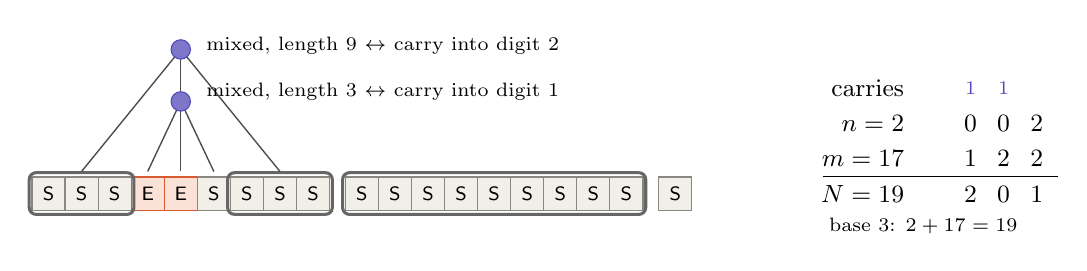
\begin{tikzpicture}
% fig_exB.tex, generated by gen_figs.py of the guest session (Claude Fable 5.2 in the Claude app), 2026-11-14; inlined.
\node[sbox] at (0.210,0.210) {\textsf{S}};
\node[sbox] at (0.630,0.210) {\textsf{S}};
\node[sbox] at (1.050,0.210) {\textsf{S}};
\node[ebox] at (1.470,0.210) {\textsf{E}};
\node[ebox] at (1.890,0.210) {\textsf{E}};
\node[sbox] at (2.310,0.210) {\textsf{S}};
\node[sbox] at (2.730,0.210) {\textsf{S}};
\node[sbox] at (3.150,0.210) {\textsf{S}};
\node[sbox] at (3.570,0.210) {\textsf{S}};
\node[sbox] at (4.190,0.210) {\textsf{S}};
\node[sbox] at (4.610,0.210) {\textsf{S}};
\node[sbox] at (5.030,0.210) {\textsf{S}};
\node[sbox] at (5.450,0.210) {\textsf{S}};
\node[sbox] at (5.870,0.210) {\textsf{S}};
\node[sbox] at (6.290,0.210) {\textsf{S}};
\node[sbox] at (6.710,0.210) {\textsf{S}};
\node[sbox] at (7.130,0.210) {\textsf{S}};
\node[sbox] at (7.550,0.210) {\textsf{S}};
\node[sbox] at (8.170,0.210) {\textsf{S}};
\draw[satom] (-0.035,-0.055) rectangle (1.295,0.475);
\draw[edge] (1.890,2.040) -- (0.630,0.490);
\draw[edge] (1.890,2.040) -- (1.890,1.380);
\draw[edge] (1.890,1.380) -- (1.470,0.490);
\draw[edge] (1.890,1.380) -- (1.890,0.490);
\draw[edge] (1.890,1.380) -- (2.310,0.490);
\node[asymn] at (1.890,1.380) {};
\draw[satom] (2.485,-0.055) rectangle (3.815,0.475);
\draw[edge] (1.890,2.040) -- (3.150,0.490);
\node[asymn] at (1.890,2.040) {};
\draw[satom] (3.945,-0.055) rectangle (7.795,0.475);
\node[font=\scriptsize,anchor=west] at (2.09,2.09) {mixed, length $9$ $\leftrightarrow$ carry into digit $2$};
\node[font=\scriptsize,anchor=west] at (2.09,1.50) {mixed, length $3$ $\leftrightarrow$ carry into digit $1$};
\node[font=\small,anchor=east] at (11.20,1.55) {carries};
\node[font=\small] at (11.92,1.55) {\color{purpline}\scriptsize $1$};
\node[font=\small] at (12.34,1.55) {\color{purpline}\scriptsize $1$};
\node[font=\small,anchor=east] at (11.20,1.10) {$n=2$};
\node[font=\small] at (11.92,1.10) {\small $0$};
\node[font=\small] at (12.34,1.10) {\small $0$};
\node[font=\small] at (12.76,1.10) {\small $2$};
\node[font=\small,anchor=east] at (11.20,0.65) {$m=17$};
\node[font=\small] at (11.92,0.65) {\small $1$};
\node[font=\small] at (12.34,0.65) {\small $2$};
\node[font=\small] at (12.76,0.65) {\small $2$};
\node[font=\small,anchor=east] at (11.20,0.20) {$N=19$};
\node[font=\small] at (11.92,0.20) {\small $2$};
\node[font=\small] at (12.34,0.20) {\small $0$};
\node[font=\small] at (12.76,0.20) {\small $1$};
\draw[line width=0.5pt] (10.05,0.43) -- (13.03,0.43);
\node[font=\scriptsize,anchor=west] at (10.00,-0.20) {base $3$: $2+17=19$};
\end{tikzpicture}
\caption{Example~\ref{path:ex:B}: a minimal path with its two mixed segments, one for each carry of the addition on
the right. Its atoms are two $\E$-atoms of length $1$ and $\Ss$-atoms of lengths $9,3,3,1,1$: the digits of $n=(2)_3$ and
$m=(122)_3$.
% Words added 2026-11-15 after the AI review of brief W053, read off the source of the picture; not in the text that was approved.
\revnote{in words, the pictured path is $\Ss\Ss\Ss\,\E\E\Ss\,\Ss\Ss\Ss$ on the first top segment of length
$9$, nine steps $\Ss$ on the second, and $\Ss$ on the single step; the mixed segment of length $3$ is the
middle third $\E\E\Ss$ of the first top segment. The addition drawn on the right is $2+17=19$ in base $3$,
that is $(002)_3+(122)_3=(201)_3$, with a carry into digit $1$ and a carry into digit $2$.}}
\label{path:fig:exB}
\end{figure}

\subsection{Remarks}\label{path:sec:remarks}

\begin{enumerate}[leftmargin=*,itemsep=4pt]
\item \textbf{What the symmetry acts on.} The moves act on all $N\cdot C$ paths in $\W$. They do not act on the $C$
classes of cyclic shifts, and they do not keep a path under the line of Remark~\ref{path:rem:dyck}: a move and a cyclic
shift do not commute. The passage from $\binom Nn$ to $C$ uses the free cyclic symmetry (Lemma~\ref{path:lem:shift}) and
one arithmetic fact, $N\equiv1\pmod p$.

\item \textbf{It is a statement about binomial coefficients.} Sections \ref{path:sec:moves}--\ref{path:sec:count} never use
$N=qn+1$. Theorem~\ref{path:thm:binom} is classical. According to the introduction of \cite{Granville}, the exponent is Kummer's theorem
(1852), and the congruence was found by Anton (1869), Stickelberger (1890) and Hensel (1902). Theorem~\ref{path:thm:main} is
its special case $\binom{qn+1}n$. What the argument here adds is a proof by a group action, with the carries
visible as mixed segments. We have not searched the literature properly for this proof. The group-action proof of
Lucas' theorem on the Wikipedia page ``Lucas's theorem'' uses only cyclic rotations of blocks of length $p^i$, not nested ones.
Before any claim of novelty this needs a real search. \assembler{a search was made after this note was written, and its two closest sources were read; see
Section~\ref{sec:attribution}. The group, its action on subsets and the recursion for the sizes of the orbits
are in a paper of J.~H.~Smith \cite{Smith}; the count of the smallest orbits with Wilson's theorem is
sketched, for one carry pattern, in an answer of M.~Wildon \cite{Wildon}.}

\item \textbf{Is it a proof ``from symmetries of trees''?} The group is the rotation group of a forest of
complete $p$-ary trees, a Sylow $p$-subgroup of the symmetric group of the steps. In the tree proof such a group
appears as the symmetry group of a minimal tree (the team's note \texttt{notes/2026-11-14\_connections\_ranked.md},
section 3.2); here it acts from the start. But these are the trees of segments, not the $q$-ary trees that $C$ counts
and on which the group of \cite{Konvalinka} acts. Whether this answers Problem~137 is for the team to judge.
% Note added 2026-11-15 after the AI review of brief W053; not in the text that was approved.
\revnote{the answer of this report is in Section~\ref{sec:further}: the lattice-path proof is offered as a
companion to the main proof, not as a proof from the symmetries of the trees.}

\item \textbf{Comparison with the tree proof.}\nopagebreak[4]

\nopagebreak[4]\smallskip
{\small
\begin{tabular}{@{}p{0.17\textwidth}p{0.37\textwidth}p{0.37\textwidth}@{}}
\toprule
 & tree proof & path proof\\
\midrule
objects & $k$-blocked $p$-ary trees, $C$ of them & paths, $N\cdot C$ of them\\
symmetry & rotate the children of any node of the tree & rotate the sub-segments of any segment; the segments are fixed\\
class size & $p^{d}$, $d$ = number of asymmetric nodes & $p^{d}$, $d$ = number of asymmetric segments\\
lower bound & $d\ge t$, digit sums of leaf numbers & $d\ge t$, digit sums of step numbers\\
minimal objects & $m_j$ complete subtrees of height $j$ on a skeleton with $t$ asymmetric nodes
 & $m_j$ $\Ss$-atoms and $n_j$ $\E$-atoms of length $p^j$ under $t$ mixed segments\\
% Clarification added 2026-11-15 after the referee report (report/reviews/REFEREE.md, finding 16); not in the text that was approved.
minimal classes & $|\mathcal S(m,k)|$, evaluated modulo $p$ by the cherry collapse \refnote{$|\mathcal S(m,k)|$ is the number called $N_{\min}$ in Section~\ref{sec:mainproof}} & an explicit product; Wilson's theorem once for each carry\\
\bottomrule
\end{tabular}}

\smallskip
The last row is the difference. On paths the skeleton is rigid: one mixed segment for each carry, so the minimal
classes can be counted level by level. On trees the shape of the skeleton varies, and the cherry collapse does
the count.

\item \textbf{What was checked by computer.} By brute force over all paths: Lemma~\ref{path:lem:size} (also by computing the
classes directly from the moves), Proposition~\ref{path:prop:bound}, Lemma~\ref{path:lem:mixed}, the exact count \eqref{path:eq:M}
and Theorem~\ref{path:thm:binom}, for all $0\le n\le N\le16$ and $p=2,3,5$ ($456$ cases)
% Clarification added 2026-11-15 after the referee report (report/reviews/REFEREE.md, finding 24); not in the text that was approved.
\refnote{the program starts at $N=1$: the $456$ cases are those with $1\le N\le16$}; and Theorem~\ref{path:thm:main} for $34$
pairs $(q,n)$ with $q\in\{2,3,4,5,7,8,9\}$ and $N\le28$. Also Lemma~\ref{path:lem:shift} and
Remark~\ref{path:rem:dyck} for small $(q,n)$. Scripts and their output: \texttt{experiments/path\_segments/} in the folder of that guest session in the repository.
\end{enumerate}

\section{The Frobenius proof (full text)}\label{app:frob}
\noindent\emph{Provenance and status} (this paragraph replaces the box at the head of the stand-alone note; its
second half is the content of that box, its first half was written in assembling the report from the
project's ledger, claim C18). The note below was written on 14 November 2026 by an AI system (Claude
Fable~5.2). \textbf{No human has checked it} (a team member began to read it and stopped for the time being).
A second AI reader (the same model as the author), who saw only
the note, refereed it and found no false statement and no invalid step; the omitted justifications it listed
are filled in this version, and those repairs were not re-reviewed. Every lemma was checked by computer
(experiment E010). The whole chain of lemmas is formalized in Lean (Section~\ref{sec:lean}), with three
differences of method listed there. The text is reproduced unchanged, apart from labels, headings and
cross-references, one marked note on notation added on 15 November after an AI referee's reading of this
report, and one marked note in the remark on earlier algebraic work, added the same day after a second AI
review.

\smallskip\noindent
This appendix proves the theorem of Section~\ref{sec:mainproof} a second time, by algebra only. It is
\emph{self-contained}: it uses no result of Section~\ref{sec:mainproof}, no closed formula for the
Fuss--Catalan numbers, and neither Legendre's nor Kummer's formula for the power of $p$ in a factorial or a
binomial coefficient. The inputs are the equation $G=x+G^q$, Fermat's and Wilson's congruences, the behaviour
of digit sums under addition, and standard algebra (the multinomial theorem, Leibniz' rule, uniqueness of
base-$p$ expansions). The only divisibility facts about factorials are the trivial ones: $p\nmid n!$ for
$n<p$, $p\mid\binom{pb}{b}$, and $p\mid p!/(n_1!\cdots n_p!)$ when all $n_i<p$. The two proofs share no
lemma, so each is a check on the other. Section~\ref{frob:sec:dict} explains that every step here is the
generating function of one step of the tree proof. Being algebra, it is not a proof ``from symmetries of
trees''; it is offered as a check on the main proof and an explanation of it.


% ---- Source: paper/frobenius_proof.tex. Provenance lines of the source file:
% Written by Claude Fable 5.2 (AI, orchestrator), 2026-11-14. A third proof, purely algebraic ("Frobenius").
% Every lemma is checked numerically in experiments/E010_frobenius_complete/run.py. Not human-verified.
% It replaces the incomplete worker draft alt_proof_frobenius.tex (Kimi K3.1 Pro, four marked gaps).
% ---- Merged mechanically by Claude Fable 5.2 (worker W046), 2026-11-15: labels prefixed with frob:,
% ---- sections demoted one level, title, status box and bibliography removed, two references to
% ---- sections repaired. The mathematical text is unchanged.
% ---- Claude Fable 5.2 (referee, brief W052), 2026-11-15: one note added in the remark on delta-rings
% ---- (macro \refnote, preceded by a comment line).
% ---- Claude Fable 5.2 (reviewer, brief W053), 2026-11-15: one note added at the end of the remark "Earlier
% ---- algebraic work" (macro \revnote, preceded by a comment line). Nothing else in this appendix was changed.
\subsection{Statement}\label{frob:sec:statement}

Let $p$ be a prime, $k\ge1$ and $q=p^k$. Let $G(x)\in\Z[[x]]$ be the unique power series
without constant term such that
\begin{equation}\label{frob:eq:G}
 G=x+G^{q}.
\end{equation}
(The coefficient of $x^m$ on the right involves only coefficients of $G$ of lower degree, so
$G$ exists and is unique.) \textbf{Throughout this note, $\C$ denotes the coefficient of
$x^{(q-1)n+1}$ in $G$.} This is the number of $q$-ary trees with $n$ internal nodes: such a
tree is a leaf or a root with $q$ subtrees, so if $x$ marks the leaves the generating
function of $q$-ary trees satisfies \eqref{frob:eq:G}, and a tree with $n$ internal nodes has
$(q-1)n+1$ leaves. That sentence is the only place where a tree is used, and only to say what
the theorem is about. The closed formula $\C=\binom{qn}{n}/((q-1)n+1)$ is classical (Lagrange
inversion); it is not used.

Notation: $\N=\{0,1,2,\dots\}$. For an integer $m\ge0$ write $m=\sum_{j\ge0}m_jp^j$ in base
$p$ and $s_p(m)=\sum_jm_j$ (so $s_p(0)=0$).

\begin{theorem}\label{frob:thm}
Let $n\ge0$, $m=(q-1)n+1$ and $t=(s_p(m)-1)/(p-1)$. Then $t$ is a non-negative integer and
\[
 \C\cdot\prod_{j}m_j!\;\equiv\;(-p)^{t}\pmod{p^{\,t+1}} .
\]
In particular $v_p(\C)=t$ and $\C/p^{t}\equiv(-1)^t/\prod_jm_j!\pmod p$.
\end{theorem}

($t$ is an integer because $s_p(m)\equiv m\equiv1\pmod{p-1}$. Each $m_j!$ is prime to $p$.)

\subsection{Three elementary facts}

\begin{enumerate}[label=\textbf{(E\arabic*)},leftmargin=3.2em]
\item\label{frob:E1} \emph{Digit sums.} Let $n_1,\dots,n_r\ge0$ be integers. Call the sum
$n_1+\dots+n_r$ \emph{carry-free} if for every $j$ the $j$-th base-$p$ digits of the $n_i$
add up to at most $p-1$. Then
\[
 s_p(n_1+\dots+n_r)\le s_p(n_1)+\dots+s_p(n_r),\quad\text{with equality exactly when the sum
 is carry-free.}
\]
\emph{Proof.} Let $D_j$ be the sum of the $j$-th digits, so $\sum_in_i=\sum_jD_jp^j$ and
$\sum_jD_j=\sum_is_p(n_i)$. While some $D_j\ge p$, replace $(D_j,D_{j+1})$ by
$(D_j-p,\,D_{j+1}+1)$: the number represented is unchanged and $\sum_jD_j$ drops by $p-1\ge1$.
This stops, and it stops at the base-$p$ expansion of $\sum_in_i$. So
$s_p(\sum_in_i)=\sum_is_p(n_i)-(p-1)\cdot(\text{number of steps})$, and no step is made
exactly when the sum is carry-free. \qed

Two further facts. First, $s_p(pn)=s_p(n)$, because multiplying by $p$ shifts the digits one
place. Second, a sum of $p$ equal numbers $n+\dots+n$ $(n\ge1)$ is never carry-free, because a
non-zero digit $e$ of $n$ gives $D_j=pe\ge p$.

\item\label{frob:E2} \emph{Cyclic shifts.} The cyclic group of order $p$ acts on $p$-tuples
(of anything) by cyclic shift. As $p$ is prime, a tuple fixed by a non-trivial shift is
constant. So the non-constant $p$-tuples fall into orbits of exactly $p$ tuples.

\item\label{frob:E3} \emph{Fermat and Wilson.} $c^p\equiv c\pmod p$ for every integer $c$, and
$(p-1)!\equiv-1\pmod p$.
\end{enumerate}

\subsection{The Frobenius lift and a deformation of the equation}

Let $\Lambda=\Z[y][[x]]$: power series in $x$ whose coefficients are polynomials in $y$. Its
\emph{monomials} are the $x^my^d$. Let $\varphi\colon\Lambda\to\Lambda$ be the ring
endomorphism $\varphi(f)(x,y)=f(x^p,y^p)$; on a monomial, $\varphi(\mu)=\mu^p$.

\begin{lemma}\label{frob:lem:theta}
Let $f=\sum_ic_i\mu_i\in\Lambda$, with distinct monomials $\mu_i$ and integers $c_i$. Then
\begin{equation}\label{frob:eq:theta}
 \theta(f):=\frac{f^p-\varphi(f)}{p}
 =\frac1p\sum_{\substack{(i_1,\dots,i_p)\\ \text{not constant}}}
   c_{i_1}\cdots c_{i_p}\,\mu_{i_1}\cdots\mu_{i_p}
  \;+\;\sum_i\frac{c_i^{\,p}-c_i}{p}\,\mu_i^{\,p}
\end{equation}
has integer coefficients, that is, $\theta(f)\in\Lambda$. In particular every monomial that
occurs in $\theta(f)$ is a product of $p$ monomials that occur in $f$.
\end{lemma}

\begin{proof}
Expand $f^p$ as a sum over $p$-tuples of indices. The series $f$ may have infinitely many
monomials, but only finitely many of each $x$-degree (its coefficients are polynomials in
$y$), and $x$-degrees are non-negative; so a given monomial of $f^p$ is produced by finitely
many tuples. The constant tuples give $\sum_ic_i^p\mu_i^p$, and
$\varphi(f)=\sum_ic_i\mu_i^p$; this gives the formula. For a fixed monomial, the set of
non-constant tuples producing it is finite and stable under cyclic shifts, and the tuples of
an orbit contribute equal terms; so the first sum is divisible by $p$ by \ref{frob:E2}. The second
is divisible by $p$ by Fermat.
\end{proof}

So $f^p=\varphi(f)+p\,\theta(f)$: raising to the $p$-th power is the Frobenius substitution
plus $p$ times a correction. We now replace that factor $p$ by the variable $y$.

\begin{lemma}\label{frob:lem:system}
There are unique series $F_\delta\in\Lambda$, $\delta\in\Z/k$, without terms of $x$-degree
$0$, such that
\begin{equation}\label{frob:eq:system}
 F_\delta=\br{\delta=0}\,x+\varphi(F_{\delta+1})+y\,\theta(F_{\delta+1})
 \qquad(\delta\in\Z/k),
\end{equation}
where $\br{\cdot}$ is $1$ if the condition holds and $0$ otherwise. Moreover
$F_0(x,p)=G(x)$.
\end{lemma}

\begin{proof}
We define the coefficients of $x^m$ of all the $F_\delta$ together, by recursion on $m\ge1$.
Suppose the coefficients of $x$-degree less than $m$ are known, lie in $\Z[y]$, and that there
is none of degree $0$; let $P_\delta\in\Z[y][x]$ be the resulting polynomial truncation of
$F_\delta$. For any series $f$ without terms of $x$-degree $0$, the coefficient of $x^m$ in
$\varphi(f)$ is determined by the coefficient of $x^{m/p}$ in $f$, and the coefficient of
$x^m$ in $f^p$ by the coefficients of $f$ of $x$-degree at most $m-p+1$, because a product of
$p$ monomials of positive $x$-degree is involved. As $m/p<m$ and $m-p+1<m$, the coefficient
of $x^m$ on the right of \eqref{frob:eq:system} must be the coefficient of $x^m$ in
$\br{\delta=0}x+\varphi(P_{\delta+1})+y\,\theta(P_{\delta+1})$, and this is a polynomial in
$y$ with integer coefficients by Lemma~\ref{frob:lem:theta}, applied to the polynomial
$P_{\delta+1}$. It has no term of degree $0$. This proves existence and uniqueness.

Setting $y=p$ is a ring homomorphism $\varepsilon\colon\Lambda\to\Z[[x]]$, and
$\varepsilon(\varphi(f)+y\theta(f))=\varepsilon(\varphi(f)+p\theta(f))=\varepsilon(f^p)
=\varepsilon(f)^p$. Hence $g_\delta=\varepsilon(F_\delta)$ satisfy
$g_\delta=\br{\delta=0}x+g_{\delta+1}^{\,p}$, that is,
$g_0=x+g_1^p$, $g_1=g_2^p$, \dots, $g_{k-1}=g_0^p$. So $g_0=x+g_0^{p^k}$, and $g_0=G$ by
uniqueness in \eqref{frob:eq:G}.
\end{proof}

For $k=1$ the system is the single equation $F=x+\varphi(F)+y\,\theta(F)$.

\subsection{Weights: the lower bound}

\begin{definition}
The \emph{weight} of a monomial $x^my^d$ with $m\ge1$ is $w(x^my^d)=(p-1)d-s_p(m)$.
\end{definition}

By \ref{frob:E1}, for monomials $\mu_1,\dots,\mu_r$ of positive $x$-degree,
\begin{equation}\label{frob:eq:wprod}
 w(\mu_1\cdots\mu_r)\ge w(\mu_1)+\dots+w(\mu_r),\quad\text{with equality exactly when the
 $x$-exponents add carry-free,}
\end{equation}
and, since $\varphi(x^my^d)=x^{pm}y^{pd}$ and $s_p(pm)=s_p(m)$,
\begin{equation}\label{frob:eq:wphi}
 w(\varphi(\mu))=w(\mu)+(p-1)^2d\;\ge\;w(\mu),\quad\text{with equality exactly when }d=0.
\end{equation}

\begin{lemma}[Lower bound]\label{frob:lem:lower}
Every monomial occurring in any $F_\delta$ has weight at least $-1$.
\end{lemma}

\begin{proof}
Induction on the $x$-degree $m$. By \eqref{frob:eq:system} and Lemma~\ref{frob:lem:theta}, a monomial of
$F_\delta$ of $x$-degree $m$ is $x$ (weight $-1$), or $\varphi(\mu)$, or $y\mu_1\cdots\mu_p$,
where $\mu,\mu_1,\dots,\mu_p$ are monomials of $F_{\delta+1}$ of $x$-degree less than $m$. By
induction these have weight $\ge-1$, so $w(\varphi(\mu))\ge-1$ by \eqref{frob:eq:wphi} and
$w(y\mu_1\cdots\mu_p)\ge(p-1)-p=-1$ by \eqref{frob:eq:wprod}.
\end{proof}

\begin{corollary}\label{frob:cor:div}
For $m=(q-1)n+1$, the polynomial $[x^m]F_0\in\Z[y]$ is divisible by $y^t$. Hence $p^t$
divides $\C=[x^m]F_0(x,p)$.
\end{corollary}

\subsection{The leading part: a carry-free product}

For $\delta\in\Z/k$ and $m\ge1$ with $s_p(m)\equiv1\pmod{p-1}$ let $\ell_\delta(m)\in\Z$ be
the coefficient of $x^my^{(s_p(m)-1)/(p-1)}$ in $F_\delta$; for all other $m\ge0$ put
$\ell_\delta(m)=0$. These are the coefficients of the monomials of weight exactly $-1$.

\begin{definition}
Let $\A$ be the set of functions $f\colon\Z_{\ge0}\to\Q$ with the \emph{carry-free product}
\[
 (f\cf g)(m)=\sum_{\substack{n_1+n_2=m,\ n_1,n_2\ge0\\ n_1+n_2\text{ carry-free}}}f(n_1)\,g(n_2).
\]
\end{definition}

$\A$ is a commutative, associative $\Q$-algebra whose unit is the indicator function of
$\{0\}$: by the definition in \ref{frob:E1}, $(n_1+n_2)+n_3$ is carry-free with $n_1+n_2$
carry-free exactly when the digits of $n_1,n_2,n_3$ add up to at most $p-1$ in every
position, a symmetric condition. So $f^{\cf r}(m)$ is the sum of $f(n_1)\cdots f(n_r)$ over
the carry-free $r$-tuples $(n_1,\dots,n_r)$ of non-negative integers with sum $m$. The value
of a product at $m$ involves only the values of its factors on $\{0,\dots,m\}$. Let
$\alpha_\delta\in\A$ be the indicator function of $\{p^j:\ j\ge0,\ j\equiv-\delta\pmod k\}$.

\begin{lemma}[Leading part]\label{frob:lem:lead}
\begin{enumerate}[label=(\roman*)]
\item $F_\delta(x,0)=\sum_{j\ge0,\ j\equiv-\delta\ (k)}x^{p^j}$ for every $\delta$.
\item $\displaystyle \ell_\delta=\alpha_\delta+\frac1p\,\ell_{\delta+1}^{\;\cf p}$ in $\A$,
      for every $\delta\in\Z/k$.
\end{enumerate}
\end{lemma}

\begin{proof}
(i) Put $y=0$ in \eqref{frob:eq:system}: the series $f_\delta=F_\delta(x,0)$ satisfy
$f_\delta(x)=\br{\delta=0}x+f_{\delta+1}(x^p)$. The series
$A_\delta=\sum_{j\equiv-\delta}x^{p^j}$ satisfy the same equations, because
$A_{\delta+1}(x^p)=\sum_{j\ge1,\ j\equiv-\delta}x^{p^{j}}$ and the missing term $x=x^{p^0}$
belongs to $A_\delta$ exactly when $\delta=0$. Among series without constant term the solution
is unique (recursion on the degree), and neither $f_\delta$ nor $A_\delta$ has a constant term.

(ii) Collect the monomials of weight $-1$ on both sides of \eqref{frob:eq:system}.

\emph{The terms $\br{\delta=0}x$ and $\varphi(F_{\delta+1})$.} By \eqref{frob:eq:wphi} and
Lemma~\ref{frob:lem:lower}, $\varphi(\mu)$ has weight $-1$ only if $\mu$ has weight $-1$ and
contains no $y$. By (i) such $\mu$ are the $x^{p^j}$ with $j\equiv-\delta-1$, each with
coefficient $1$. Together with $\br{\delta=0}x$ this gives $A_\delta$, as in (i); its
coefficients are $\alpha_\delta$.

\emph{The term $y\theta(F_{\delta+1})$.} Use \eqref{frob:eq:theta} for $f=F_{\delta+1}$. By
\eqref{frob:eq:wprod} and Lemma~\ref{frob:lem:lower}, $y\mu_{i_1}\cdots\mu_{i_p}$ has weight
$\ge(p-1)-p=-1$, with equality exactly when every $\mu_{i_j}$ has weight $-1$ and their
$x$-exponents add carry-free. A constant tuple is never carry-free \ref{frob:E1}. So the second sum
in \eqref{frob:eq:theta} contributes nothing in weight $-1$, and the first contributes
$\frac1p$ times the sum of $c_{i_1}\cdots c_{i_p}\cdot y\mu_{i_1}\cdots\mu_{i_p}$ over the
carry-free $p$-tuples of monomials of weight $-1$ of $F_{\delta+1}$.

It remains to read off the coefficients. A monomial of weight $-1$ is determined by its
$x$-exponent: it is $x^ny^{(s_p(n)-1)/(p-1)}$, it exists only if $s_p(n)\equiv1\pmod{p-1}$,
and its coefficient in $F_{\delta+1}$ is $\ell_{\delta+1}(n)$. So choosing a carry-free
$p$-tuple of monomials of weight $-1$ is the same as choosing a carry-free $p$-tuple
$(n_1,\dots,n_p)$ of positive integers; and since $\ell_{\delta+1}(n)=0$ when $n=0$ or when
$F_{\delta+1}$ has no monomial of weight $-1$ with $x$-exponent $n$, we may sum over all
carry-free $p$-tuples of non-negative integers. For such a tuple with sum $m$, the monomial
$y\mu_{i_1}\cdots\mu_{i_p}$ has $x$-exponent $m$ and weight $-1$, so it is the monomial
$x^my^{(s_p(m)-1)/(p-1)}$ whose coefficient defines $\ell_\delta(m)$; the exponents of $y$
take care of themselves. Hence the weight $-1$ part of $y\theta(F_{\delta+1})$ has
coefficient $\frac1p\,\ell_{\delta+1}^{\;\cf p}(m)$ at $x$-exponent $m$, for every $m$ with
$s_p(m)\equiv1\pmod{p-1}$.

For the remaining $m$ (namely $m=0$, or $s_p(m)\not\equiv1$) both sides of (ii) vanish:
$\ell_\delta(m)=0$ by definition, $\alpha_\delta(m)=0$, and
$\ell_{\delta+1}^{\;\cf p}(m)=0$ because a carry-free sum of $p$ integers $n_i$ with
$s_p(n_i)\equiv1$ has digit sum $\equiv p\equiv1\pmod{p-1}$ and is positive.
\end{proof}

\subsection{The labelled series and the carry operator}

Let $z=(z_c)_{c\in\Z/k}$ be $k$ variables. For $a\in\N^k$ (indexed by $\Z/k$) write
$z^a=\prod_cz_c^{a_c}$, $a!=\prod_ca_c!$, $|a|=\sum_ca_c$, and let $e_c$ be the unit vectors.

\begin{lemma}\label{frob:lem:H}
There are unique $H_\delta\in\Q[[z]]$, $\delta\in\Z/k$, without constant term, such that
\begin{equation}\label{frob:eq:H}
 H_\delta=z_{-\delta}+\frac1p\,H_{\delta+1}^{\,p}\qquad(\delta\in\Z/k).
\end{equation}
Write $H_\delta=\sum_{a\ne0}T_\delta(a)\,z^a/a!$ with $T_\delta(a)\in\Q$.
\end{lemma}

\begin{proof}
The part of degree $n$ of $H_{\delta+1}^p$ involves the parts of $H_{\delta+1}$ of degree at
most $n-p+1<n$. Recursion on $n$.
\end{proof}

\begin{lemma}[From the leading part to the labelled series]\label{frob:lem:subst}
For every $\delta$ and every $m\ge1$ with digits $m_j$,
\[
 \ell_\delta(m)\cdot\prod_jm_j!\;=\;T_\delta\bigl(a(m)\bigr),\qquad
 a(m)_c=\sum_{j\equiv c\ (k)}m_j .
\]
\end{lemma}

\begin{proof}
Let $u_c\in\A$ be the indicator function of $\{p^j:\ j\equiv c\pmod k\}$, so that
$\alpha_\delta=u_{-\delta}$. Each $u_c$ vanishes at $0$, so $u^{\cf a}=\prod_cu_c^{\cf a_c}$
vanishes at every $m<|a|$, and for $P=\sum_aP_az^a\in\Q[[z]]$ the value
$P(u)(m)=\sum_aP_a\,u^{\cf a}(m)$ is a finite sum. The map $P\mapsto P(u)$ is a ring
homomorphism $\Q[[z]]\to\A$: it is clearly additive, and $(PQ)(u)(m)$ and
$(P(u)\cf Q(u))(m)$ are the same finite sum of the terms
$P_aQ_{a'}\,u^{\cf(a+a')}(m)$, because $u^{\cf a}\cf u^{\cf a'}=u^{\cf(a+a')}$ in the
commutative, associative algebra $\A$. Applied to \eqref{frob:eq:H} it shows that
$h_\delta=H_\delta(u)$ satisfy $h_\delta=\alpha_\delta+\frac1p h_{\delta+1}^{\cf p}$ and
$h_\delta(0)=0$. The functions $\ell_\delta$ satisfy the same equations
(Lemma~\ref{frob:lem:lead}(ii)) and also vanish at $0$, by definition. For functions vanishing at
$0$ these equations determine the value at $m\ge1$ from the values at smaller arguments: a
$p$-tuple containing a zero contributes nothing, and the entries of a $p$-tuple of positive
integers with sum $m$ are smaller than $m$. Hence $\ell_\delta=H_\delta(u)$. (Vanishing at
$0$ is needed here: the tuple $(m,0,\dots,0)$ is carry-free.)

It remains to evaluate $u^{\cf a}/a!$ at $m$. Let $\xi_j\in\A$ be the indicator function of
$\{p^j\}$. A sum of $\beta$ copies of $p^j$ is carry-free exactly when $\beta\le p-1$, so
$\xi_j^{\cf\beta}$ is the indicator function of $\{\beta p^j\}$ for $\beta\le p-1$ and is $0$
for $\beta\ge p$; and for $\beta_j\le p-1$ the product of the $\xi_j^{\cf\beta_j}$ over $j$
is the indicator function of $\{\sum_j\beta_jp^j\}$. Now $u_c$ agrees on $\{0,\dots,m\}$
with the \emph{finite} sum of the $\xi_j$ over $j\equiv c$, $p^j\le m$, and the value of a
product at $m$ involves only the values of the factors on $\{0,\dots,m\}$. So we may apply
the multinomial theorem to these finite sums:
\[
 \frac{u^{\cf a}}{a!}(m)=\sum_{(\beta_j)}\ \prod_j\frac1{\beta_j!},
\]
the sum being over the families $(\beta_j)_{j\ge0}$ of integers with $0\le\beta_j\le p-1$,
$\sum_{j\equiv c}\beta_j=a_c$ for all $c$, and $\sum_j\beta_jp^j=m$. By uniqueness of the
base-$p$ expansion, the only candidate is $\beta_j=m_j$, and it occurs exactly when
$a=a(m)$. Hence $H_\delta(u)(m)=T_\delta(a(m))/\prod_jm_j!$.
\end{proof}

\paragraph{Hurwitz series.} Let $\Hur\subset\Q[[z]]$ be the set of series
$\sum_af_a\,z^a/a!$ with all $f_a\in\Z$, and $\partial_c=\partial/\partial z_c$.

\begin{lemma}\label{frob:lem:hur}
\begin{enumerate}[label=(\roman*)]
\item $\Hur$ is a subring of $\Q[[z]]$, and $\partial_c\Hur\subset\Hur$; indeed
      $\partial_c(z^a/a!)=z^{a-e_c}/(a-e_c)!$ (zero if $a_c=0$).
\item If $f\in\Hur$ has no constant term, then $f^p\in p\,\Hur$.
\item If $g\in\Hur$ has constant term $g_0$, then $g^p\equiv g_0\pmod{p\,\Hur}$.
\item If $f\in\Hur$ has no constant term and $h=f^p/p$, then for every $c$
\[
 \partial_ch=f^{p-1}\,\partial_cf,\qquad
 \partial_c^{\,p}h\equiv f^{p-1}\,\partial_c^{\,p}f-(\partial_cf)^p\pmod{p\,\Hur}.
\]
\end{enumerate}
\end{lemma}

\begin{proof}
(i) $\frac{z^a}{a!}\cdot\frac{z^b}{b!}=\prod_c\binom{a_c+b_c}{a_c}\cdot\frac{z^{a+b}}{(a+b)!}$.

(ii) Write $f=\sum_{a\ne0}f_a\,z^a/a!$ and expand $f^p$ over $p$-tuples $(a^1,\dots,a^p)$ of
non-zero indices; each coefficient of $f^p$ receives finitely many contributions. Each term is
in $\Hur$ by (i), and the non-constant tuples come in orbits of $p$ equal terms \ref{frob:E2}. A
constant tuple contributes $f_a^p\,(z^a/a!)^p=f_a^p\,\frac{(pa)!}{(a!)^p}\cdot\frac{z^{pa}}{(pa)!}$,
and $\frac{(pa)!}{(a!)^p}=\prod_c\frac{(pa_c)!}{(a_c!)^p}$ is a product of multinomial
coefficients. For $b\ge1$,
$\frac{(pb)!}{(b!)^p}=\binom{pb}{b}\cdot\frac{((p-1)b)!}{(b!)^{p-1}}$ and
$\binom{pb}{b}=p\binom{pb-1}{b-1}$, so this integer is divisible by $p$ as $a\ne0$.

(iii) Write $g=g_0+g_+$. In $g^p=\sum_i\binom pig_0^{p-i}g_+^{\,i}$ the terms with $0<i<p$
are in $p\Hur$, $g_+^{\,p}\in p\Hur$ by (ii), and $g_0^p\equiv g_0$ by Fermat.

(iv) The first formula is the chain rule. For the second write $\partial=\partial_c$; by
Leibniz' rule
\[
 \partial^{\,p}(f^p)=\sum_{\substack{(n_1,\dots,n_p)\in\N^p\\ n_1+\dots+n_p=p}}
 \frac{p!}{n_1!\cdots n_p!}\ \prod_{i=1}^p\partial^{\,n_i}f .
\]
The $p$ tuples with one entry equal to $p$ give $p\,f^{p-1}\partial^{\,p}f$. The tuple
$(1,\dots,1)$ gives $p!\,(\partial f)^p$. Every other tuple is non-constant and has all
$n_i\le p-1$: its multinomial coefficient is divisible by $p$, and its orbit under cyclic
shifts consists of $p$ tuples with the same term \ref{frob:E2}. So these tuples contribute an
element of $p^2\Hur$. Dividing by $p$ and using Wilson, $(p-1)!\equiv-1$, gives the claim.
\end{proof}

\begin{proposition}[The carry operator]\label{frob:prop:carry}
All $H_\delta$ lie in $\Hur$, that is, $T_\delta(a)\in\Z$. For all $\delta,c\in\Z/k$,
\[
 \bigl(\partial_c^{\,p}+\partial_{c+1}\bigr)H_\delta\in p\,\Hur ,
 \qquad\text{equivalently}\qquad
 T_\delta(b+p\,e_c)+T_\delta(b+e_{c+1})\equiv0\pmod p\quad\text{for all }b\in\N^k .
\]
\end{proposition}

\begin{proof}
\emph{Integrality.} Let $H_\delta^{\le n}$ be the part of $H_\delta$ of degree at most $n$
(a truncation of an element of $\Hur$ is in $\Hur$). We show by induction on $n$, for all
$\delta$ at once, that $H_\delta^{\le n}\in\Hur$. For $n=1$, $H_\delta^{\le1}=z_{-\delta}$.
If $H_{\delta+1}^{\le n}\in\Hur$, then, as it has no constant term,
$\frac1p(H_{\delta+1}^{\le n})^p\in\Hur$ by Lemma~\ref{frob:lem:hur}(ii); and it agrees with
$\frac1pH_{\delta+1}^p$ in degrees $\le n+1$, because a term of degree at most $n+1$ of a
product of $p$ series without constant term involves only their terms of degree at most
$n+1-(p-1)\le n$. So $H_\delta^{\le n+1}\in\Hur$ by \eqref{frob:eq:H}.

\emph{The congruence.} This part uses the integrality just proved: every $H_\delta$ lies in
$\Hur$ and has no constant term, so Lemma~\ref{frob:lem:hur}(iv) applies to it; and $p\Hur$ is an
ideal of $\Hur$, so a congruence modulo $p\Hur$ may be multiplied by an element of $\Hur$.
Fix $c$ and put $E=\partial_c^{\,p}+\partial_{c+1}$; each $E\,H_\delta$ lies in $\Hur$ by
Lemma~\ref{frob:lem:hur}(i). By \eqref{frob:eq:H},
$H_\delta=z_{-\delta}+h$ with $h=H_{\delta+1}^p/p$. By Lemma~\ref{frob:lem:hur}(iv),
\begin{align*}
 \partial_{c+1}H_\delta&=\br{c+1=-\delta}+H_{\delta+1}^{p-1}\,\partial_{c+1}H_{\delta+1},\\
 \partial_c^{\,p}H_\delta&\equiv H_{\delta+1}^{p-1}\,\partial_c^{\,p}H_{\delta+1}
   -(\partial_cH_{\delta+1})^p\pmod{p\Hur}
\end{align*}
(note $\partial_c^{\,p}z_{-\delta}=0$ as $p\ge2$). By Lemma~\ref{frob:lem:hur}(iii),
$(\partial_cH_{\delta+1})^p$ is congruent to the constant term of $\partial_cH_{\delta+1}$,
which is the coefficient of $z_c$ in $H_{\delta+1}$, namely $\br{c=-\delta-1}$ by
\eqref{frob:eq:H}. The two brackets are the same condition and cancel. Hence
\[
 E\,H_\delta\equiv H_{\delta+1}^{p-1}\cdot E\,H_{\delta+1}\pmod{p\Hur}\qquad
 \text{for all }\delta .
\]
Applying this $k$ times, $E\,H_\delta\equiv\Pi\cdot E\,H_\delta$ with
$\Pi=\prod_{\delta'\in\Z/k}H_{\delta'}^{p-1}\in\Hur$, a series without constant term. So
$E\,H_\delta\equiv\Pi^{\,r}\,E\,H_\delta$ for every $r$, and $\Pi^r$ has no terms of degree
below $r$. Hence every coefficient of $E\,H_\delta$ is divisible by $p$. Finally, by
Lemma~\ref{frob:lem:hur}(i) the coefficient of $z^b/b!$ in $E\,H_\delta$ is
$T_\delta(b+pe_c)+T_\delta(b+e_{c+1})$.
\end{proof}

\begin{proposition}[Evaluation]\label{frob:prop:eval}
Identify $\Z/k$ with $\{0,1,\dots,k-1\}$, so that $p^c$ is defined for $c\in\Z/k$.
Let $a\in\N^k$, $a\ne0$, with $\sum_{c=0}^{k-1}a_cp^c\equiv1\pmod{q-1}$. Then
$|a|\equiv1\pmod{p-1}$ and
\[
 T_0(a)\equiv(-1)^{(|a|-1)/(p-1)}\pmod p .
\]
\end{proposition}

\begin{proof}
$|a|\equiv\sum_ca_cp^c\equiv1\pmod{p-1}$ because $p-1$ divides $q-1$. Induction on $|a|$.

If some $a_c\ge p$, put $a'=a-pe_c+e_{c+1}$ (indices modulo $k$: for $c=k-1$ the index
$c+1$ is $0$). Then $a'\in\N^k$,
$|a'|=|a|-(p-1)\ge1$, and $\sum_ca'_cp^c\equiv\sum_ca_cp^c\pmod{q-1}$, because
$p\cdot p^c=p^{c+1}$ for $c<k-1$ and $p\cdot p^{k-1}=q\equiv1=p^0$. By
Proposition~\ref{frob:prop:carry} with $b=a-pe_c$ and by induction,
$T_0(a)\equiv-T_0(a')\equiv(-1)^{1+(|a'|-1)/(p-1)}=(-1)^{(|a|-1)/(p-1)}$.

If every $a_c\le p-1$, then $1\le\sum_ca_cp^c\le(p-1)(1+p+\dots+p^{k-1})=q-1$, and the only
integer in this range congruent to $1$ modulo $q-1$ is $1$. So $a=e_0$, and $T_0(e_0)=1$ by
\eqref{frob:eq:H}.
\end{proof}

\begin{remark}[Where the hypothesis comes from]\label{frob:rem:support}
Not used in the proof. Give $z_c$ the weight $p^c$, $c\in\{0,\dots,k-1\}$. Then every monomial
$z^a$ of $H_\delta$ has weight $\sum_ca_cp^c\equiv p^{-\delta}\pmod{q-1}$, where $p^{-1}$ is
the inverse of $p$ modulo $q-1$ (it exists because $p^k=q\equiv1$). Indeed, by induction on
the degree in \eqref{frob:eq:H}: $z_{-\delta}$ has weight $1$ if $\delta=0$ and
$p^{k-\delta}\equiv p^{-\delta}$ otherwise, and a product of $p$ monomials of $H_{\delta+1}$
has weight $\equiv p\cdot p^{-\delta-1}=p^{-\delta}$. So $T_0(a)=0$ unless
$\sum_ca_cp^c\equiv1\pmod{q-1}$: the hypothesis of Proposition~\ref{frob:prop:eval} is exactly
the condition under which $T_0(a)$ can be non-zero, and then it is non-zero modulo $p$.
\end{remark}

\subsection{Proof of Theorem~\ref{frob:thm}}

Let $m=(q-1)n+1$ and write $[x^m]F_0=\sum_dc_dy^d$. By Lemma~\ref{frob:lem:system},
$\C=\sum_dc_dp^d$. By Lemma~\ref{frob:lem:lower}, $c_d=0$ unless $(p-1)d\ge s_p(m)-1$, that is,
$d\ge t$; and $c_t=\ell_0(m)$ by definition. Hence
\[
 \C\equiv\ell_0(m)\,p^t\pmod{p^{t+1}} .
\]
By Lemma~\ref{frob:lem:subst}, $\ell_0(m)\prod_jm_j!=T_0(a(m))$. Now $a(m)\ne0$,
$|a(m)|=s_p(m)$, and since $p^j\equiv p^{\,j\bmod k}\pmod{q-1}$,
\[
 \sum_{c=0}^{k-1}a(m)_c\,p^c\equiv\sum_jm_jp^j=m\equiv1\pmod{q-1}.
\]
So Proposition~\ref{frob:prop:eval} gives $T_0(a(m))\equiv(-1)^t\pmod p$, and therefore
$\C\prod_jm_j!\equiv p^t\,T_0(a(m))\equiv(-p)^t\pmod{p^{t+1}}$. \qed

\subsection{What each step means for trees}\label{frob:sec:dict}

None of this section is used above. Read a $q$-ary node as a complete $p$-ary block of height
$k$; then $q$-ary trees are the $p$-ary trees whose leaves all have depth divisible by $k$.
Call two such trees equivalent if one is obtained from the other by cyclically rotating the
$p$ subtrees at some nodes, and call a node \emph{symmetric} if its $p$ subtrees are pairwise
equivalent.

\begin{center}
\begin{tabular}{p{0.44\linewidth}p{0.5\linewidth}}
\textbf{In this note} & \textbf{In the tree proof (Section~\ref{sec:mainproof})}\\\hline
$F_\delta(x,y)$ & classes of trees with root at depth $\delta$; $x$ marks leaves, $y$ marks
                  asymmetric nodes\\
$\varphi(F)$: the Frobenius substitution & a symmetric node: $p$ copies of one class\\
$y\,\theta(F)$: the correction to Frobenius & an asymmetric node: a non-constant cyclic word
                  of $p$ classes\\
$y\mapsto p$ gives $G$ & a class with $d$ asymmetric nodes has $p^d$ trees\\
weight $\ge-1$ (Lemma~\ref{frob:lem:lower}) & $d\ge t$, by digit sums\\
$F_\delta(x,0)=\sum x^{p^j}$ & the complete trees (``atoms'') and their depth condition\\
carry-free product, Lemma~\ref{frob:lem:lead} & minimal classes are skeletons of atoms\\
division by $\prod m_j!$, Lemma~\ref{frob:lem:subst} & equal atoms can be permuted freely\\
$H_\delta$, $T_\delta(a)$ & cyclic trees with distinctly labelled leaves\\
$\partial_c^{\,p}+\partial_{c+1}$ kills $H$ modulo $p$ & a carry is a collapsing cherry\\
Proposition~\ref{frob:prop:eval} & carries until one atom is left\\
\end{tabular}
\end{center}

That the coefficient of $x^my^d$ in $F_0$ is the number of classes with $m$ leaves and $d$
asymmetric nodes was confirmed by listing all classes for small sizes (check ``TREE'' of
experiment E010). The two proofs are logically independent: the tree proof never uses a
generating function, and this note uses trees only to say what $\C$ counts (Section~\ref{frob:sec:statement}).

\begin{remark}[Modulo $p$]
At $y=0$ the system is linear: $F_\delta(x,0)=\br{\delta=0}x+F_{\delta+1}(x^p,0)$. Since
$\C\equiv c_0\pmod p$, Lemma~\ref{frob:lem:lead}(i) gives $G\equiv x+x^{q}+x^{q^2}+\cdots\pmod p$.
For $k=1$ this is the statement that, modulo $p$, the equation $G-G^p=x$ is additive and is
solved by $\sum_jx^{p^j}$. This starting point is known: the relation
$\Phi^p-\Phi+z\equiv0\pmod p$ for $\Phi=\sum_nz^{p^n}$, and its use for Fuss--Catalan
generating functions, are in \cite{KKM} (for $p=2$) and \cite{KM}. The variable $y$ measures
the distance from this linear world: each use of the correction $\theta$ costs one factor $p$.
\end{remark}

\begin{remark}[The language of $\delta$-rings]
Put $\delta=-\theta$, so that $\varphi(f)=f^p+p\,\delta(f)$.
% Clarification added 2026-11-15 after the referee report (report/reviews/REFEREE.md, finding 20); not in the text that was reviewed.
\refnote{in this remark only, $\delta$ is this operator and not the index $\delta\in\Z/k$ of the series
$F_\delta$.}
This is the sign convention of
\cite[Definition~2.1 and Remark~2.2]{BhattScholze}, where a ring with such an operator is called a
$\delta$-ring and $\delta$ a $p$-derivation: on a ring without $p$-torsion, a lift $\varphi$
of the Frobenius map and a $p$-derivation determine each other. (The rings of \cite{BhattScholze} are
algebras over the integers localised at $p$; our formulas happen to have integer
coefficients.) In these words the deformed equation is
$F=x+\varphi(F)-y\,\delta(F)$, and the Fuss--Catalan equation is its value at $y=p$. We use
nothing from the theory of $\delta$-rings; the remark only names the structure.
\end{remark}

\begin{remark}[Earlier algebraic work]
For $p=2$ and $k=1$ the deformed equation \eqref{frob:eq:system} is old. Etherington \cite{Etherington}
studies binary trees up to exchanging the two branches at any node; he calls the number of
nodes whose two branches differ the \emph{mutability} of the shape, and introduces the series
$f(x,y)$ in which $y$ marks it. His equation~(33),
$f(x,y)=x+\tfrac12\,y\,f(x,y)^2+(1-\tfrac12\,y)\,f(x^2,y^2)$, is \eqref{frob:eq:system} for $p=2$,
$k=1$, and he notes that $y=2$ gives the Catalan series and $y=1$ the count of shapes. He
does not consider divisibility.

Kauers, Krattenthaler and M\"uller \cite{KKM} (for $p=2$) and Krattenthaler and M\"uller
\cite{KM} (for all primes) determine Fuss--Catalan numbers modulo fixed powers of
$p$ by writing the generating function as a polynomial in a basic series which, in our
normalisation, is $\sum_ix^{q^i}=F_0(x,0)$. (This is how our reading notes describe their
Section~7; see the file \texttt{overlap\_fulltext.md} in the folder \texttt{references}. We
have not compared the arguments line by line.) What is different here is the extra variable $y$, the weight, and
the carry-free product, which isolate the lowest power of $p$ for all $m$ at once and give
its residue for every prime power $q$. A keyword search of OpenAlex and arXiv on 14 November
2026 found no proof of the valuation formula by a Frobenius lift, $\delta$-rings or Witt
vectors; such a search cannot establish novelty. (The queries are listed in the repository,
in the notes file \nolinkurl{2026-11-14_crossfield_literature.md}.) We do not claim that this argument is new; that is for the
experts on the team to judge.
% Note added 2026-11-15 after the AI review of brief W053; not in the text that was reviewed.
\revnote{Section~\ref{sec:attribution} lists, with its caveat, what in this argument the project's searches
did not find elsewhere: the weight, the carry-free product and the carry operator, and with them the use of the
extra variable. That list is not a claim that the argument is new either. The same section names two further
two-variable equations that the project's reference list records, in \cite{BonaFlajolet} and in \cite{Polya}.}
\end{remark}

\begin{remark}[What was checked by computer]
Experiment E010 verifies, for $p\le11$ and $k\le4$ and all sizes within its ranges:
Lemma~\ref{frob:lem:system} (including $F_0(x,p)=G$), Lemma~\ref{frob:lem:lower},
Lemma~\ref{frob:lem:lead} (with the carry-free product computed literally),
Lemma~\ref{frob:lem:subst}, the identities of Lemma~\ref{frob:lem:hur} on random series,
Propositions~\ref{frob:prop:carry} and~\ref{frob:prop:eval}, and Theorem~\ref{frob:thm}. The referee
re-implemented every numbered statement independently from the definitions of this note
(scripts in \texttt{paper/reviews/scratch\_frobenius}; $p\le13$, $k\le5$), with no failure.
A computer check supports the statements; it does not replace reading the proofs.
\end{remark}

\section{The accounting proof (full text)}\label{app:acc}
\noindent\emph{Provenance and status} (this paragraph replaces the box at the head of the stand-alone note; its
second half is the content of that box, its first half was written in assembling the report from the
project's ledger, claims C12 to C14). The note below was written on 14 November 2026 by an AI system (Claude
Fable~5.2). An AI referee (the same model) found the theorem and all lemmas correct, with one wrong closing
remark and seven gaps of statement or citation, all repaired; the repairs were not re-reviewed.
\textbf{A faculty member of the team read it; the verdict as reported was ``looks like it makes sense''. This
is recorded as read, not as signed.} The lemmas were checked by computer (experiment E004). Lean checks the
conclusions (the ``Dwork form'' and Legendre's formula with its residue) by a classical route, not the
argument of this appendix (Section~\ref{sec:lean}). The text is reproduced unchanged, apart from labels,
headings and cross-references.

\smallskip\noindent
This appendix gives a second, shorter route to the theorem of Section~\ref{sec:mainproof}. It is not
independent of that section: it relies on the results listed in Section~\ref{acc:sec:statement}, in
particular on the carry proposition (Proposition~\ref{main:prop:carry}). And it \emph{does} use the valuation
of $m!$: Lemmas~\ref{acc:L3} and~\ref{acc:L4} together are Legendre's formula, proved here by the same kind of
symmetry argument rather than quoted. Whether that satisfies ``without relying on factorial valuations'' is
for the reader to judge. The main proof never mentions $m!$. The results of Section~\ref{sec:mainproof}
quoted by name below are: Lemma~\ref{main:lem:blocked} (Blocked form), Lemma~\ref{main:lem:class-size} (Class
size), Lemma~\ref{main:lem:plane-cyclic} (Plane representatives), Lemma~\ref{main:lem:skeleton-asym} (Skeleton
nodes are asymmetric), Proposition~\ref{main:prop:carry} (A carry collapses a cherry),
Lemma~\ref{main:lem:terminal} (Terminal vectors), Lemma~\ref{main:lem:aut-order} (Automorphisms of cyclic
trees) and Proposition~\ref{main:prop:carry-termination} (Iterated carries).


% ---- Source: paper/accounting_proof.tex. Provenance lines of the source file:
% Written by Claude Fable 5.2 (AI, orchestrator), 2026-11-14. A second proof ("every node is worth -p").
% Lemmas checked numerically in experiments/E004_accounting_proof/claude_check.py. Not human-verified.
% A separate draft of the same idea by a Kimi worker is in alt_proof_accounting.tex; this note supersedes it.
% ---- Merged mechanically by Claude Fable 5.2 (worker W046), 2026-11-15: labels prefixed with acc:,
% ---- sections demoted one level, title and status box removed, 'main paper' replaced by
% ---- 'main proof'. The mathematical text is unchanged.
\subsection{Statement and what is borrowed}\label{acc:sec:statement}

Let $p$ be prime, $k\ge1$, $q=p^k$, and let $\C$ be the number of $q$-ary trees with $n$
internal nodes, equivalently of $p$-ary trees with $m=(q-1)n+1$ leaves all of whose leaves have
depth divisible by $k$ (``$k$-blocked''). Write $m=\sum_j m_jp^j$ in base $p$ and
$s=\sum_j m_j$. Put
\[
 N(m)=\frac{m-1}{p-1},\qquad \nu(m)=\frac{m-s}{p-1},\qquad t=N(m)-\nu(m)=\frac{s-1}{p-1}.
\]
Here $N(m)$ is the number of internal nodes of any $p$-ary tree with $m$ leaves, and $\nu(m)$
is the number of internal nodes of the \emph{digit forest} of $m$: $m_j$ complete $p$-ary
trees of height $j$ for each $j$ (a complete tree of height $j$ has $(p^j-1)/(p-1)$ internal
nodes, and $\sum_j m_j\frac{p^j-1}{p-1}=\frac{m-s}{p-1}$).

\begin{theorem}\label{acc:thm}
$\displaystyle \C\cdot\prod_j m_j!\;\equiv\;(-p)^{t}\pmod{p^{t+1}}.$
In particular $v_p(\C)=t$ and $\C/p^t\equiv(-1)^t/\prod_jm_j!\pmod p$.
\end{theorem}

We use the following results of the main proof (Section~\ref{sec:mainproof}).
\begin{enumerate}[label=(\Alph*)]
\item \emph{Blocked form and class size.} Lemma ``Blocked form'': $q$-ary trees with $n$
      internal nodes correspond to $k$-blocked $p$-ary trees with $m$ leaves. Lemma ``Class
      size'', in its version for trees with labelled leaves given by Lemma ``Plane
      representatives'': a rotation class of plane labelled $p$-ary trees has $p^{d}$ elements,
      $d$ being the number of asymmetric nodes; rotation-equivalent trees have the same leaf
      depths and the same labels; and the classes of plane trees with distinctly labelled
      leaves are the labelled cyclic trees. Lemma ``Skeleton nodes are asymmetric'': with
      pairwise distinct labels every internal node is asymmetric.
\item \emph{The carry.} Proposition ``A carry collapses a cherry'': if $T(\mathbf a)$ denotes
      the number of cyclic $p$-ary trees with distinctly labelled leaves, $a_c$ of them of
      class $c\in\Z/k$, a leaf of class $c$ lying at depth $\equiv-c\pmod k$, then
      $T(\mathbf a)\equiv-T(\mathbf a-p\,e_c+e_{c+1})\pmod p$ whenever $a_c\ge p$. Lemma
      ``Terminal vectors'': if every $a_c<p$ then $T(\mathbf a)=0$ unless $\mathbf a=e_0$, and
      $T(e_0)=1$. Lemma ``Automorphisms of cyclic trees''\,(i): an automorphism fixing every
      leaf is the identity.
\end{enumerate}
We also use the elementary fact that if $\Z_p$ acts on a finite set $X$ then
$|X|\equiv|\mathrm{Fix}(X)|\pmod p$, because every orbit has $1$ or $p$ elements, $p$ being
prime.

The next lemma is the proposition ``Iterated carries'' of the main proof, stated for an
arbitrary vector; its proof there is written for the vector of digits of $m$, and we repeat it.

\begin{lemma}[Iterated carries, general form]\label{acc:L0}
Let $\mathbf a=(a_0,\dots,a_{k-1})$ be non-negative integers with $\sum_ca_c\ge1$, and if
$q>2$ assume $\sum_ca_cp^c\equiv1\pmod{q-1}$. Then $(\sum_ca_c-1)/(p-1)$ is an integer and
\[
 T(\mathbf a)\equiv(-1)^{(\sum_ca_c-1)/(p-1)}\pmod p .
\]
\end{lemma}
\begin{proof}
As long as some $a_c\ge p$, replace $\mathbf a$ by $\mathbf a-p\,e_c+e_{c+1}$ (a \emph{carry});
by (B) this changes $T$ by the factor $-1$ modulo $p$. A carry lowers $\sum_ca_c$ by $p-1$ and
needs $p$ labels, so the process stops and $\sum_ca_c\ge1$ throughout. Let $\mathbf b$ be the
vector at the end, with all $b_c<p$.
If $q>2$: the quantity $W=\sum_ca_cp^c$ is unchanged modulo $q-1$ by a carry (it changes by $0$
if $c<k-1$ and by $-p^k+1$ if $c=k-1$), so $W(\mathbf b)\equiv1$; also
$0<W(\mathbf b)\le(p-1)\sum_{c<k}p^c=q-1$; hence $W(\mathbf b)=1$ and $\mathbf b=e_0$.
If $q=2$: there is one class and a carry lowers $a_0$ by one, so the process ends at $a_0=1$.
In both cases $\mathbf b=e_0$, $T(e_0)=1$, and the number of carries is
$(\sum_ca_c-1)/(p-1)$.
\end{proof}

\subsection{Trees: each of the $N(m)$ nodes is worth $-p$}

\begin{lemma}\label{acc:L1}
Let $L(m)$ be the number of cyclic $k$-blocked $p$-ary trees whose $m$ leaves are labelled
$1,\dots,m$. Then
\[
 m!\cdot\C=p^{N(m)}\cdot L(m),\qquad L(m)\equiv(-1)^{N(m)}\pmod p .
\]
\end{lemma}
\begin{proof}
By (A) there are $m!\cdot\C$ plane $k$-blocked trees with leaves labelled $1,\dots,m$; they
fall into rotation classes, each consisting of $k$-blocked trees with the same labels and each
a labelled cyclic tree; and each class has $p^{d}$ elements where $d$ is the number of
asymmetric nodes. With distinct labels all $N(m)$ internal nodes are asymmetric. This gives
the first identity.

All leaves are at depth $\equiv0\pmod k$, so in the notation of (B) they have class $0$ and
$L(m)=T(m\,e_0)$. Since $m\ge1$ and $m\equiv1\pmod{q-1}$, Lemma~\ref{acc:L0} applies with
$\mathbf a=m\,e_0$ and gives $L(m)\equiv(-1)^{(m-1)/(p-1)}$.
\end{proof}

\subsection{Labellings: each of the $\nu(m)$ nodes of the digit forest is worth $-p$}

In this section $m\ge0$ is an arbitrary integer (no congruence condition), with base-$p$
digits $m_j$ and digit sum $s$; $\nu(m)=(m-s)/(p-1)$ as before.

A \emph{digit-forest structure} on $\{1,\dots,m\}$ is a partition of this set into $m_j$
blocks of size $p^j$ for each $j$, each block arranged as the set of leaves of a cyclic
complete $p$-ary tree of height $j$ (for $j=0$: a single point). Let $\F(m)$ be the set of
these structures; $\F(0)$ has one element.

\begin{lemma}\label{acc:L3}
$m!=p^{\nu(m)}\cdot\prod_jm_j!\cdot|\F(m)|$.
\end{lemma}
\begin{proof}
The symmetric group $S_m$ acts on $\F(m)$ by relabelling points, transitively: two structures
have the same number of trees of each height, so some bijection of points carries one to the
other. A permutation fixes a structure exactly when it maps each tree to a tree of the same
height by an isomorphism of cyclic trees. The trees of height $j$ can be permuted among
themselves in $m_j!$ ways, and a cyclic complete tree of height $j$ has
$p^{(p^j-1)/(p-1)}$ automorphisms: an automorphism is a free choice of a rotation at each of
its $(p^j-1)/(p-1)$ internal nodes (by induction on $j$: a rotation at the root, then an
automorphism of each of the $p$ subtrees), and distinct automorphisms induce distinct
permutations of the leaves, because an automorphism fixing every leaf is the identity (B).
So the stabilizer has order
$\prod_j m_j!\,p^{m_j(p^j-1)/(p-1)}=p^{\nu(m)}\prod_jm_j!$, and the orbit--stabilizer count
gives the identity.
\end{proof}

\begin{lemma}\label{acc:L4}
$|\F(m)|\equiv(-1)^{\nu(m)}\pmod p$.
\end{lemma}
\begin{proof}
Write $m=pa+m_0$ with $a=\lfloor m/p\rfloor$. In a digit-forest structure the $m_0$ points
that are trees of height $0$ form a subset $R$, and the other $pa$ points are grouped into $a$
\emph{cherries}: the sets of $p$ leaves below the lowest internal nodes, each with its cyclic
order. Contracting every cherry to a point leaves a digit-forest structure on the set of the
$a$ cherries (the digits of $a$ are $m_1,m_2,\dots$, and a tree of height $j\ge1$ becomes one
of height $j-1$). Conversely $R$, the cherries with their cyclic orders, and a digit-forest
structure on the set of cherries determine the structure. A way of grouping $pa$ points into
$a$ cyclically ordered $p$-sets is the same thing as a permutation of those points all of
whose cycles have length $p$; let $K(a)$ be the number of such permutations. Hence
\begin{equation}\label{acc:rec}
 |\F(m)|=\binom{m}{m_0}\cdot K(a)\cdot|\F(a)| .
\end{equation}

\emph{$\binom{pa+m_0}{m_0}\equiv1\pmod p$ for $0\le m_0<p$.} Let $\Z_p$ act on the
$m_0$-subsets of $\{1,\dots,pa+m_0\}$ through the permutation $(1\,2\,\cdots\,p)$. A fixed
subset contains all or none of $1,\dots,p$; having fewer than $p$ elements it contains none.
So $\binom{pa+m_0}{m_0}\equiv\binom{p(a-1)+m_0}{m_0}$, and after $a$ steps we reach
$\binom{m_0}{m_0}=1$.

\emph{$K(a)\equiv(-1)^a\pmod p$.} Let $\Z_p$ act on the permutations of $\{1,\dots,pa\}$ with
all cycles of length $p$ by conjugation with $c=(1\,2\,\cdots\,p)$. A fixed permutation $\pi$
commutes with $c$. Then $\pi$ maps the set $\{1,\dots,p\}$ of points moved by $c$ to itself,
and if $\pi(1)=c^u(1)$ then $\pi(c^i(1))=c^i(\pi(1))=c^{i+u}(1)$ for all $i$, so $\pi$ acts on
$\{1,\dots,p\}$ as $c^u$; $u\ne0$ because $\pi$ has no fixed point, and each $c^u$ with
$u\ne0$ is a single $p$-cycle because $p$ is prime. The rest of $\pi$ is any such permutation of the other
$p(a-1)$ points. So $K(a)\equiv(p-1)K(a-1)\equiv-K(a-1)$, and $K(0)=1$.

By \eqref{acc:rec} and induction, $|\F(m)|\equiv(-1)^a|\F(a)|\equiv(-1)^{a+\nu(a)}$, and
$a+\nu(a)=\nu(m)$: indeed $pa=m-m_0$ and the digit sum of $a$ is $s-m_0$, so
$a+\frac{a-(s-m_0)}{p-1}=\frac{pa+m_0-s}{p-1}=\frac{m-s}{p-1}$. (The $a$ cherries are the
internal nodes of the digit forest at the lowest level.)
\end{proof}

\begin{corollary}[Legendre's formula, with its residue]
For every integer $m\ge0$, $v_p(m!)=\nu(m)$ and
$m!/p^{\nu(m)}\equiv(-1)^{\nu(m)}\prod_jm_j!\pmod p$.
\end{corollary}
\begin{proof}
Immediate from Lemmas~\ref{acc:L3} and~\ref{acc:L4}, since $\prod_jm_j!$ is prime to $p$.
\end{proof}

\subsection{Proof of the theorem}

Divide the identity of Lemma~\ref{acc:L1} by that of Lemma~\ref{acc:L3}:
\[
 \C\cdot\prod_jm_j!\cdot|\F(m)|=p^{\,N(m)-\nu(m)}\cdot L(m)=p^{\,t}\cdot L(m).
\]
By Lemma~\ref{acc:L4}, $|\F(m)|$ is prime to $p$, so $p^t$ divides $\C\prod_jm_j!$; write
$\C\prod_jm_j!=p^tx$. Then $x\,|\F(m)|=L(m)$, and modulo $p$ this reads
$x\,(-1)^{\nu(m)}\equiv(-1)^{N(m)}$, that is, $x\equiv(-1)^t$. Hence
$\C\prod_jm_j!\equiv(-1)^tp^t\pmod{p^{t+1}}$. Since $\prod_jm_j!$ is prime to $p$ (every factor
is less than $p$), $v_p(\C)=t$ and the residue follows. \qed

\subsection{What it means}

\textbf{The accounting.} A tree with labelled leaves has $N(m)$ internal nodes, and each
contributes a factor $p$ (the $p$ rotations at that node give different labelled trees) and a
sign $-1$ (from the carry: $p-1\equiv-1$). The $m!$ labellings contain $\nu(m)$ such factors
of their own, one for each internal node of the digit forest, and again each comes with a
sign $-1$. The difference, $t$ nodes, is what is left in the number of unlabelled trees.

\textbf{Relation to the main proof.} There, a minimal tree is a skeleton of $t$ asymmetric
nodes carrying atoms, and the atoms are the digit forest of $m$. So the $N(m)$ nodes of a
minimal tree split as $\nu(m)$ nodes inside atoms plus $t$ skeleton nodes: the same
subtraction, seen inside one tree.

\textbf{Sand.} Consider grains on sites with the rule: \emph{$p$ grains on a site topple into
one grain on the next site.}
\begin{proposition}
\textup{(a)} On the half-line of sites $0,1,2,\dots$, starting from $m$ grains on site $0$, every
sequence of topplings ends, after exactly $\nu(m)$ topplings, in the configuration given by
the base-$p$ digits of $m$.
\textup{(b)} On a ring of $k$ sites, starting from $m\ge1$ grains on site $0$ with
$m\equiv1\pmod{p^k-1}$, every sequence of topplings ends, after exactly $N(m)$ topplings, in
a single grain on site $0$.
Consequently $v_p(\C)=t$ is the number of topplings on the ring minus the number on the line.
\end{proposition}
\begin{proof}
Each toppling removes $p-1$ grains, so every sequence ends, and it ends when every site holds
fewer than $p$ grains. (a) The quantity $\sum_jg_jp^j$ ($g_j$ grains on site $j$) is unchanged
by a toppling and equals $m$ at the start, so the final configuration is the base-$p$
expansion of $m$, with $s$ grains; the number of topplings is $(m-s)/(p-1)$. (b) The quantity
$\sum_cg_cp^c$ modulo $p^k-1$ is unchanged and is $\equiv1$; a final configuration has
$0<\sum_cg_cp^c\le p^k-1$, hence $\sum_cg_cp^c=1$, a single grain on site $0$ (for $q=2$ there
is one site and the count of grains simply drops to $1$); the number of topplings is
$(m-1)/(p-1)$.
\end{proof}
In the proofs above a toppling on the ring is a cherry collapsing in a labelled tree (Lemma
\ref{acc:L1}), and a toppling on the line is a cherry of the digit forest being contracted (Lemma
\ref{acc:L4}); each contributes the factor $-p$. For $q>2$, if $p^k-1$ divides $m\ge1$ the
ring ends instead in the full configuration $(p-1,\dots,p-1)$; this case does not occur for
$m=(q-1)n+1$. (For $q=2$ every $m\ge1$ ends in a single grain.)


\end{document}
